% !TeX document-id = {af34fc55-a85d-4a03-a739-53acda67b3be}
% !TeX TXS-program:bibliography = txs:///biber
% !TeX TXS-program:compile = txs:///lualatex
% !TEX spellcheck = de-DE

\documentclass[ a4paper,
                oneside,
                toc=bibliography,
                toc=listof
                listof=flat,
                ]{scrbook}


% set the language here. Last language is the main language. Use `ngerman` (= new german) for German texts.
\usepackage[ngerman, english]{babel}
% \usepackage[english,ngerman]{babel} % If your text mainly is in German.



% general math support
% consider using bracket environments for inline math, i.e. \(x_2^2 + \sqrt{\gamma}\) instead of $$.
% for numbered equations in their own line, use e.g. the array environment. 
\usepackage{amsmath, amssymb}

% bold math package. Set matrices and vectors with \bm{v}
\usepackage{bm}

% beautiful table environments (see https://ctan.org/pkg/booktabs)
\usepackage{booktabs}

% multi page table. Your list of symbols may need this
\usepackage{longtable}

% consistent acronym definitions and usage. You may want to use the glossaries package instead, which is more powerful, but more complex to handle.
\usepackage[printonlyused, smaller]{acronym}

% for multiple plots in one figue, e.g. Fig 1.a and Fig 1.b
% https://en.wikibooks.org/wiki/LaTeX/Floats,_Figures_and_Captions#Subfloats
\usepackage{subcaption}

% provides \FloatBarrier to prevent floats past some point.
\usepackage{placeins}

% For vector graphics and MATLAB figures, you may try TikZ:
% There is also tikz-uml for UML diagrams
\usepackage{tikz}
\usepackage{pgfplots}
\usepackage{todonotes}
\usepackage{acronym}

\pgfplotsset{
    compat = newest,
	grid=major,
	every axis plot/.append style={very thick},
}

% block diagrams with tikz
\usetikzlibrary{calc,fit, positioning,arrows.meta}
\tikzset{>={Latex[width=2mm,length=2mm]}} % more visible default arrow heads
\tikzstyle{block} = [draw=black, fill=white, rectangle, align=center, minimum height=2em, minimum width=3em]
\tikzstyle{sum} = [draw, circle, node distance=1cm]

% global matlab2tikz options for exporting MATLAB plots
% https://github.com/matlab2tikz/matlab2tikz
\newlength\figureheight 
\newlength\figurewidth 
\setlength\figureheight{3cm} 
\setlength\figurewidth{0.7\textwidth}


% If you want to use colors, we already defined some for you (university corporate design)
\RequirePackage{xcolor}

\definecolor{UStuttDarkBlue}{RGB}{0,81,158}
\definecolor{UStuttLightBlue}{RGB}{0,190,255}
\definecolor{UStuttDarkGreen}{RGB}{59,140,122}
\definecolor{UStuttLightGreen}{RGB}{125,155,101}
\definecolor{UStuttDarkOrange}{RGB}{228,175,52}
\definecolor{UStuttLightOrange}{RGB}{236,218,145}


% for code listings, you can e.g. use the "listings" package (http://texdoc.net/texmf-dist/doc/latex/listings/listings.pdf):
\usepackage{listings} 
\usepackage{scrhack} % if you load listings together with scrbook etc., then load this fixing package as well

\lstset{
  captionpos=b,
  commentstyle=\color{UStuttDarkGreen},
  frame=single,	                   % adds a frame around the code
  keepspaces=true,
  %keywordstyle=\color{UStuttDarkBlue},
  showspaces=false,
  showstringspaces=false,          % underline spaces within strings only
  showtabs=false,
  stringstyle=\color{UStuttDarkBlue},
  tabsize=2
}


% This class does the ISW styling for you (together with scrbook).
%
% It handles the following:
% - Proper input and font encoding (Just type, don't care about the LaTeX compiler you use or how to type German umlauts)
% - Fonts with ligatures and kerning (Tex Gyre fonts are used, part of every LaTeX installation, text is nice to read)
% - Bibliography styling for biblatex (declare your bibliography file and you are ready to go)
% - Provide command for title page (\makeISWtitle) and declaration of originality ( \declarationOfOriginality)
% - Loads packages "biblatex" and "graphics"
\usepackage[
    type=MA, % BA, MA, FA, SA (old), bachelorproject
]{iswthesis}

% hyperref provides hyperlinks within the document, but also auto-naming.
% E.g. when referencing, instead of typing "Figure~\ref{fig:XY}" try "\autoref{fig:XY}".
% You may want to use `clevceref` instead of using \autoref in the hyperref package, which has slightly more possibilities.
\PassOptionsToPackage{pdfpagelabels}{hyperref}
\usepackage{hyperref}  % backref linktocpage pagebackref
\pdfcompresslevel=9
\pdfadjustspacing=1

\hypersetup{%
    %draft, % = no hyperlinking at all
    %colorlinks=true,
    colorlinks=false, 
    linktocpage=false, pdfborder={0 0 0},%
    breaklinks=true, pdfpagemode=UseNone, pageanchor=true, pdfpagemode=UseOutlines,%
    plainpages=false, bookmarksnumbered, bookmarksopen=true, bookmarksopenlevel=1,%
    hypertexnames=true, pdfhighlight=/O,%nesting=true,%frenchlinks,%
    %urlcolor=Black, linkcolor=Black, citecolor=Black, %pagecolor=Black,%
} 

\usepackage[nameinlink]{cleveref}
% \usepackage{fourier}     % Loads qpl fonts among others

\usepackage{algorithm}
\usepackage{algorithmicx}
\usepackage{algpseudocode}


% Your own commands (https://en.wikibooks.org/wiki/LaTeX/Macros):
% Consider defining your own commands for often used terms, e.g.

% Real numbers symbol
\newcommand{\R}{\mathbb{R}}

% Transpose of vector or matrix (upright)
\newcommand{\T}{\mathrm{T}}

\newcommand{\mustbe}{\ensuremath{\stackrel{!}{=}}}

% short matrix environment. Instead of typing \begin{bmatrix} 1 & 2 \\ 3 & 4 \end{bmatrix} you can now use as well \bmat{1 & 2 \\ 3 & 4}
\newcommand{\bmat}[1]{ \ensuremath{\begin{bmatrix} #1 \end{bmatrix}} }

% partial derivative: \partfrac{^2}{x^2} yields ∂²/∂x²
\newcommand{\partfrac}[2]{ \ensuremath{\frac{\partial #1}{\partial #2}} }

% upright "d" for differentiation
\newcommand{\ddiff}{\ensuremath{\mathrm{d}}}

% d/dt
\newcommand{\ddt}{\ensuremath{\frac{\ddiff}{\ddiff t}}}



% Path to .bib file for BibLatex
\addbibresource{bibliography.bib}
% \addbibresource{someOtherBibFile}

\author{Devrim Baran Demir}
\placeOfBirth{Hamburg}
\address{Kernerweg 22, 89520 Heidenheim an der Brenz}
\major{Informatik}
\title{Wait-free synchronisation for inter-process communication in real-time systems}
\titleTranslated{Wait-free Synchronisation für Interprozesskommunikation in Echtzeitsystemen}
\matrnr{3310700}
%\signature{example-image-a} % path to your scanned signature as image for declaration of originality
\date{\today}
\supervisor{Marc Fischer}
\professor{Prof. Andreas Wortmann}


\begin{document} 
    \frontmatter
    \makeISWtitle

	\cleardoublepage
	\setcounter{page}{1} % start at page (i) after title page
    \declarationOfOriginality

    % Kurzfassung/Abstract
    \cleardoublepage

% Start with German abstract
\begin{otherlanguage}{ngerman}
\chapter*{Kurzfassung}

\addcontentsline{toc}{chapter}{Kurzfassung}

Vorhersehbare und korrekte Interprozesskommunikation (IPC) ist für Echtzeitsysteme von entscheidender Bedeutung, da Verzögerungen, Unvorhersehbarkeit oder inkonsistente Datenstände zu Instabilität und Ausfällen führen können. Traditionelle Synchronisationsmechanismen verursachen Blockierungen, die zu Deadlocks, aushungernden Prozessen oder Prioritätsinversionen führen können, welche zu unvorhersehbaren Antwortzeiten führen. Um diese Herausforderungen zu bewältigen, bietet die wait-free Synchronisation eine Alternative, die den Abschluss von Operationen, wie dem Austausch von Daten zwischen mehreren Prozessen, in einer begrenzten Anzahl von Schritten garantiert und so die Systemreaktionsfähigkeit und -vorhersehbarkeit sicherstellt.

Diese Arbeit untersucht die Nutzung von wait-free Datenstrukturen für IPC in Echtzeitsystemen mit Fokus auf deren Implementierung in Rust. Das Eigentumsmodell und die strengen Nebenläufigkeitsgarantien von Rust machen es besonders geeignet für die Entwicklung von Synchronisationsmechanismen. Diese Arbeit analysiert, implementiert und validiert bestehende wait-free Methoden für IPC über geteilte Speicherregionen in Echtzeitsystemen und vergleicht die Leistung aller gefundenen Methoden in einem IPC-über-geteilte-Speicherregionen-Setting miteinander anhand ihrer Geschwindigkeit.

\vfill
\noindent\textbf{Stichwörter:} Echtzeitsysteme, wait-free Synchronisation, lock-free Synchronisation, Interprozesskommunikation, Rust
\vfill
\end{otherlanguage}
% Then continue with the english one.
\begin{otherlanguage}{english}
\chapter*{Abstract}

\addcontentsline{toc}{chapter}{Abstract}

Predictable and correct \ac{IPC} is essential for \ac{RTS}, where delays, unpredictability, or inconsistent data can lead to instability and failures. Traditional synchronisation mechanisms introduce blocking, which can result in deadlocks, process starvation, or priority inversion, leading to unpredictable response times. To overcome these challenges, wait-free synchronisation provides an alternative that guarantees operation completion, such as the completion of data exchange between multiple processes, within a bounded number of steps, thereby ensuring system responsiveness and predictability.

This thesis examines the application of wait-free data structures for \ac{IPC} in \ac{RTS}, with a focus on their implementation in the Rust programming language. Rust's ownership model and strict concurrency guarantees make it well-suited for developing synchronisation mechanisms. This work analyses, implements and validates existing wait-free techniques for real-time \ac{IPC}, and compares their performance against each other in an \ac{IPC} over shared memory setting based on their execution times to choose the most optimal algorithms suitable for \ac{IPC} over shared memory in real-time systems.

\vfill
\noindent\textbf{Keywords:} real-time systems, wait-free synchronisation, lock-free synchronisation, inter-process communication, Rust
\vfill
\end{otherlanguage}

    
    \cleardoublepage
    \currentpdfbookmark{\contentsname}{Inhalt}
    \tableofcontents
       

    \mainmatter
    % ********************************************************************
    % Write your own contents here:
    % ********************************************************************
    
    % \nocite{*}


    \chapter{Introduction}\label{ch:introduction}

\section{Motivation}\label{sec:motivation}

In modern manufacturing and automation, control systems must operate under strict timing constraints to function reliably. If a system fails to meet these constraints, unexpected delays can disrupt processes, leading to instability or even hazardous failures in safety-critical environments. For this reason, \ac{RTS} and low-level programming languages like C or Rust are widely used to ensure predictable execution times.

To achieve these strict timing requirements, many real-time applications involve multiple tasks that must run concurrently and share resources efficiently. Without proper synchronisation, problems such as data corruption or race conditions can occur, leading to unpredictable behaviour. Traditional synchronisation methods with locks are commonly used to manage access to shared resources by blocking processes so that only one process at a time accesses the shared resource to exchange data in a proper way. However, these blocking mechanisms introduce difficulties in real-time settings. Since traditional synchronisation methods require processes to wait for resource availability, they can lead to unpredictable response times through potential deadlocks, process starvation, or priority inversion. Such unpredictability is unacceptable in such systems that require strict timing guarantees. \cite{herlihy1991wait, brandenburg2019multiprocessorrealtimelockingprotocols, kode2024analysisSynchronization}

To overcome these limitations, synchronisation techniques without blocking mechanisms are required. A lock-free algorithm, for instance, functions without any locking mechanism, thus avoiding blocking. This guarantees that at least one process completes in a finite number of steps, regardless of contention (multiple processes try to access the same shared resource). This property ensures that at least the system will still work even though one process might be lagging. The only problem is that this does not prevent starvation, since there is no guarantee that every process will finish its task. \cite{kogan2012methodology}

While lock-free algorithms represent an improvement, wait-free algorithms guarantee that every operation completes in a finite number of steps, regardless of contention. This property ensures system responsiveness and predictability, which are essential to define timing constraints for real-time applications. \cite{kogan2012methodology, herlihy1991wait, brandenburg2019multiprocessorrealtimelockingprotocols}

These synchronisation mechanisms are particularly important in the context of \ac{IPC}, which is needed in \ac{RTS}. \ac{IPC} allows processes to exchange data efficiently, but its performance is heavily influenced by the synchronisation techniques used. Traditional \ac{IPC} mechanisms, which often rely on blocking some processes. Wait-free data structures offer a promising alternative by ensuring that communication operations complete within predictable time bounds. \cite{timnat2014practical, michael1996simple, huang2002improvingWaitFree, pellegrini2020relevancewaitfreecoordinationalgorithms}

To implement the earlier addressed synchronisation techniques properly, the choice of programming language is important. The Rust programming language provides useful features for implementing real-time synchronisation mechanisms. Its ownership model and strict type system prevent data races and enforce safe concurrency. Additionally, Rust offers accurate control over system resources, making it a good choice for real-time applications that need both low latency and high reliability. \cite{xu2023rust, sharma2024rustembeddedsystemscurrent}

The concepts and methods introduced here, including \ac{RTS}, \ac{IPC}, synchronisation techniques and their difficulties, wait-free synchronisation, and the Rust programming language are explored in greater depth in \cref{ch:background}. 

\section{Objective}\label{sec:objective}
The primary goal of this research is to find the best wait-free data structures that can be used to implement a wait-free synchronisation for \ac{IPC} through shared memory in \ac{RTS} using Rust. To do so, this study aims to:

\begin{itemize}
\item Identify and analyse existing wait-free synchronisation techniques for \ac{IPC} through shared memory for \ac{RTS}.
\item Implement, validate, and compare the performance of existing wait-free synchronisation mechanisms for \ac{IPC} through a shared memory for real-time scenarios with each other.
\item Choose and analyse which wait-free data structure for \ac{IPC} through shared memory in a real-time setting using Rust is best suited.
\end{itemize}

\section{Structure of the Thesis}\label{sec:structure-of-the-thesis}
To describe how to achieve this goal first a deeper knowledge base will be given in \cref{ch:background} to understand the concepts used in this work. Then in \cref{ch:related-work} related work leading to concepts needed for this work will be presented. After that in \cref{ch:methodology} the methodology explaining how the papers including the wait-free queues were found will be explained. Next in \cref{ch:choosing-the-optimal-wait-free-data-structure} it will be explained which data-structure was chosen and the wait-free queues found will be explained. Afterwards in \cref{ch:implementation} it will be explained on how to implement the important details of the queues without explaining their logic again. Following that in \cref{ch:results} the results of the benchmarks will be presented and analysed and finally, in \cref{ch:conclusion} a conclusion will be drawn and future work will be discussed.
    \chapter{Background}\label{ch:background}

To establish a clear foundation for the concepts and definitions introduced throughout this thesis, a fundamental overview of the key topics relevant to this research will be provided. This includes an introduction to \ac{RTS}, \acf{IPC}, and synchronisation techniques, with a particular focus on wait-free synchronisation. Additionally, the Rust programming language will be examined, as it serves as the primary development environment for this study. Furthermore, existing synchronisation methods in \ac{RTS} will be explored to contextualise the motivation and contributions of this work.

\section{Real-Time Systems}\label{sec:real-time}

In \ac{RTS}, the correctness of the system depends not only on the logical results of computations, but also on timing constraints. These systems can be classified into \ac{HRTS} or \ac{SRTS}. \ac{HRTS} have strict timing constraints, and missing a constraint is considered a system failure. The system must guarantee that every timing constraint is met. A use case would be industrial automation, where all the machines and robotic modules must communicate with each other as quickly as possible to ensure the manufacturing line is not blocked. \cite{HardSoftRealTime}

On the other hand, \ac{SRTS} try to stick to the timing constraints as much as possible, but missing some timing constraints is not considered a system failure. In terms of infrastructure, \ac{SRTS} are similar to \ac{HRTS}, since it is still considered important to meet these timing constraints. An example would be a multimedia system where it would be considered fine if sometimes frames are dropped to guarantee the video stream. \cite{HardSoftRealTime}

Sometimes these two systems appear in combination, where some functions have hard real-time constraints and some have soft real-time constraints. Krishna et al. gives a good example in his paper where he describes that for the Apollo 11 mission some components for the landing processes had soft real-time behaviour and the rest still functioned with hard real-time constraints. \cite{HardSoftRealTime}

Since the work field of this thesis is within \ac{HRTS}, the term \ac{RTS} will be used synonymously with the terminology \ac{HRTS}.

\section{\acf{IPC}}\label{sec:ipc}

Processes used in a \ac{RTS} also have to share information with each other so the system can function. So some kind of \ac{IPC} is needed. \ac{IPC} allows processes to share information with each other using different kinds of methods, like a shared memory region, which is the method used and explained later in this thesis \cite{IPCMechanisms}. In general, \ac{IPC} is needed in all computing systems, because processes often need to work together (e.g. a producer process passes data to a consumer process) \cite{IPCMechanisms}. Let's take the brake-by-wire technology as an example. Brake-by-wire is a technology for driverless cars where some mechanical and hydraulic components from the braking systems are replaced by wires to transmit braking signals, since there is no longer a driver to press the brake pedal \cite{BrakeByWire}. This of course requires different processes to share information. In the context of this thesis this kind of communication requires strict timing constraints as stated before, since any kind of blockage in a brake-by-wire systrem could lead to a catastrophe.

\subsection{Shared Memory}\label{subsec:shared-memory}

To achieve any kind of information sharing between processes, these processes will need to have access to the same data regularly. With a shared memory segment, multiple processes can have access to the same memory location. So all processes which are part of the \ac{IPC} can read and write to this common memory space, avoiding unnecessary data copies. With that, processes exchange information by directly manipulating memory. This kind of \ac{IPC} is particularly useful for real-time applications, which handle large volumes of data or are required to quickly transfer data between sensors and control tasks. It is also important to note that the section of code that manages these data accesses by different processes is called the critical section. The problem with this is that the system somehow has to manage how the processes access the shared memory segment. This is mostly done by using different kinds of synchronisation techniques. Without any synchronisation mechanism, race conditions or inconsistent data can occur. \cite{sharedmem}

\section{Synchronisation}\label{sec:synchronization}

Synchronisation is important for \ac{IPC} in \ac{RTS}, especially when processes communicate via shared memory. Communication through shared memory always has a risk of race conditions and data inconsistency if the processes are not properly synchronised. Traditional synchronisation techniques ensure mutual exclusion (only one process at a time uses shared resource) thus avoiding race conditions and ensuring data consistency. Race conditions happen when for example two processes write to the same resource. Let's take a single counter instance with value 17 as a shared resource in a shared memory region. If one process p1 and one process p2 increments that number, the end result should be 19. But what could happen is that p1 could read the value 17 before p2 increments it and then before p1 increments that value p2 could also read the value 17. Now internally both processes increment that number to 18 and both processes would write 18 to that shared resource. To understand this example in more detail, \cref{fig:race-condition} visualises a race condition with threads. 

The difference between processes and threads is just that threads are part of a process, which can perform multiple tasks via threads simultaneously within that process. Another difference that will later be important in this thesis is that processes have their own private memory space, while threads share the memory space of the process they are part of. Thus, a process cannot naturally access the memory of another process. The following concept in \cref{fig:race-condition} can still be used for processes. \cite{processesVSthreads}

\begin{figure}[!ht]
    \centering
    \captionsetup{justification=centering}
    \caption{Race condition between two threads, which write to the same shared variable.}
    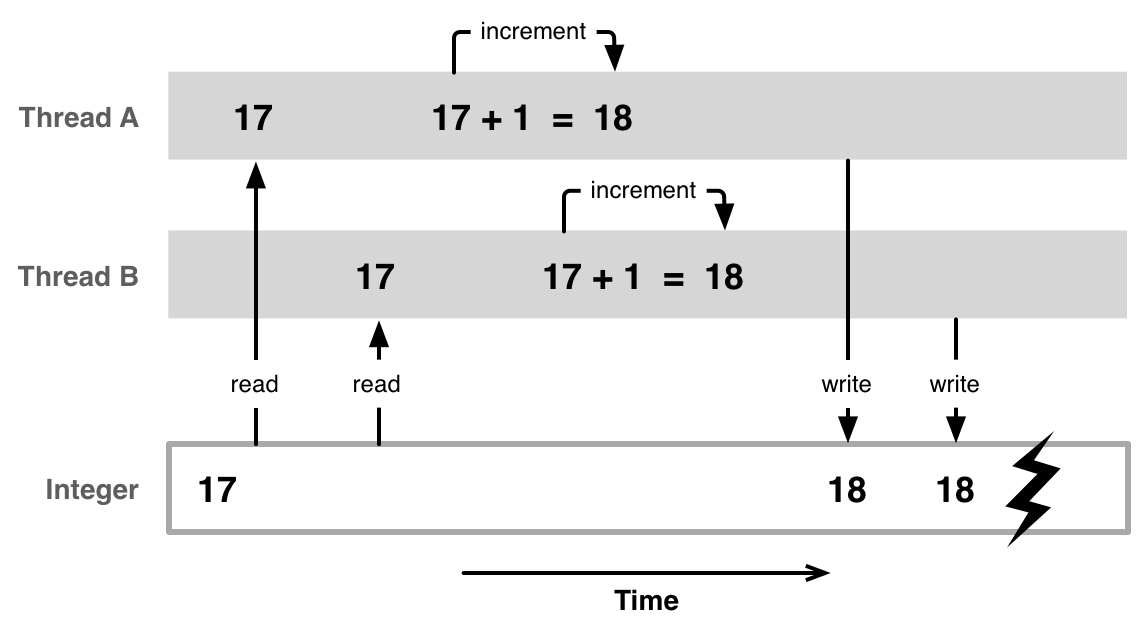
\includegraphics[width=115mm]{images/race-condition.png}
    \cite{Race-Condition}
    \label{fig:race-condition}
\end{figure}

\subsection{Mutual Exclusion}\label{subsec:mutual-exclusion}

As discussed, mutual exclusion does only allow one process or thread to access the shared resource at a time. This includes that if a process p1 already accessed the shared resource x and is still working on it, a second process p2, which tries to access that shared resource x has to wait until the process p1 finishes its task, where it needs that shared resource x. To achieve this, synchronisation techniques based on locks or semaphores are typically used to block the entry of a process to an already accessed and in use shared resource of another process. See \cref{fig:mutual-exclusion} to gain a deeper understanding on how this works. This paper will not go into detail how traditional synchronisation techniques like locks or semaphores work, since for this work it is only important that these kinds of methods manage the access of processes to shared resources in shared memory via some kind of locks. A process will acquire a lock to access a shared resource and will release it when its task is done. Another process trying to access the same resource while it's in use has to wait until the lock is released for that resource.

\begin{figure}[!ht]
    \centering
    \captionsetup{justification=centering}
    \caption{Mutual exclusion between three tasks(processes), which access the same critical section. Multiple processes need to stop working and just wait for other processes to finish their work. See the waiting phase of the processes.}
    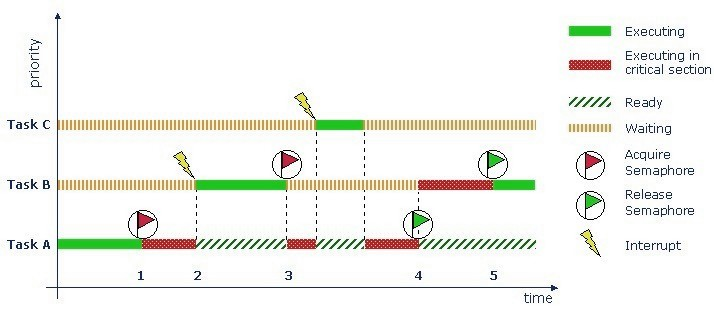
\includegraphics[width=135mm]{images/mutual_exclusion.jpg}
    \cite{MutualExclusion}
    \label{fig:mutual-exclusion}
\end{figure}

Clearly, this approach inherently relies on blocking processes. This may lead to several issues, including deadlocks, process starvation, or priority inversion leading to unpredictable response times not being able to define timing constraints for \ac{RTS} \cite{brandenburg2019multiprocessorrealtimelockingprotocols}. The sequence which process might acquire the lock first to enter the critical section, when multiple processes wait for the access is mostly set by a scheduler \cite{brandenburg2019multiprocessorrealtimelockingprotocols}. Since wait-free methods explained later in \cref{sec:wait-free} are lock-free, a scheduler is not needed and as a result of that scheduling will not be explained more in detail in this work. The problems mentioned above will be discussed in the following subsubsections:

\begin{figure}[!ht]
    \centering
    \captionsetup{justification=centering}
    \caption{Deadlock between two processes, which wait for each other to release the needed resources.}
    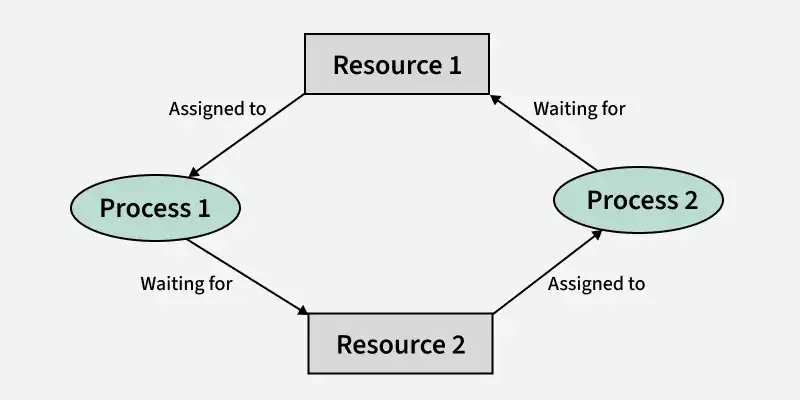
\includegraphics[width=110mm]{images/deadlock.png}
    \cite{Deadlock}
    \label{fig:deadlock}
\end{figure}

\subsubsection{Process Starvation}\label{subsubsec:process-starvation}

What happens when multiple processes try to enter the shared resource one after another, and one process repeatedly fails to acquire a lock to enter the critical section. This one  process would wait for an indefinite time and will never enter the shared resource, which is called as process starvation. This usually happens when a synchronisation method allows one or more processes to make progress while ignoring a particular process or processes. This mostly happens in environments where some sort of process prioritisation exists and processes are classified into low and high priority processes. When there are always a lot of high priority and some low priority processes available, it might happen that these low priority processes will never be able to enter the critical section. This is a problem, since these low priority processes might be important for the system too. \cite{Starvation}

\subsubsection{Deadlock}\label{subsubsec:deadlock}

Even worse, what if two or more processes have already accessed a resource and now each waits for the other to release the lock for the resource each of them acquired to furtther work? This results in a situation seen in \cref{fig:deadlock} where these processes now indefinitely wait for each other and never terminate. Thus, the resources held by these waiting processes are never released and are therefore never available to the other process. As one can see, this brings a system into a state which would make no progress any further and would not respond to any command anymore. \cite{chahar2013deadlock}

For instance, a driverless car with a brake-by-wire system, where processes responsible for braking are in a deadlock, the car could eventually not brake if needed and a fatal collision would happen. 


\subsubsection{Priority Inversion}\label{subsubsec:priority-inversion}

Now let's say no process starvations or deadlocks happen. What could happen too is that a lower priority process already accessed a shared resource and after that a higher priority process needs to access that specific resource too. If the lower priority process now gets delayed, the higher priority process gets delayed too. This would be called priority inversion now; a low priority process delaying a high priority process. \cite{priorityInversion}

\section{Lock-Free Synchronisation}\label{sec:lock-free}

Because of all the problems traditional synchronisation techniques introduce, synchronisation techniques are required that do not block processes with any kind of locking mechanism. One way could be the implementation of lock-free synchronisation techniques. This would allow multiple processes to access the shared resource concurrently. Lock-free synchronisation ensures that at least one process will complete its task in a finite number of steps. However, some processes may be unable to proceed, because lock-free synchronisation does not guarantee that all processes will complete their operations in a finite number of steps. This means that starvation or even priority inversion is still possible, as some processes, even high priority processes may be indefinitely delayed. There are different kinds of mechanisms to achieve this. One way to accomplish lock-freedom for example is the lock-free technique introduced by Michael and Scott, which is also the basis for some other wait-free algorithms.

\subsection{Michael and Scott's Lock-Free Queue}\label{subsec:michael-scott}

Michael and Scott developed an algorithm seen in \cref{alg:michael-scott} using a linked-list as a shared data structure with an enqueue and a dequeue function to introduce lock-freedom. A linked-list is a list containing nodes containing data and a pointer called next which references the next node in the list, which can only be traversed in a single direction. There is also a pointer called head, which references the beginning node of the list and a pointer called tail, which references the end node of the list. The core concept of the algorithm is the enqueue and dequeue functions beginning at lines 7 and 26 in \cref{alg:michael-scott}, which are used to add and remove nodes to the shared data structure. When a process tries to add a node to the list, it first creates a new node and sets its next pointer to \texttt{NULL}, see line 8 to 10 of the enqueue function. Beginning from line 11 to line 23 following happens: The process first checks if the pointer referencing to the next node after the tail node is \texttt{NULL}, see line 15. If it is \texttt{NULL} it tries to link the new node to the end of the list by using a \ac{CAS} seen in line 16. This operation atomically compares the current value of the tail pointer with the expected value and, if they match, updates the tail pointer to point to the new node. The tail itself would be updated in line 24.  \cite{MichaelScottQueue}

So let's say 2 processes p1 and p2 execute up to line 16 one after the other. What could happen now is that if p1 executes line 16 before p2, p2 will fail the \ac{CAS} from line 16. Now if p1 does not execute further, thus not finalising the enqueue with line 24 and p2 retries the loop until line 15, the condition in line 15 would not be \texttt{TRUE} anymore for p1 and p1 would execute lines 19 and 20 to help p2 to finalise its enqueue so other processes can work further with this algorithm. \cite{MichaelScottQueue}

The dequeue function works analogously, but instead of adding a node to the end of the list it removes a node from the front of the list. And since another process which could not finish its enqueue would cause confusion for other processes in the dequeue function, the process which could not finish its enqueue will also be helped in the dequeue function. \cite{MichaelScottQueue}

Initialisation starts at line 1 in \cref{alg:michael-scott}, which is just used to create dummy nodes when there's no node in the list. This just simplifies the algorithm so that the head and tail pointers are not \texttt{NULL}. It can be observed that this approach does not need any locks explained in \cref{sec:synchronization}. However, this approach has one major problem. If for instance process p1 is trying to enqueue, it can happen that the \ac{CAS} loop might fail indefinitely if for an indefinite time other processes are always executing line 16 immediately before p1 could execute line 16. This means that in very high contention scenarios, a process may be delayed indefinitely and starve out. In an \ac{HRTS}, this could lead to violation of timing constraints, since the process would not finish his task in the defined timing window, which is unacceptable. This is why a slightly different approach which guarantees that every process will complete its operation in a finite number of steps is in need. \cite{MichaelScottQueue}

\begin{algorithm}[!ht]
    \centering
    \captionsetup{justification=centering}
    \caption{Michael and Scott's Lock-Free Queue}
    \label{alg:michael-scott}
    \scriptsize
    \begin{algorithmic}[1]

    \Function{Initialize}{Q : pointer to queue\_t}
        \State node = \textbf{new} node() 
        \Comment{Allocate a dummy node}
        \State node.next.ptr = \texttt{NULL}
        \Comment{Make it the only node in the list}
        \State Q.Head = node 
        \Comment{Both Head and Tail point}
        \State Q.Tail = node 
        \Comment{to this dummy node}
    \EndFunction
    
    \Function{Enqueue}{Q : pointer to queue\_t, value : data\_type}
        \State node = \textbf{new} node() 
        \Comment{Allocate a new node from the free list}
        \State node.value = value
        \Comment{Copy enqueue value into node}
        \State node.next.ptr = \texttt{NULL}
        \Comment{Set next pointer of node to NULL}
    
        \Loop 
        \Comment{Keep trying until Enqueue is done}
            \State tail = Q.Tail
            \Comment{Read Tail (pointer + count) together}
            \State next = tail.ptr.next
            \Comment{Read next ptr + count together}
    
            \If{tail == Q.Tail} 
            \Comment{Are tail \& next consistent?}
                \If{next.ptr == \texttt{NULL}}
                \Comment{Tail is the last node?}
                    \If{$CAS(\&\,tail.ptr.next,\; next,\; \langle node,\; next.count+1\rangle)$}
                        \State \textbf{break}
                        \Comment{Link the new node; Enqueue is done}
                    \EndIf
                \Else 
                \Comment{Tail not pointing to the last node}
                    \State CAS($\&$\,Q.Tail,\; tail,\; $\langle$ next.ptr,\; tail.count+1$\rangle$)
                    \Comment{Move Tail forward (helping another enqueuer)}
                \EndIf
            \EndIf
        \EndLoop
    
        \State 
        $CAS(\&\,Q.Tail,\; tail,\; \langle node,\; tail.count+1\rangle)$
        \Comment{Final attempt to swing Tail to the inserted node}
    
    \EndFunction
    
    \Function{Dequeue}{Q : pointer to queue\_t,\; pvalue : pointer to data\_type}
        \Loop
        \Comment{Keep trying until Dequeue is done}
            \State head = Q.Head
            \State tail = Q.Tail
            \State next = head.ptr.next
            \Comment{Read head->next}
    
            \If{head == Q.Head} 
            \Comment{Still consistent?}
                \If{head.ptr == tail.ptr} 
                \Comment{Empty or Tail behind?}
                    \If{next.ptr == \texttt{NULL}}
                    \Comment{Queue is empty}
                        \State \textbf{return} FALSE
                    \Else
                        \Comment{Tail is behind, help move it}
                        \State 
                        $CAS(\&\,Q.Tail,\; tail,\; \langle next.ptr,\; tail.count+1\rangle$)
                    \EndIf
    
                \Else
                    \Comment{No need to adjust Tail}
                    \State *pvalue = next.ptr.value
                    \Comment{Read value before CAS}
                    \If{$CAS(\&\,Q.Head,\; head,\; \langle next.ptr,\; head.count+1\rangle)$}
                        \State \textbf{break}
                        \Comment{Dequeue is done}
                    \EndIf
                \EndIf
            \EndIf
        \EndLoop
    
        \State \textbf{free}(head.ptr)
        \Comment{Safe to free old dummy node}
        \State \textbf{return} TRUE
    
    \EndFunction
    
    \end{algorithmic}
    \cite{MichaelScottQueue}
\end{algorithm} 

While Michael and Scott's algorithm relies on the \ac{CAS} primitive, other atomic primitives provide alternative approaches that other algorithms shown later in this thesis use. An overview on the atomic primitives that are used in this thesis context is given in the following section.

\subsection{Atomic Primitives}\label{subsec:atomic-primitives}
Atomic primitives are hardware instructions that conduct a set of steps atomically, meaning with no interruption from other processes \cite{Atomics}. This will be important in the algorithms analysed later in this thesis, since these primitives are used to implement wait-free synchronisation. There are different kinds of atomic primitives: 

\subsubsection{\acf{LL/SC}}\label{subsubsec:llsc}
Abbreviation of the instructions \ac{LL} and \ac{SC}, which is an operation available on ARM, MIPS and Alpha architectures usually implied with a \ac{VL} instruction.
\begin{itemize}
    \item \ac{LL}(R) returns value of register r
    \item \enquote{\ac{SC}(R, v) changes the value in register R to v and returns true, if and only if no other process performed a successful SC since the most recent call of LL of the current process. So SC fails if the value of the register has changed since it has been read} \cite{Fuchs2014EvaluationOT}
    \item \enquote{\ac{VL}(R) returns true if no other process performed a successful SC on register R, which allows to test a register value without changing it} \cite{Fuchs2014EvaluationOT}
\end{itemize}
\cite{Fuchs2014EvaluationOT}

\subsubsection{\acf{CAS}}\label{subsubsec:compare-and-swap}
In addition to the explanation in \cref{subsec:michael-scott} \ac{CAS} is an atomic primitive that is supported on \enquote{Intel x386, x64 and most general purpose architectures with operands that are restricted to pointer size} \cite{Fuchs2014EvaluationOT}.
\begin{itemize}
    \item \enquote{\ac{CAS}(R,e,n) returns true and sets the value of R to n if the value in R is e. Otherwise, it returns false.} \cite{Fuchs2014EvaluationOT}
\end{itemize}
The problem with \ac{CAS}, beyond the issue explained earlier, in \cref{subsec:michael-scott} is that it can lead to the ABA problem, which can also occur in wait-free algorithms:
\begin{itemize}
    \item Process 1 reads value A from a shared variable.
    \item Process 2 changes the value to B and then back to A.
    \item Process 1's \ac{CAS} operation succeeds, because it compares the value A it read earlier with the current value A, even though the value was changed in between.
\end{itemize}
This is a fundamental limitation of \ac{CAS}. One solution would be to replace \ac{CAS} with \ac{LL/SC}, but that is not possible on x86 processors. So other solutions are needed that are discussed in \cref{ch:implementation}. \cite{Fuchs2014EvaluationOT}

\subsubsection{\ac{DWCAS}}\label{subsubsec:double-compare-and-swap}
This is a \ac{CAS} on two neighbouring memory locations. \cite{Fuchs2014EvaluationOT}

\subsubsection{\ac{DCAS}}\label{subsubsec:double-with-compare-and-swap}
Sometimes also called \ac{CAS}2, is a \ac{CAS} on two independent memory locations. \cite{Fuchs2014EvaluationOT}

\subsubsection{Swap}\label{subsubsec:swap}
Swap is an atomic read-modify-write operation that unconditionally exchanges a value in memory with a new value and returns the old value. Swap(R, v) atomically stores value v into location R and returns the previous value that was in R. This operation always succeeds. \cite{Mateíspmc}.

\subsubsection{\acf{FAA}}\label{subsubsec:fetch-and-add}
This primitive is used to increment \enquote{the value of a variable by a given offset and [return] the result. This instruction always succeeds.} \cite{Fuchs2014EvaluationOT}

\subsubsection{\ac{FAS}}\label{subsubsec:fetch-and-store}
This atomically stores a value in a variable and returns the previous value. This is similar to \ac{CAS}, but it does not require a comparison and a retry loop. This is faster than \ac{CAS}, if conditions before updating do not need to be checked. \cite{Drescher2015GuardedSections}

\section{Wait-Free Synchronisation}\label{sec:wait-free}

Lock-freedom solves the problem of a system getting into a deadlock. But this is not enough, in a fully automated car for example it is undesirable that any process does not complete its task, since that could mean that some processes that are responsible for braking would not finish their work in a worst case scenario. And such an occasion where the car would need to brake a fatal collision would be the outcome. Consequently, a solution is necessary where every process finishes their task in a finite number of steps instead of just one process. So something is needed that builds upon such mechanisms and extends them. This is exactly what wait-free synchronisation is. It guarantees that every process will complete its operation in a finite number of steps, regardless of contention. This means that even process starvation is by definition not possible anymore. Also priority inversion is eliminated too, because processes do not have to wait for other processes anymore. This ensures system responsiveness and predictability therefore the ability to define strict timing constraints needed for \ac{HRTS} applications. But even wait-free algorithms introduce one problem. Wait-free algorithms are in most cases slower than their lock-free counterparts in execution. A solution for this will be addressed in \cref{ch:related-work} and analysed more in depth in \cref{ch:choosing-the-optimal-wait-free-data-structure}.

\section{Rust Programming Language}\label{sec:rust}

The question now is which programming language suits best for this kind of algorithms. Since a fast communication between the processes is compulsory to meet all \ac{HRTS} timing constraints, the C programming language would be a good choice. C provides low-hardware control and therefore also allows the implementation of fast low-latency communication. What is also important and necessary for a \ac{RTS} is that C does not have an automatic garbage collector, which gets active and stops all processes from working to clean up allocated but no longer used memory space. Because of that all \ac{RTOS} are written in C. The main problem with C is that it does not provide any kind of memory safety, since C implements memory operations that are prone to buffer overflows or control-flow attacks. In the industry around 70\% of vulnerabilities happen due to memory safety issues. If the real-time application would run on an isolated system with no internet connection, this would not be a problem. But in modern automation, where systems need to be connected to the internet for data exchange, such systems would be prone to security attacks. \ac{RTS} nowadays is an integral part in various connected devices, including critical fields such as health or transportation. Consequently, it is extremely important that the security of such devices is guaranteed. With the Rust programming language the problems of memory safety are gone. The difference to C is that it can be as fast as C with the possibility to support low-level control and high-level programming features, while providing memory safety features. The memory safety aspect is achieved by an ownership concept that controls how memory is handled in programmes. This is strictly checked and therefore the executable programme has guaranteed memory safety. In the model every value has a single owner represented by a variable. The owner is in charge of the lifetime and deallocation of that value. Rust will automatically free the memory associated with that value, when the owner goes out of scope. This behaviour is automatically done by using the memory reference feature provided by Rust. Creating such references is called borrowing. This allows the usage of these values without transferring the ownership. These references have their own lifetime, which can be explicitly defined by the programmer or implicitly inferred by Rust's compiler. This ensures that the references are valid and do not exist longer than needed. Hence this can play a role in lock-freedom, which is needed for wait-free synchronisation, since shared resources can be shared with this ownership concept. Additionally, Rust is a type-safe language, which can be helpful during implementation to avoid bugs and errors. As seen, Rust is a good choice for implementing wait-free synchronisation mechanisms for \ac{IPC} in \ac{RTS}. \cite{xu2023rust, culic2022lowRust}. 

Further mechanisms on how Rust handles different kinds of common memory safety issues are solved will not be discussed in detail, as that would go beyond the scope of this thesis. It is only important to know the basics on how Rust is a type-safe and memory-safe programming language, to understand why Rust is used for this work.

    \chapter{Related Work}
    \chapter{Methodology}
    \chapter{Choosing the Optimal Wait-Free Data Structure and algorithm}\label{ch:choosing-the-optimal-wait-free-data-structure}

\section{Optimal Wait-Free Data Structure}\label{sec:optimal-wait-free-data-structure}

An important question is what data structure to use for the implementation of a wait-free synchronisation technique for \ac{IPC}. M. Herlihy showed that every data structure can be made wait-free \cite{herlihy1991wait}. So it is important to choose the optimal data structure for our use. Considering that the reason of this work is to optimize modern manufacturing and automation, some form of correct data flow order is as well necessary for correct work flow for instance in an modern manufacturing line or more critical in a driverless car. From that point on we can think of an already natural fit like \ac{FIFO} queues. Natural because in such queues a producer process can enqueue messages and the consumer process can dequeue messages sequentially. This models real-world data flows (sensor readings, commands, network packets), which are inherently sequential. Consequently with such queues the order of the data flow is preversed without the need of implementing additional functionalities. In contrast, data structures like stacks, sets, or maps do not maintain this kind of arrival order and moreover add semantics like \ac{LIFO} order or key-value pairs, which are in most cases not desired or even unnecessary. This would bring in the need of additional functions to just get rid of undesired side effects. Furthermore in a queue we only have two operations, an enqueue and an dequeue operation. All the other data structures introduce more operations and therefore more complexity. The less operations we have, the less complex the implementation will be. Because of these advantages and also because of the fact that in most publications in the wait-free domain queues are beeing used, limiting this thesis to queues only is plausible. \cite{jiffy}

\section{Wait-Free Algorithms}\label{sec:wait-free-alg}
As we know now on which data structure we should focus an important question is which algorithms to use. There are different cases where different kind of algorithms make more sense. We will decide this contention dependant. There exist algorithms for \ac{SPSC}, \ac{MPSC}, \ac{SPMC} and \ac{MPMC} queues. Since all of them have different complexity in runtime and space, it is important to choose the right one for the right use case to save resources and have faster execution times to meet the timing constraints of \ac{HRTS}. In modern manufacturing and automation devices are used which can run multiple applications on the single device. This could mean that every application running on that device could be a producer and a consumer to each other and also maybe some single application of all applications running on that device produces data for just a single other consuming application. And maybe some single application is a producer for multiple consuming applications and multiple applications are producers of a single consuming application. So it can be that all cases can occur in just one design. This means that we have to consider all the different cases of contention. In the following sections we will discuss the different cases and their algorithms. We will also implement them and test them performance wise before we will implement a final solution which uses all the algorithms automatically for the right use of contention between applications. And even if only one pattern occurs for different devices it makes sense to implement all of them, so that in an automated system with multiple device only one implementated solution is needed to be installed.

\subsection{Single Producer and Single Consumer}\label{sec:single-producer-and-single-consumer}
This is the most simple form of \ac{IPC}. In \ac{SPSC} there is no contention from other processes, because we only have one producer and one consumer. The producer can enqueue processes without any other process interfering. The same goes for the consumer. Here only lockfreedom between writer and reader process is sufficient to achieve wait-freedom.

\subsection{Multiple Producer and Single Consumer}\label{sec:multiple-producer-and-single-consumer}

\subsection{Single Producer and Multiple Consumer}\label{sec:single-producer-and-multiple-consumer}

\subsection{Multiple Producer and Multiple Consumer}\label{sec:multiple-producer-and-multiple-consumer}
    \chapter{Implementation}\label{ch:implementation}

After the wait-free algorithms got identified and analyzed the next sub-goal to find the best wait-free algorithms is to implement them like already said in \cref{sec:objective}. The algorithms got implemented and published in the accompanying GitHub repository in \cite{githubMA}, where complete implementation of the algorithms can be found. This chapter will present the implementation details of the concurrent queue algorithms seen in \cref{ch:choosing-the-optimal-wait-free-data-structure} in Rust, focusing on the adaptations necessary for \ac{IPC} over shared memory. While the algorithmic logic of each queue has been discussed already in \cref{ch:choosing-the-optimal-wait-free-data-structure}, the implementation required slight deviations to support \ac{IPC} over shared memory. This includes ensuring correct cache allignment, correctly implementing various atomic primitives, and correctly implementing the logic for shared memory support based on short example snippets of the actual rust implementation from the GitHub repository or some general examples. This does not include showing again the same algorithmic logic just in a actual programming language instead of pseudocode, since that would be redundant. This chapter will give the necessary details to understand how to implement the algorithms in Rust and how to adapt them for \ac{IPC} over shared memory.

\section{Shared Memory Management for Inter-Process Communication}

\ac{IPC} through shared memory requires slightly different approaches compared to multi-threaded heap-based communication. The primary constraint is that shared memory regions may be mapped at different virtual addresses in different processes, requiring all data structures to be completely position-independent. Additionally, dynamic memory allocation is not possible within shared memory regions, necessitating buffer allocation from a pre-allocated memory pool for all dynamic data structures. Threads on the other hand can use the process-private heap for dynamic memory allocation, which' memory layout is shared between threads on the same process, but not processes.  

\subsection{Shared Memory Size Calculation}

Each queue provides a method to calculate the exact shared memory size required. This calculation determines how much memory to allocate from the operating system. The following examples from BQueue and \ac{wCQ} demonstrate both simple and complex size calculations as needed:

\begin{lstlisting}[language=Rust, style=boxed, caption={Shared memory size calculation methods}, label={lst:size-calculation}]
// From BQueue - simple calculation
pub const fn shared_size(capacity: usize) -> usize {
    mem::size_of::<Self>()                              // Queue structure
        + capacity * mem::size_of::<MaybeUninit<T>>()   // Data storage
        + capacity * mem::size_of::<AtomicBool>()       // Validity flags
}

// From WCQueue - complex layout calculation
fn layout(num_threads: usize, num_indices: usize) -> (Layout, [usize; 4]) {
    let ring_size = num_indices.next_power_of_two();
    let capacity = ring_size * 2;
    
    let root = Layout::new::<Self>();
    let (l_aq_entries, o_aq_entries) = root
        .extend(Layout::array::<EntryPair>(capacity).unwrap())
        .unwrap();
    let (l_fq_entries, o_fq_entries) = l_aq_entries
        .extend(Layout::array::<EntryPair>(capacity).unwrap())
        .unwrap();
    let (l_records, o_records) = l_fq_entries
        .extend(Layout::array::<ThreadRecord>(num_threads).unwrap())
        .unwrap();
    let (l_final, o_data) = l_records
        .extend(Layout::array::<DataEntry<T>>(num_indices).unwrap())
        .unwrap();
    
    (l_final.pad_to_align(), [o_aq_entries, o_fq_entries, o_records, o_data])
}

pub fn shared_size(num_threads: usize) -> usize {
    let (_layout, _offsets) = Self::layout(num_threads, num_indices);
    _layout.size()  // Total bytes needed for mmap
}
\end{lstlisting}

The size calculation accounts for all components including alignment padding. Some queues like \ac{wCQ} use Rust's \texttt{Layout} API shown in lines 9 to 26 to ensure proper alignment and correctly calculated offsets. For simple queues like BQueue, manual calculation like in lines 2 to 6 suffices.

\subsection{Shared Memory Allocation}

Once the required size is calculated, the following functions in \cref{lst:map-shared} used in all benchmarks demonstrates how to allocate and deallocate the needed shared memory regions using \texttt{mmap}:

\begin{lstlisting}[language=Rust, style=boxed, caption={Shared memory allocation using mmap}, label={lst:map-shared}]
unsafe fn map_shared(bytes: usize) -> *mut u8 {
    let ptr = libc::mmap(
        ptr::null_mut(),
        bytes,                                    // Size from shared_size()
        libc::PROT_READ | libc::PROT_WRITE,
        libc::MAP_SHARED | libc::MAP_ANONYMOUS,   // Shared between processes
        -1,
        0,
    );
    if ptr == libc::MAP_FAILED {
        panic!("mmap failed: {}", std::io::Error::last_os_error());
    }
    ptr.cast()
}

// Cleanup function
unsafe fn unmap_shared(ptr: *mut u8, len: usize) {
    if libc::munmap(ptr.cast(), len) == -1 {
        panic!("munmap failed: {}", std::io::Error::last_os_error());
    }
}
\end{lstlisting}

The \texttt{MAP\_SHARED} flag ensures that modifications to the memory region are visible to all processes that map it. The \texttt{MAP\_ANONYMOUS} flag creates memory not backed by a file. The \texttt{bytes} parameter on line 4 comes directly from the \texttt{shared\_size()} calculation earlier.

\subsection{Memory Layout and Initialization}

After allocating the shared memory region the components needed by the queue's implementations need to be initialized. All queue implementations follow a consistent pattern for shared memory initialization. The initialization function receives the pre-allocated memory pointer and organizes components within that memory region. The most complex example, the WCQueue from \cref{subsubsec:wcq}, demonstrates how multiple components are laid out in shared memory with proper alignment:

\begin{lstlisting}[language=Rust, style=boxed, caption={Memory layout initialization in WCQueue}, label={lst:wcqueue-init}]
pub unsafe fn init_in_shared(mem: *mut u8, num_threads: usize) -> &'static mut Self {
    let mut current_offset = 0usize;
    
    // Align and place queue structure
    current_offset = (current_offset + self_align - 1) & !(self_align - 1);
    let q_ptr = mem.add(current_offset) as *mut Self;
    current_offset += mem::size_of::<Self>();
    
    // Align and place entry arrays
    current_offset = (current_offset + entry_align - 1) & !(entry_align - 1);
    let aq_entries = mem.add(current_offset) as *mut EntryPair;
    current_offset += capacity * mem::size_of::<EntryPair>();
    
    // Initialize structures in-place
    ptr::write(q_ptr, Self {
        aq_entries_offset: current_offset,
        base_ptr: mem,  // Store base pointer for offset calculations
        // Store offsets instead of pointers
    });
    
    &mut *q_ptr
}
\end{lstlisting}

The alignment calculation in line 5 ensures that each component starts at a properly aligned address. This is crucial for atomic operations, which often require natural alignment. The queue structure stores offsets relative to the base pointer rather than absolute pointers in line 16, ensuring position independence. When accessing these components later, the offset is added to the base pointer, as demonstrated in \cref{lst:position-independent}.

\begin{lstlisting}[language=Rust, style=boxed, caption={Position-independent component access}, label={lst:position-independent}]
unsafe fn get_entry(&self, entries_offset: usize, idx: usize) -> &EntryPair {
    let entries = self.base_ptr.add(entries_offset) as *const EntryPair;
    &*entries.add(idx)
}
\end{lstlisting}

\subsection{Node Allocation from Pre-allocated Memory Pools}

Some queues as seen in \cref{ch:choosing-the-optimal-wait-free-data-structure} use dynamic memory allocation within the process-private heap. For the \ac{IPC} over shared memory use-case of this thesis that is not possible, because in shared memory dynamic memory allocations or deallocations with \texttt{malloc} or \texttt{free} are not possible, since that allocates from process-private heaps that are not available for other processes. Therefore, all queues that would normally allocate memory dynamically have been adapted to allocate from the initialized pre-allocated memory pool. As an example the Jiffy Queue algorithm from \cref{subsubsec:jiffy-mpsc-queue} shows a dynamic heap allocation method to allocate new buffers to insert them into the linked-list. This was adapted to \ac{IPC} over shared memory in rust by a pool allocation system with free lists that is similarly impülemented for all other queues needing dynamic memory allocation, as shown in \cref{lst:pool-allocation}.

\begin{lstlisting}[language=Rust, style=boxed, caption={Lock-free memory pool allocation}, label={lst:pool-allocation}]
unsafe fn alloc_node_array_slice(&self) -> *mut Node<T> {
    // Try reuse from free list first
    loop {
        let free_head = self.node_array_slice_free_list_head.load(Ordering::Acquire);
        if free_head.is_null() {
            break;
        }
        
        let next_free = (*(free_head as *mut AtomicPtr<Node<T>>))
            .load(Ordering::Acquire);
            
        if self.node_array_slice_free_list_head.compare_exchange(
            free_head, 
            next_free, 
            Ordering::AcqRel, 
            Ordering::Acquire
        ).is_ok() {
            return free_head;
        }
    }
    
    // Allocate from pre-allocated pool
    let nodes_needed = self.buffer_capacity_per_array;
    let start_idx = self.node_arrays_next_free_node_idx
        .fetch_add(nodes_needed, Ordering::AcqRel);
        
    if start_idx + nodes_needed > self.node_arrays_pool_total_nodes {
        self.node_arrays_next_free_node_idx
            .fetch_sub(nodes_needed, Ordering::Relaxed);
        return ptr::null_mut(); // Pool exhausted
    }
    
    self.node_arrays_pool_start.add(start_idx)
}
\end{lstlisting}

This implementation maintains a free list using \ac{CAS} operations in lines 12 to 16. When the free list is empty, it falls back to allocate from the pre-allocated pool seen in lines 23 and 24. The \texttt{fetch\_add} operation atomically increments the allocation index, ensuring process-safe allocation. If the pool is exhausted, the operation fails by returning a null pointer in line 30.

\section{Cache Line Optimization}
Processors transfer data between cores in cache line units explained in \cref{subsubsec:lamport-circular-buffer-queue}. When multiple processes access data on the same cache line, even if different variables, the cache coherence protocol causes the cache line to bounce between cores, degrading execution times.

\subsection{Explicit Cache Line Padding}

In \cref{ch:choosing-the-optimal-wait-free-data-structure} multiple queues were shown that describe seperating the cache line. To show how this is done in rust the \ac{BLQ} explained in \cref{subsec:single-producer-and-single-consumer} will be taken to show how to explicitly seperate the cache lines, as shown in \cref{lst:cache-separation}.

\begin{lstlisting}[language=Rust, style=boxed, caption={Cache line separation in BlqQueue}, label={lst:cache-separation}]
const CACHE_LINE_SIZE: usize = 64;

#[repr(C)]
#[cfg_attr(any(target_arch = "x86_64", target_arch = "aarch64"), repr(align(64)))]
pub struct SharedIndices {
    pub write: AtomicUsize,  // Producer's cache line
    pub read: AtomicUsize,   // Consumer's cache line
}

#[repr(C, align(64))]
struct ProducerPrivate {
    read_shadow: usize,      // Local copy to avoid false sharing
    write_priv: usize,       // Producer-only write position
}

#[repr(C, align(64))]
struct ConsumerPrivate {
    write_shadow: usize,     // Local copy to avoid false sharing
    read_priv: usize,        // Consumer-only read position
}
\end{lstlisting}

The \texttt{\#[repr(C)]} attribute ensures C-compatible memory layout, while \newline \texttt{\#[repr(align(64))]} forces the structure to start at a cache line boundary shown in lines 4 and 10. Although \texttt{SharedIndices} contains only two \texttt{usize} values with 16 bytes total, the alignment ensures they reside in separate cache lines. The producer updates \texttt{write} while the consumer updates \texttt{read}, preventing false sharing. The shadow copies \texttt{read\_shadow} in line 12 and \texttt{write\_shadow} in line 18 ensures that producer and consumer work on different cache lines, preventing the cache lines to bounce between the producer process and consumer process.

Similarly all queues that need this kind of cache line separation use this pattern to ensure that the producer and consumer do not share cache lines, preventing false sharing leading to cache lines bouncing between cores.

\subsection{Manual Padding Arrays}

For structures where alignment alone is insufficient, manual padding arrays provide a solution, as demonstrated in \cref{lst:manual-padding}. This is used in all queues needing manual padding. As an example the implementation of the David queue explained in \cref{subsubsec:david-queue} uses manual padding.

\begin{lstlisting}[language=Rust, style=boxed, caption={Manual padding for exact cache line control}, label={lst:manual-padding}]
#[repr(C, align(64))]
struct FetchIncrement {
    value: AtomicUsize,
    _padding: [u8; CACHE_LINE_SIZE - std::mem::size_of::<AtomicUsize>()],
}

#[repr(C, align(64))]
struct Node<T> {
    val: Option<T>,
    next: AtomicPtr<Node<T>>,
    _padding: [u8; CACHE_LINE_SIZE - 24], // Fill remaining cache line
}
\end{lstlisting}

The padding array size is calculated to fill the remainder of the cache line seen in lines 4 and 11. For \texttt{FetchIncrement}, the \texttt{AtomicUsize} occupies 8 bytes, so 56 bytes of padding complete the 64-byte cache line. This ensures each \texttt{FetchIncrement} instance occupies exactly one cache line, preventing false sharing in arrays of such structures, as required by the DavidQueue implementation from \cref{subsubsec:david-queue}.

\section{Atomic Primitives Implementation}

The algorithms in \cref{ch:choosing-the-optimal-wait-free-data-structure} all use different kind of atomic primitives. To implement them rust provides a set of atomic operations with explicit memory ordering semantics, allowing control over synchronization order. This section shows how in general the atomic operations from \cref{ch:choosing-the-optimal-wait-free-data-structure} are implemented in Rust across all queues, explained with specific examples. In rust atomic primitives can only be called on atomic types. Hence variables that are used in atomic operations must be defined as atomic types.

\subsection{\acf{FAA}}

The rust implementations of DQueue, BQueue and \ac{wCQ} explained in \cref{ch:choosing-the-optimal-wait-free-data-structure} are a good example, to understand how to implement \ac{FAA} called \texttt{fetch\_add(v, ordering)} in rust.

\begin{lstlisting}[language=Rust, style=boxed, caption={Fetch-and-add with different memory orderings}, label={lst:fetch-and-add}]
// From Jiffy - Allocate multiple nodes at once
let start_node_idx = self
    .node_arrays_next_free_node_idx
    .fetch_add(nodes_needed, Ordering::AcqRel);

// From BQueue - private counter with relaxed ordering
let idx = self.next_item.fetch_add(1, Ordering::Relaxed);

// From WCQueue - with sequential consistency for wait-free algorithm
let seqid = self.tail.fetch_add(1, Ordering::SeqCst);
\end{lstlisting}

In rust \ac{FAA} is a method call on atomic types as seen in line 4. In \cref{lst:fetch-and-add} the memory ordering parameter added as the second argument after the value to add determines the synchronization order of \ac{FAA}. \texttt{Ordering::Relaxed} in line 6 provides no synchronization, suitable for private counters. \texttt{Ordering::AcqRel} in line 3 ensures acquire semantics for the read and release semantics for the write, establishing happens-before relationships as required by the DQueue algorithm. \texttt{Ordering::SeqCst} in line 9 provides the strongest guarantees, ensuring a total order across all sequentially consistent operations, necessary for the complex \ac{wCQ}. One simple solution would be to always use \texttt{Ordering::SeqCst} for all operations, but that would reduce the execution times of the algorithms in a significant way. Consequently it is important to analyze the algorithms from \cref{ch:choosing-the-optimal-wait-free-data-structure} to understand which memory ordering is needed for which operation.

\subsection{\acf{CAS}}

The implementation of \ac{wCQ} shows how to implement \ac{CAS}, called \newline \texttt{compare\_exchange(old\_value, new\_value, ordering\_on\_success, \newline ordering\_on\_failure)} in rust, as shown in \cref{lst:compare-and-swap}.

\begin{lstlisting}[language=Rust, style=boxed, caption={Compare-and-swap variants and usage patterns}, label={lst:compare-and-swap}]
// Strong CAS with sequential consistency (from wcqueue)
match entry.value.compare_exchange(
    packed,
    new_packed,
    Ordering::SeqCst,    // Success ordering
    Ordering::SeqCst,    // Failure ordering
) {
    Ok(_) => {
        fence(Ordering::SeqCst);  // Additional synchronization
        Ok(())
    }
    Err(current) => {
        // Retry with current value
    }
}

// Weak CAS for performance (general example)
match entry.value.compare_exchange_weak(
    old_value,
    new_value,
    Ordering::AcqRel,
    Ordering::Acquire,
) {
    Ok(_) => {
        // do something on success
    }
    Err(current) => {
        // do something on failure
    }
}
\end{lstlisting}

The weak variant \texttt{compare\_exchange\_weak} in beginning at 17 may fail spuriously even when the values match, but can be more efficient on some architectures. The strong variant guarantees success when values match. The two ordering parameters in line 5 and 6 and 21 and 22 specify synchronization order for success and failure cases respectively at lines 8 and 12. This directly implements the CAS operations described in multiple algorithms.

\subsection{Swap Operations}

Swap unconditionally replaces a value and returns the previous value, implemented as \texttt{swap(new\_value, ordering)}, as shown in \cref{lst:swap-operations}. As an example the David Queue and Drescher Queue is used.

\begin{lstlisting}[language=Rust, style=boxed, caption={Unconditional atomic swap operations}, label={lst:swap-operations}]
// From David Queue - unconditional slot update
unsafe fn swap(&self, new_val: usize) -> usize {
    self.value.swap(new_val, Ordering::AcqRel)
}

// From Drescher Queue - atomic pointer swap
let prev_tail = self.tail.swap(new_node_ptr, Ordering::AcqRel);

// From DrescherQueue - simpler FAS primitive
let prev_tail_ptr = self.tail.swap(new_node_ptr, Ordering::AcqRel);
(*prev_tail_ptr).next.store(new_node_ptr, Ordering::Release);
\end{lstlisting}

Swap operations are useful when the previous value is needed but the update is unconditional. The DrescherQueue uses swap to implement its simple enqueue operation (line 10), atomically updating the tail pointer and then linking the previous tail to the new node, exactly as specified in the Drescher algorithm in \cref{subsubsec:drescher-mpsc-queue}.

\subsection{Load and Store with Memory Ordering}

Simple loads and stores also require consideration of memory ordering to ensure correct synchronization according to the algorithms in \cref{ch:choosing-the-optimal-wait-free-data-structure}, as demonstrated in the general example of \cref{lst:load-store}.

\begin{lstlisting}[language=Rust, style=boxed, caption={Memory ordering for loads and stores}, label={lst:load-store}]
// Acquire ordering for reading shared state
let tail = self.tail.load(Ordering::Acquire);
if tail > head {
    // Safe to proceed - acquire ensures we see all writes before tail update
}

// Release ordering for publishing updates
unsafe { (*slot.data.get()).write(item); }  // Write data first
self.head.store(new_head, Ordering::Release);  // Then publish

// Sequential consistency for strong synchronization
let val = entry.value.load(Ordering::SeqCst);
entry.value.store(new_val, Ordering::SeqCst);
\end{lstlisting}

The acquire-release pattern is particularly important. A release store in line 9 synchronizes with an acquire load in line 2 of the same location, ensuring that all writes before the release store are visible to any thread that sees the acquire load. This pattern is used in all queues to ensure correct ordering to the producer-consumer relationship, implementing the memory barriers described in algorithms like Lamport Queue (\cref{subsubsec:lamport-circular-buffer-queue}) and others.

\subsection{Memory Fences}

To still ensure correct data ordering without any memory operation rust provide memeory fencec seen in the \ac{wCQ} rust implementation, as shown in \cref{lst:memory-fences}.

\begin{lstlisting}[language=Rust, style=boxed, caption={Explicit memory fence usage}, label={lst:memory-fences}]
// From WCQueue - ensuring visibility across operations
fence(Ordering::SeqCst);
let packed = entry.value.load(Ordering::SeqCst);
let e = EntryPair::unpack_entry(packed);

if condition {
    fence(Ordering::SeqCst);  // Ensure all prior operations complete
    
    match entry.value.compare_exchange_weak(
        packed,
        new_packed,
        Ordering::SeqCst,
        Ordering::SeqCst,
    ) {
        Ok(_) => {
            fence(Ordering::SeqCst);  // Ensure visibility before proceeding
        }
    }
}
\end{lstlisting}

Fences ensure ordering between operations that might not otherwise synchronize. The \ac{wCQ} implementation uses sequential consistency fences (lines 2, 7, 16) to ensure correctness in its complex algorithm. These kind of fences are used in all queue implementations since for \ac{IPC} this was necessary for correrctness. 

\subsection{Versioned \acf{CAS} (Simulating \acf{LL/SC})}

Some algorithms assume \ac{LL/SC} primitives, which x86-64 does not provide. The \ac{JPQ} from \cref{subsub:jayanti-mpsc-queue} simulates \ac{LL/SC} using versioned \ac{CAS}, as shown in \cref{lst:versioned-cas}.

\begin{lstlisting}[language=Rust, style=boxed, caption={Versioned CAS for LL/SC simulation}, label={lst:versioned-cas}]
#[repr(C)]
struct CompactMinInfo {
    version: u32,    // Version counter for ABA prevention
    ts_val: u16,     // Timestamp value (compressed)
    ts_pid: u8,      // Process ID (compressed)  
    leaf_idx: u8,    // Leaf index (compressed)
}

impl CompactMinInfo {
    fn to_u64(self) -> u64 {
        ((self.version as u64) << 32)
            | ((self.ts_val as u64) << 16)
            | ((self.ts_pid as u64) << 8)
            | (self.leaf_idx as u64)
    }
}

unsafe fn cas_min_info(&self, old_compact: CompactMinInfo, 
                       new_min_info: MinInfo) -> bool {
    // Increment version on every update
    let new_compact = CompactMinInfo::from_min_info(
        new_min_info, 
        old_compact.version + 1
    );
    
    self.compact_min_info.compare_exchange(
        old_compact.to_u64(),
        new_compact.to_u64(),
        Ordering::AcqRel,
        Ordering::Acquire
    ).is_ok()
}
\end{lstlisting}

The version counter in line 3 prevents the ABA problem where a value changes from A to B and back to A between observations. By incrementing the version on every update seen in line 23, even if the logical value returns to a previous state, the version ensures the \ac{CAS} will fail, simulating \ac{LL/SC} semantics as required by the \ac{JPQ} algorithm. This is done in every queue rust implementation that requires \ac{LL/SC} semantics.

\subsection{Unsafe Blocks}

Rust's memory safety guarantees to prevent data races by ensuring that either multiple readers or a single writer can access data at any time. However, the wait-free algorithms in \cref{ch:choosing-the-optimal-wait-free-data-structure} require to bypass these restrictions. With the use of \texttt{unsafe} blocks the the Rust compiler gets indicated that the blocks memory safety is handled by the implementation itself. The \texttt{try\_enq\_inner} function of \ac{wCQ}'s Rust implementation in \cref{lst:wcq-unsafe} demonstrates why \texttt{unsafe} blocks are necessary.

\begin{lstlisting}[language=Rust, style=boxed, caption={Wait-free synchronization requiring unsafe}, label={lst:wcq-unsafe}]
    // Multiple threads may execute this concurrently
    unsafe fn try_enq_inner(&self, wq: &InnerWCQ, entries_offset: usize,
                           index: usize) -> Result<(), u64> {
        let tail = wq.tail.cnt.fetch_add(1, Ordering::AcqRel);
        let j = Self::cache_remap(tail as usize, wq.capacity);
        
        let entry = self.get_entry(wq, entries_offset, j);
        loop {
            let packed = entry.value.load(Ordering::Acquire);
            let e = EntryPair::unpack_entry(packed);
            
            // Check if slot is available
            if e.cycle < Self::cycle(tail, wq.ring_size) &&
               (e.is_safe || wq.head.cnt.load(Ordering::Acquire) <= tail) &&
               (e.index == IDX_EMPTY || e.index == IDX_BOTTOM) {
                
                // Attempt to claim slot with CAS
                match entry.value.compare_exchange_weak(
                    packed,
                    new_packed,
                    Ordering::SeqCst,
                    Ordering::SeqCst,
                ) {
                    Ok(_) => return Ok(()),
                    Err(_) => continue,  // Retry
                }
            }
        }
    }
    
    // get_entry uses raw pointer arithmetic
    unsafe fn get_entry(&self, _wq: &InnerWCQ, entries_offset: usize, 
                       idx: usize) -> &EntryPair {
        let entries = self.base_ptr.add(entries_offset) as *const EntryPair;
        &*entries.add(idx)  // Dereference raw pointer
    }
\end{lstlisting}

One reason for an \texttt{unsafe} block is raw pointer dereferencing seen in lines 32 to 34. The \texttt{get\_entry} function performs pointer arithmetic on \texttt{base\_ptr} and dereferences the result which is needed for shared memory. The compiler cannot verify that the calculated address is valid or that no data races occur. The Rust compiler also does not allow concurrent access of multiple writer threads or processes. \texttt{try\_enq\_inner} beginning at line 2 is implementated so that multiple processes can simultaneously call it. Each process, atomically increments the tail to get a unique position in line 4, then accesses potentially the same entry due to cache remapping in lines 5 and 7, and finally attempts to modify the entry in line 18. The Rust compiler cannot verify too that this access is safe, so the developer of this implementation has to indicate to the compiler that this is safe by using an \texttt{unsafe} block.

\section{Validation}
Part of the objective is also to ensure the correctness of the implemented algorithms, unit and miri tests were performed. The unit tests validate the basic functionality of each queue, ensuring that operations like enqueue and dequeue work as expected. Miri tests were used to check for undefined behavior in concurrent scenarios, ensuring that the algorithms behave correctly under extreme contention. This section will generally describe how the tests were implemented and what they validate, without going into the details of each test case.

\subsection{Basic Operations}
Every queue implementation was validated for fundamental operations including initialization, push, pop, and state queries (\texttt{is\_empty}, \texttt{is\_full}). For example, the basic operation test pattern was implemented as shown in \cref{lst:basic-test}:

\begin{lstlisting}[language=Rust, style=boxed, caption={Basic operation test pattern}, label={lst:basic-test}]
// Test empty queue state
assert!(queue.is_empty());
assert!(queue.pop().is_err());

// Test single element operations
queue.push(42).unwrap();
assert!(!queue.is_empty());
assert_eq!(queue.pop().unwrap(), 42);
assert!(queue.is_empty());

// Test multiple elements
for i in 0..10 {
    queue.push(i).unwrap();
}
for i in 0..10 {
    assert_eq!(queue.pop().unwrap(), i);
}
\end{lstlisting}

Lines 2 to 3 in \cref{lst:basic-test} test the initial empty state and check that pop operations fail correctly on empty queues. The single element test in lines 6 to 9 tests the state change from empty to non-empty and back, with line 8 testing that the pushed value is correctly retrieved. Lines 12 to 17 test that FIFO ordering is maintained for multiple elements.

\subsection{Capacity and Boundary Tests}
Capacity limits also had to be testet, so it can be ensured, that the capacities work correctly. Special attention was given to queues with buffering mechanisms like \ac{BIFFQ} and MultiPush queue, which required explicit flushing operations.

\begin{lstlisting}[language=Rust, style=boxed, caption={Capacity limit test pattern}, label={lst:capacity-test}]
// Test pushing up to capacity
let mut pushed = 0;
for i in 0..capacity {
    match queue.push(i) {
        Ok(_) => pushed += 1,
        Err(_) => break,
    }
}
assert!(pushed > 0, "Should push at least one item");

// Verify queue rejects items when full
assert!(!queue.available() || queue.push(999).is_err());

// Test space recovery after pop
if pushed > 0 {
    assert!(queue.pop().is_ok());
    assert!(queue.available());
    assert!(queue.push(888).is_ok());
}
\end{lstlisting}

In \cref{lst:capacity-test} lines 3 to 8 test filling the queue to capacity, counting successful pushes. Line 9 tests that at least one item could be pushed. Line 12 tests that a full queue either reports no available space or rejects push attempts. Lines 15 to 19 test that after removing an element, space becomes available for new items.

For queues with buffering mechanisms, additional testing was required:

\begin{lstlisting}[language=Rust, style=boxed, caption={Buffered queue capacity test}, label={lst:buffered-capacity-test}]
// BiffQ attempts to push beyond capacity
for i in 0..BIFFQ_CAPACITY + 100 {
    match queue.push(i) {
        Ok(_) => pushed_total += 1,
        Err(_) => {
            // Flush local buffer to main queue
            let _ = queue.flush_producer_buffer();
            if queue.push(i).is_err() {
                break;  // No space in main queue
            } else {
                pushed_total += 1;
            }
        }
    }
    // Periodic flushing every 32 items
    if i % 32 == 31 {
        let _ = queue.flush_producer_buffer();
    }
}
// Final flush to ensure all buffered items are visible
let _ = queue.flush_producer_buffer();

// Verify capacity behavior based on how full the queue got
if pushed_total >= BIFFQ_CAPACITY - 32 {
    // Nearly full: test pop/push with limited space
    assert!(queue.pop().is_ok());
    // Try to push after making space
    for _ in 0..10 {
        let _ = queue.flush_producer_buffer();
        if queue.push(99999).is_ok() {
            break;
        }
        let _ = queue.pop(); // Make more space
    }
} else {
    // Partially full: verify basic push/pop works
    assert!(queue.pop().is_ok());
    assert!(queue.push(99999).is_ok());
}
\end{lstlisting}

The \ac{BIFFQ} test in \cref{lst:buffered-capacity-test} tests the buffering system. When push fails in line 5, line 7 flushes the local buffer to the main queue. If the retry in line 8 still fails, it means the main queue lacks space. Lines 16 to 18 periodically flushes every 32 items (the buffer size). The test in lines 24 to 39 checks different behaviors based on how full the queue is: lines 24 to 33 test the case where the main queue might not have room for a complete buffer flush, while lines 35 to 39 test basic operations when the queue is only partially full.

\subsection{Memory Alignment Verification}
Since the implementations target shared memory with specific alignment requirements, tests as in \cref{lst:alignment-test} verified proper memory alignment for all queue structures:

\begin{lstlisting}[language=Rust, style=boxed, caption={Memory alignment verification test}, label={lst:alignment-test}]
// Allocate memory with specific alignment
let layout = Layout::from_size_align(size, alignment)
    .expect("Invalid layout");
let ptr = unsafe { alloc_zeroed(layout) };

// Verify pointer alignment
assert_eq!(
    ptr as usize % alignment, 0,
    "Memory not aligned to {} bytes", alignment
);

// Initialize queue with aligned memory
let queue = unsafe { 
    <$queue_type>::init_in_shared(ptr, capacity) 
};

// For YangCrummeyQueue requiring 128-byte alignment
let queue_offset = sync_size;
let queue_offset_aligned = (queue_offset + 127) & !127;
let queue_ptr = unsafe { shm_ptr.add(queue_offset_aligned) };
assert_eq!(
    queue_ptr as usize % 128, 0,
    "Queue not properly aligned to 128 bytes"
);
\end{lstlisting}

Lines 2 to 4 in \cref{lst:alignment-test} create memory with the required alignment and allocate it so that lines 7 to 10 can test that the allocation has the correct alignment using modulo arithmetic. For \ac{YMC}, lines 18 and 19 calculate the aligned offset, where \texttt{(offset + 127) \& !127} rounds up to the next 128-byte boundary. Lines 21 to 24 test that the final queue pointer has the required 128-byte alignment.

Position-independent addressing was verified in \cref{lst:position-independent-test} through shared memory tests:

\begin{lstlisting}[language=Rust, style=boxed, caption={Position-independent addressing test}, label={lst:position-independent-test}]
// Map shared memory at arbitrary address
let shm_ptr = unsafe { 
    libc::mmap(
        std::ptr::null_mut(),  // Let OS choose address
        size,
        libc::PROT_READ | libc::PROT_WRITE,
        libc::MAP_SHARED | libc::MAP_ANONYMOUS,
        -1,
        0,
    ) as *mut u8
};

// Initialize queue - must work at any address
let queue = unsafe { 
    Queue::init_in_shared(shm_ptr, capacity) 
};

// Verify queue operates correctly regardless of base address
queue.push(42).unwrap();
assert_eq!(queue.pop().unwrap(), 42);
\end{lstlisting}

Line 4 in \cref{lst:position-independent-test} passes null to let the OS choose the memory address and lines 6 and 7 specify shared anonymous memory for inter-process access. Lines 14 and 15 initializes the at any address. Lines 19 and 20 test that the queue works correctly regardless of its memory location.

\subsubsection{Memory Pool Management}
The pre-allocated memory pools of the queues were tested for correct allocation, recycling, and pool exhaustion handling:

\begin{lstlisting}[language=Rust, style=boxed, caption={Memory pool management test}, label={lst:pool-management-test}]
// Test pool allocation and recycling
unsafe {
    // Allocate from pool
    let seg1: *mut Segment<i32> = queue.new_segment(1);
    assert!(!seg1.is_null());
    assert_eq!((*seg1).id, 1);
    
    // Return to pool
    queue.release_segment_to_pool(seg1);
    
    // Test pool exhaustion
    let mut segments = vec![];
    for i in 2..segment_pool_capacity as u64 {
        let seg = queue.new_segment(i);
        if !seg.is_null() {
            segments.push(seg);
        } else {
            break;  // Pool exhausted
        }
    }
    
    // Return all to pool
    for seg in segments {
        queue.release_segment_to_pool(seg);
    }
}

// Test free list reuse in Jiffy Queue
let free_head = self.node_array_slice_free_list_head
    .load(Ordering::Acquire);
if !free_head.is_null() {
    // Reuse from free list
    let next_free = (*(free_head as *mut AtomicPtr<Node<T>>))
        .load(Ordering::Acquire);
        
    if self.node_array_slice_free_list_head.compare_exchange(
        free_head, 
        next_free, 
        Ordering::AcqRel, 
        Ordering::Acquire
    ).is_ok() {
        return free_head;  // Successfully reused
    }
}
\end{lstlisting}

Lines 4 to 6 in \cref{lst:pool-management-test} test basic allocation from the pool and test that the segment is properly initialized. Line 9 tests returning the segment to the pool. Lines 12 to 20 test pool exhaustion by allocating until \texttt{new\_segment} returns null in line 18. Lines 23 to 25 test that segments can be returned to the pool. Lines 29 to 44 test the free list implementation in Jiffy Queue, where lines 36 to 41 test atomic removal of the free list head using compare-exchange. Since we only test, that the allocations work and can be used, assertions were not used, since only correct behavior is testet.

\subsection{Concurrent Operation Tests}
Concurrent tests validated the correctness of queue operations under contention. Different kinds of tests were implemented to stress the queues in various ways:

\subsubsection{Producer-Consumer Patterns}
Tests spawned separate threads for producers and consumers to test correct concurrent operation as seen in \cref{lst:concurrent-test}:

\begin{lstlisting}[language=Rust, style=boxed, caption={Concurrent test pattern}, label={lst:concurrent-test}]
let barrier = Arc::new(Barrier::new(num_threads));
let mut handles = vec![];

// Spawn producer threads
for tid in 0..num_producers {
    let barrier_clone = barrier.clone();
    let handle = thread::spawn(move || {
        barrier_clone.wait(); // Synchronize start
        for i in 0..items_per_thread {
            queue.push(tid * items_per_thread + i, tid).unwrap();
        }
    });
    handles.push(handle);
}

// Wait for all threads and verify results
for handle in handles {
    handle.join().unwrap();
}
\end{lstlisting}

Line 1 in \cref{lst:concurrent-test} creates a barrier to synchronize thread startup. Line 8 ensures all threads start at the same time, creating maximum contention. Line 10 generates unique values per producer using \texttt{tid * items\_per\_thread + i} to test data integrity. Lines 17 to 19 wait for all producers to complete before verification. This is just a simple test to ensure that the queues can handle concurrent operations without deadlocks or data corruption.

\subsubsection{Stress Tests}
In \cref{lst:stress-test} high-contention scenarios were tested with multiple producers and consumers operating simultaneously:

\begin{lstlisting}[language=Rust, style=boxed, caption={High-contention stress test}, label={lst:stress-test}]
// Stress test with multiple concurrent producers and consumers
let num_threads = 4;
let items_per_thread = 1000;
let produced = Arc::new(AtomicUsize::new(0));
let consumed = Arc::new(AtomicUsize::new(0));
let done = Arc::new(AtomicBool::new(false));

// Spawn producer threads
for tid in 0..num_threads / 2 {
    let p = Arc::clone(&produced);
    let handle = thread::spawn(move || {
        for i in 0..items_per_thread {
            let value = tid * items_per_thread + i;
            let mut retries = 0;
            while queue.push(value, tid).is_err() && retries < 1000 {
                retries += 1;
                thread::yield_now();
            }
            if retries < 1000 {
                p.fetch_add(1, Ordering::Relaxed);
            }
        }
    });
    handles.push(handle);
}

// Spawn consumer threads
for tid in num_threads / 2..num_threads {
    let c = Arc::clone(&consumed);
    let d = Arc::clone(&done);
    let handle = thread::spawn(move || {
        let mut consecutive_failures = 0;
        loop {
            if queue.pop(tid).is_ok() {
                c.fetch_add(1, Ordering::Relaxed);
                consecutive_failures = 0;
            } else {
                consecutive_failures += 1;
                if d.load(Ordering::Relaxed) && 
                    consecutive_failures > 100 {
                    break;
                }
                thread::yield_now();
            }
        }
    });
    handles.push(handle);
}

// Let threads run under contention
thread::sleep(Duration::from_millis(100));
done.store(true, Ordering::Relaxed);

// Verify no items lost
let produced_count = produced.load(Ordering::Relaxed);
let consumed_count = consumed.load(Ordering::Relaxed);
assert!(
    consumed_count >= produced_count * 9 / 10,
    "Should consume at least 90% of produced items"
);
\end{lstlisting}

Lines 4 to 6 in \cref{lst:stress-test} create atomic counters to track production and consumption across threads. Lines 15 to 17 test retry behavior with yield to handle temporary failures. Lines 19 and 20 only count successfully pushed items. Lines 33 to 45 test the consumer loop that continues until signaled to stop and experiences many failures in lines 39 to 41. Lines 51 and 52 signal consumers to terminate. Lines 55 to 60 test that at least 90\% of produced items were consumed.

In the following \cref{lst:fifo-stress-test} correct \ac{FIFO} ordering was tested:

\begin{lstlisting}[language=Rust, style=boxed, caption={FIFO ordering verification under stress}, label={lst:fifo-stress-test}]
// Collect all dequeued items
let mut items = Vec::new();
while let Some(item) = queue.pop() {
    items.push(item);
}

// Verify correct count
assert_eq!(items.len(), NUM_PRODUCERS * ITEMS_PER_PRODUCER);

// Sort and verify no duplicates or missing items
items.sort();
for (i, &item) in items.iter().enumerate() {
    assert_eq!(item, i, "Missing or duplicate items detected");
}

// For strict FIFO queues, verify ordering per producer
for producer_id in 0..num_producers {
    let producer_items: Vec<_> = items.iter()
        .filter(|&&x| x / 1000 == producer_id)
        .collect();
    
    // Items from same producer must maintain order
    for window in producer_items.windows(2) {
        assert!(window[0] < window[1], 
                "FIFO order violated for producer {}", producer_id);
    }
}
\end{lstlisting}

Lines 2 to 5 in \cref{lst:fifo-stress-test} collect all items from the queue. Lines 11 to 14 test for missing or duplicate items by checking sequential values after sorting. Lines 17 to 20 filter items by producer. Lines 23 to 26 test that items from the same producer maintain their order.

\subsection{\acf{IPC} Tests}
One important test is that the queues' behavior in true \ac{IPC} scenarios remains correct using process forking. These tests verify that under process contention the queues still operate correctly, properly handle shared memory regions, and that atomic operations are visible between processes. The \ac{IPC} tests followed a consistent pattern using \texttt{fork()} to create separate processes as seen in \cref{lst:ipc-test}:

\begin{lstlisting}[language=Rust, style=boxed, caption={IPC test structure}, label={lst:ipc-test}]
match unsafe { fork() } {
    Ok(ForkResult::Child) => {
        // Producer process
        for i in 0..NUM_ITEMS {
            loop {
                match queue.push(i) {
                    Ok(_) => break,
                    Err(_) => thread::yield_now(),
                }
            }
        }
        unsafe { libc::_exit(0) };
    }
    Ok(ForkResult::Parent { child }) => {
        // Consumer process
        let mut received = Vec::new();
        while received.len() < NUM_ITEMS {
            match queue.pop() {
                Ok(item) => received.push(item),
                Err(_) => thread::yield_now(),
            }
        }
        // Verify all items received in order
        waitpid(child, None).expect("waitpid failed");
    }
}
\end{lstlisting}

Line 2 in \cref{lst:ipc-test} creates a child process that shares the queue's memory with the parent. Lines 5 to 10 test the producer's retry loop, yielding on failure in line 8. Line 12 uses \texttt{\_exit(0)} to avoid cleanup handlers that might affect shared memory. Lines 17 to 21 test the consumer loop collecting all items. Line 24 waits for the child process to complete before final verification.

\subsection{Special Feature Validation}
Algorithm-specific features required targeted validation:

\subsubsection{Buffering Mechanisms}
Queues with local buffering like \ac{BIFFQ} and MultiPush were tested like in \cref{lst:buffer-test} for correct flush operations and visibility of buffered items:

\begin{lstlisting}[language=Rust, style=boxed, caption={Buffer mechanism test}, label={lst:buffer-test}]
// Test BiffQ flush operations
for i in 0..10 {
    queue.push(i).unwrap();
}

// Verify items not visible before flush
assert_eq!(queue.cons.shared_count.load(Ordering::Acquire), 0);

// Flush and verify visibility
let flushed = queue.flush_producer_buffer().unwrap();
assert!(flushed > 0);

// Now items should be visible to consumer
for i in 0..10 {
    assert_eq!(queue.pop().unwrap(), i);
}

// Test automatic flush on buffer overflow
for i in 0..32 {  // Local buffer size
    queue.push(i).unwrap();
}
// Should auto-flush when buffer full
assert_eq!(queue.local_count.load(Ordering::Relaxed), 0);
\end{lstlisting}

Lines 2 to 4 in \cref{lst:buffer-test} push items into the local buffer. Line 7 tests that items remain invisible to consumers before flushing. Lines 10 and 11 test explicit buffer flushing. Lines 14 to 16 test that items are now consumable in correct order. Lines 19 to 23 test automatic flushing when the 32-item buffer fills.

\subsubsection{Helper Thread Coordination}
Verma's queue from \cref{subsubsec:verma-queue} with its helper thread requires special tests seen in \cref{lst:helper-thread-test} to verify that the helper thread functions correctly:

\begin{lstlisting}[language=Rust, style=boxed, caption={Helper thread coordination test}, label={lst:helper-thread-test}]
match unsafe { fork() } {
    Ok(ForkResult::Child) => {
        // Child runs helper thread
        queue.run_helper();
        std::process::exit(0);
    }
    Ok(ForkResult::Parent { child }) => {
        thread::sleep(Duration::from_millis(20));
        
        // Test operations with helper
        assert!(queue.push(42, 0).is_ok());
        thread::sleep(Duration::from_millis(10));
        
        match queue.pop(0) {
            Ok(val) => assert_eq!(val, 42),
            Err(_) => panic!("Pop should succeed with helper"),
        }
        
        // Stop helper and verify cleanup
        queue.stop_helper();
        waitpid(child, None).unwrap();
    }
}

// Test without helper - queue should still be functional
assert!(queue.is_empty(), "Queue operational without helper");
\end{lstlisting}

Line 4 in \cref{lst:helper-thread-test} starts the helper thread in a separate process. Line 8 allows time for helper initialization. Lines 11 to 17 test that operations complete successfully with helper assistance. Line 12 provides time for the helper to process the request. Lines 20 and 21 test proper helper termination and cleanup. Finally, line 25 tests that the queue remains functional without a helper thread.

\subsection{Miri Validation}
Miri tests provided validation of memory safety in concurrent scenarios. In the test folder of the repository there are miri test files additionally to the unit test files. While structurally similar to the regular unit tests, Miri tests had to use significantly reduced parameters and simplified concurrency patterns to accommodate Miri's execution overhead. The advantage of Miri tests are, that Miri simulates extreme contention leading to detect undefined behavior easier. Miri tests will fail if undefined behavior like data races happens.

\subsection{Test Coverage}
As we can see in \cref{fig:cov} a total function coverage of 81.12\% and total line coverage of 70.03\% was achieved, showing that most of the code paths were executed during testing. Branch coverage only lies at 44.78\%, which is still fine in concurrent programming.
\begin{figure}[!ht]
    \centering
    \captionsetup{justification=centering}
    \caption{Total Coverage of the Rust implementation}
    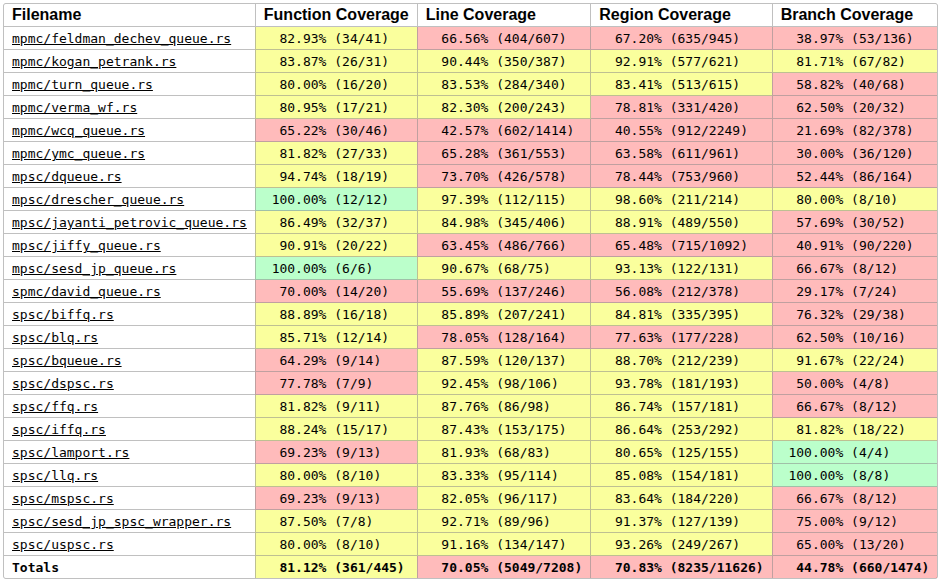
\includegraphics[width=145mm]{images/coverage.png}
    \label{fig:cov}
\end{figure}

    \chapter{Benchmarking and Results}\label{ch:results}
To complete the objective of this thesis, finally a setting needs to be built where these algorithms are used for \ac{IPC} over shared memory. This setting was also used to benchmark the performance of these algorithms to identify the best performing wait-free algorithms that can be used. In the \cite{githubMA} the folder benches includes the setting and benchmark of these algorithms. As seen before, these algorithms were divided into 4 categories, \ac{MPMC}, \ac{MPSC}, \ac{SPMC} and \ac{SPSC}. Therefore, 4 different \ac{IPC} over shared memory settings were built to analyse firstly if all algorithms work as intended and secondly to compare the performance of all algorithms. Even though \ac{SPMC} category only has one algorithm, the built setting was still interesting to check and validate if the algorithm works as intended. After identifying the best algorithm, 3 more settings were built. One setting was to see if the \ac{SPMC} queue or the best performing queues of the other categories would be faster for the \ac{SPSC} category. The same was done for the \ac{MPSC} category by checking if the best \ac{MPMC} queue or the best \ac{MPSC} queue would perform better. Finally, for the \ac{SPMC} category the same was done to check if the best \ac{MPMC} or \ac{SPMC} queue would be better. The best \ac{SPSC} queue could not be tested for higher producer or consumer numbers, since the missing helping structures and missing atomic primitives would lead to deadlocks or inconsistent data. The benchmarks were done on a system with an Intel i7-12700H x86 processor with 14 cores. The benchmarks were implemented with the help of the \texttt{criterion} crate, which is a benchmarking library for Rust. This chapter will show in general how the benchmark settings were implemented to understand the results later.

\section{Benchmark Structure}
All benchmarks follow a consistent architecture to ensure fair comparison between queue implementations. The benchmarks measure the time taken for producers and consumers to exchange a fixed number of items through each queue implementation using \ac{IPC} over shared memory. This section explains the general benchmark structure using the \ac{MPMC} benchmark as a representative example, as the same patterns apply to all queue categories. Not all lines will be explained, but the most important lines will be explained to understand the general structure of the benchmarks. 

\subsection{Benchmark Parameters and Configuration}
Before examining the benchmark implementation details, it is important to understand the benchmark parameters that control the test scenarios. These constants define the scale and scope of the performance measurements, as shown in \cref{lst:bench-constants}.

\begin{lstlisting}[language=Rust, style=boxed, caption={Benchmark configuration constants}, label={lst:bench-constants}]
const ITEMS_PER_PROCESS_TARGET: usize = 170_000;
const PROCESS_COUNTS_TO_TEST: &[(usize, usize)] = &[(1, 1), (2, 2), (4, 4), (6, 6)];
const MAX_BENCH_SPIN_RETRY_ATTEMPTS: usize = 100_000_000_000;
\end{lstlisting}

Line 1 sets the number of items each producer process will generate. The value of 170,000 items provides sufficient workload to measure performance while keeping individual benchmark runs reasonable in duration. Line 2 defines the producer and consumer configurations to test as tuples. The array \texttt{[(1, 1), (2, 2), (4, 4), (6, 6)]} tests symmetric configurations from a single producer and single consumer up to 6 producers and 6 consumers, allowing analysis of scalability. Line 3 sets the maximum spin attempts before considering an operation failed. This large value ensures that wait-free operations have sufficient opportunity to complete.

For other benchmark categories, these constants are adjusted appropriately. For example, the \ac{MPSC} benchmark uses:

\begin{lstlisting}[language=Rust, style=boxed, caption={MPSC-specific configuration}, label={lst:mpsc-constants}]
const ITEMS_PER_PRODUCER_TARGET: usize = 500_000;
const PRODUCER_COUNTS_TO_TEST: &[usize] = &[1, 2, 4, 8, 14];
\end{lstlisting}

The \ac{MPSC} configuration tests up to 14 producers with a single consumer, using more items per producer to ensure the consumer remains busy throughout the benchmark. Similarly, \ac{SPMC} and \ac{SPSC} benchmarks have their own tailored parameters to effectively measure their specific use cases.

\subsection{Benchmark Interface Implementation}
Each queue implementation must provide a uniform interface for benchmarking. This is achieved through a common trait that abstracts the queue-specific operations, as shown in \cref{lst:bench-trait}. The following pop and push traits implement the dequeue and enqueue operations respectively for the queues.

\begin{lstlisting}[language=Rust, style=boxed, caption={Benchmark trait for MPMC queues}, label={lst:bench-trait}]
trait BenchMpmcQueue<T: Send + Clone>: Send + Sync + 'static {
    fn bench_push(&self, item: T, process_id: usize) -> Result<(), ()>;
    fn bench_pop(&self, process_id: usize) -> Result<T, ()>;
    fn bench_is_empty(&self) -> bool;
    fn bench_is_full(&self) -> bool;
}

// Example implementation for YangCrummeyQueue
impl<T: Send + Clone + 'static> BenchMpmcQueue<T> for YangCrummeyQueue<T> {
    fn bench_push(&self, item: T, process_id: usize) -> Result<(), ()> {
        self.enqueue(process_id, item)
    }

    fn bench_pop(&self, process_id: usize) -> Result<T, ()> {
        self.dequeue(process_id)
    }

    fn bench_is_empty(&self) -> bool {
        self.is_empty()
    }

    fn bench_is_full(&self) -> bool {
        false  // YangCrummeyQueue has unbounded capacity
    }
}
\end{lstlisting}

The trait in lines 1 to 6 defines a common interface that all \ac{MPMC} queues must implement. The \texttt{process\_id} parameter in lines 2 and 3 allows queues to distinguish between different processes, which is necessary for some algorithms. Lines 9 to 24 show how the \ac{YMC} queue maps its specific methods to the common interface. The \texttt{bench\_is\_full} method in line 23 returns false for queues with unbounded capacity. This mapping is done for all queues in the respective categories, so that the benchmarks can be run with all queues without changing the benchmark code to compare fairly.

\subsection{Process Synchronisation Infrastructure}
Benchmarking concurrent algorithms requires careful synchronisation to ensure all processes start simultaneously and coordinate their completion for fair comparisons. Two synchronisation structures manage this coordination, as shown in \cref{lst:sync-structures}.

\begin{lstlisting}[language=Rust, style=boxed, caption={Process synchronisation structures}, label={lst:sync-structures}]
#[repr(C)]
struct MpmcStartupSync {
    producers_ready: AtomicU32,
    consumers_ready: AtomicU32,
    go_signal: AtomicBool,
}

impl MpmcStartupSync {
    fn new_in_shm(mem_ptr: *mut u8) -> &'static Self {
        let sync_ptr = mem_ptr as *mut Self;
        unsafe {
            ptr::write(
                sync_ptr,
                Self {
                    producers_ready: AtomicU32::new(0),
                    consumers_ready: AtomicU32::new(0),
                    go_signal: AtomicBool::new(false),
                },
            );
            &*sync_ptr
        }
    }

    fn shared_size() -> usize {
        std::mem::size_of::<Self>()
    }
}

#[repr(C)]
struct MpmcDoneSync {
    producers_done: AtomicU32,
    consumers_done: AtomicU32,
    total_consumed: AtomicUsize,
}
\end{lstlisting}

The \texttt{MpmcStartupSync} structure in lines 1 to 6 coordinates the startup phase. Producers increment \texttt{producers\_ready} in line 3 when ready, consumers increment \texttt{consumers\_ready} in line 4, and all processes wait for \texttt{go\_signal} in line 5 before starting. The \texttt{new\_in\_shm} method in lines 9 to 22 initialises the structure directly in shared memory using placement new. The \texttt{MpmcDoneSync} structure in lines 29 to 34 tracks completion, with \texttt{total\_consumed} in line 33 which is used to verify that no items were lost during the benchmark.

\subsection{Benchmark Execution Framework}

The core benchmark logic is implemented in a generic function that handles process creation, execution, and measurement, as demonstrated in \cref{lst:fork-and-run}.

\begin{lstlisting}[language=Rust, style=boxed, caption={Generic benchmark execution function}, label={lst:fork-and-run}]
fn fork_and_run_mpmc_with_helper<Q, F>(
    queue_init_fn: F,
    num_producers: usize,
    num_consumers: usize,
    items_per_process: usize,
    needs_helper: bool,
) -> Duration
where
    Q: BenchMpmcQueue<usize> + 'static,
    F: FnOnce() -> (&'static Q, *mut u8, usize),
{
    let total_items = num_producers * items_per_process;
    
    // Initialise queue in shared memory
    let (q, q_shm_ptr, q_shm_size) = queue_init_fn();
    
    // Allocate synchronisation structures
    let startup_sync_size = MpmcStartupSync::shared_size();
    let startup_sync_shm_ptr = unsafe { map_shared(startup_sync_size) };
    let startup_sync = MpmcStartupSync::new_in_shm(startup_sync_shm_ptr);
    
    let mut producer_pids = Vec::with_capacity(num_producers);
    let mut consumer_pids = Vec::with_capacity(num_consumers);
    
    // Fork producer processes
    for producer_id in 0..num_producers {
        match unsafe { fork() } {
            Ok(ForkResult::Child) => {
                // Signal ready and wait for go signal
                startup_sync.producers_ready.fetch_add(1, Ordering::AcqRel);
                while !startup_sync.go_signal.load(Ordering::Acquire) {
                    std::hint::spin_loop();
                }
                
                // Produce items
                for i in 0..items_per_process {
                    let item_value = producer_id * items_per_process + i;
                    while q.bench_push(item_value, producer_id).is_err() {
                        std::hint::spin_loop();
                    }
                }
                
                unsafe { libc::_exit(0) };
            }
            Ok(ForkResult::Parent { child }) => {
                producer_pids.push(child);
            }
            Err(e) => panic!("Fork failed: {}", e),
        }
    }
    
    // Wait for all processes to be ready
    while startup_sync.producers_ready.load(Ordering::Acquire) < num_producers as u32
        || startup_sync.consumers_ready.load(Ordering::Acquire) < num_consumers as u32
    {
        std::hint::spin_loop();
    }
    
    // Start timing and signal processes to begin
    let start_time = std::time::Instant::now();
    startup_sync.go_signal.store(true, Ordering::Release);
    
    // Wait for completion
    for pid in producer_pids {
        waitpid(pid, None).expect("waitpid failed");
    }
    
    start_time.elapsed()
}
\end{lstlisting}

The function signature in lines 1 to 10 accepts a queue initialisation function and benchmark parameters. The \texttt{needs\_helper} parameter in line 6 supports queues like Verma's that require a helper thread. Line 15 initialises the queue using the provided function, which returns the queue reference and shared memory details. Lines 26 to 50 show the producer process creation where line 30 signals readiness, lines 31 to 33 implement ensures that every process waits for the go signal, and lines 36 to 41 produce items with retry logic. Lines 53 to 57 ensure all processes are ready before starting. Line 60 captures the start time immediately before signalling processes to begin in line 61. Lines 64 to 66 wait for all producer processes to complete before calculating the elapsed time in line 68.

\subsection{Queue-Specific Benchmark Integration}

Each queue type requires a specific benchmark function that integrates with the Criterion framework, as shown in \cref{lst:queue-benchmark}.

\begin{lstlisting}[language=Rust, style=boxed, caption={Queue-specific benchmark function}, label={lst:queue-benchmark}]
fn bench_yang_crummey(c: &mut Criterion) {
    let mut group = c.benchmark_group("YangCrummeyMPMC_");

    for &(num_prods, num_cons) in PROCESS_COUNTS_TO_TEST {
        let items_per_process = ITEMS_PER_PROCESS_TARGET;
        let total_processes = num_prods + num_cons;

        group.bench_function(
            format!("{}P_{}C", num_prods, num_cons),
            |b: &mut Bencher| {
                b.iter_custom(|_iters| {
                    fork_and_run_mpmc_with_helper::<YangCrummeyQueue<usize>, _>(
                        || {
                            // Calculate required shared memory size
                            let bytes = YangCrummeyQueue::<usize>::shared_size(total_processes);
                            let shm_ptr = unsafe { map_shared(bytes) };
                            
                            // Initialise queue in shared memory
                            let q = unsafe {
                                YangCrummeyQueue::init_in_shared(shm_ptr, total_processes)
                            };
                            
                            (q, shm_ptr, bytes)
                        },
                        num_prods,
                        num_cons,
                        items_per_process,
                        false,  // YangCrummey doesn't need helper
                    )
                })
            },
        );
    }

    group.finish();
}
\end{lstlisting}

Line 2 creates a benchmark group with a descriptive name. Line 4 iterates through different producer/consumer configurations from the constant array \texttt{PROCESS\_COUNTS\_TO\_TEST}. Line 9 formats the benchmark name to indicate the configuration. Lines 11 to 30 use Criterion's \texttt{iter\_custom} method to measure custom timing, as the benchmark itself measures process execution time. The closure in lines 13 to 23 initialises the queue where line 15 calculates the exact shared memory size needed and line 16 allocates the shared memory region. After that lines 19 to 21 initialise the queue at the allocated address.

\subsection{Consumer Process Implementation}
The consumer processes follow a similar pattern but with additional logic to handle termination and verify correctness, as shown in \cref{lst:consumer-process}.

\begin{lstlisting}[language=Rust, style=boxed, caption={Consumer process implementation}, label={lst:consumer-process}]
// Fork consumer processes
for consumer_id in 0..num_consumers {
    match unsafe { fork() } {
        Ok(ForkResult::Child) => {
            startup_sync.consumers_ready.fetch_add(1, Ordering::AcqRel);

            while !startup_sync.go_signal.load(Ordering::Acquire) {
                std::hint::spin_loop();
            }

            let mut consumed_count = 0;
            let target_items = total_items / num_consumers;
            let extra_items = if consumer_id < (total_items % num_consumers) {
                1
            } else {
                0
            };
            let my_target = target_items + extra_items;

            let mut consecutive_empty_checks = 0;
            const MAX_CONSECUTIVE_EMPTY_CHECKS: usize = 40000;

            while consumed_count < my_target {
                match q.bench_pop(num_producers + consumer_id) {
                    Ok(_item) => {
                        consumed_count += 1;
                        consecutive_empty_checks = 0;
                    }
                    Err(_) => {
                        if done_sync.producers_done.load(Ordering::Acquire)
                            == num_producers as u32
                        {
                            consecutive_empty_checks += 1;

                            if consecutive_empty_checks > MAX_CONSECUTIVE_EMPTY_CHECKS {
                                break;  // Queue likely empty
                            }
                        }
                        
                        // Backoff strategy
                        for _ in 0..100 {
                            std::hint::spin_loop();
                        }
                    }
                }
            }

            done_sync
                .total_consumed
                .fetch_add(consumed_count, Ordering::AcqRel);
            done_sync.consumers_done.fetch_add(1, Ordering::AcqRel);

            unsafe { libc::_exit(0) };
        }
        Ok(ForkResult::Parent { child }) => {
            consumer_pids.push(child);
        }
        Err(e) => panic!("Fork failed for consumer: {}", e),
    }
}
\end{lstlisting}

Lines 12 to 18 calculate each consumer's share of items, distributing any remainder among the first consumers. The main consumption loop in lines 23 to 46 implements a termination strategy where lines 25 to 27 reset the empty check counter on successful pop while lines 30 to 38 check if all producers have finished and implement a termination condition. Lines 48 to 51 atomically update the total consumed count for later verification. Line 53 uses \texttt{\_exit} to avoid cleanup that might interfere with shared memory.

\subsection{Validation}
After all producer and consumer processes complete, the benchmark validates that no items were lost or double read during the concurrent operations. This validation is important for ensuring the correctness of each queue implementation under \ac{IPC} scenarios, as shown in \cref{lst:result-validation}.

\begin{lstlisting}[language=Rust, style=boxed, caption={Post-benchmark validation of results}, label={lst:result-validation}]
// Wait for all processes to complete
for pid in producer_pids {
    waitpid(pid, None).expect("waitpid for producer failed");
}

for pid in consumer_pids {
    waitpid(pid, None).expect("waitpid for consumer failed");
}

let duration = start_time.elapsed();

// Validate that all items were consumed
let total_consumed = done_sync.total_consumed.load(Ordering::Acquire);

if total_consumed != total_items {
    eprintln!(
        "Warning (MPMC): Total consumed {}/{} items. Q: {}, Prods: {}, Cons: {}",
        total_consumed,
        total_items,
        std::any::type_name::<Q>(),
        num_producers,
        num_consumers
    );
}

// Clean up shared memory regions
unsafe {
    if !q_shm_ptr.is_null() {
        unmap_shared(q_shm_ptr, q_shm_size);
    }
    unmap_shared(startup_sync_shm_ptr, startup_sync_size);
    unmap_shared(done_sync_shm_ptr, done_sync_size);
}

duration
\end{lstlisting}

Lines 2 to 8 wait for all processes to complete before proceeding with validation. After that line 13 atomically reads the total number of items consumed across all consumer processes. The validation check in lines 15 to 24 compares the consumed count against the expected total. If items are missing, line 17 prints a detailed warning that includes the actual versus expected counts in line 18, the queue type name in line 20, and the producer and consumer configuration in lines 21 and 22. This warning helps identify queue implementations that may lose items under high contention or have synchronisation issues and to verify that the queue operates correctly under concurrent access, if the warning does not appear.

\subsection{Benchmark Configuration}
The benchmarks use Criterion's configuration options to ensure reliable measurements, as shown in \cref{lst:criterion-config}.

\begin{lstlisting}[language=Rust, style=boxed, caption={Criterion benchmark configuration}, label={lst:criterion-config}]
fn custom_criterion() -> Criterion {
    Criterion::default()
        .warm_up_time(Duration::from_secs(1))
        .measurement_time(Duration::from_secs(4200))
        .sample_size(500)
}

criterion_group! {
    name = benches;
    config = custom_criterion();
    targets =
        bench_wcq_queue,
        bench_turn_queue,
        bench_kogan_petrank_queue,
        bench_yang_crummey
}

criterion_main!(benches);
\end{lstlisting}

Line 3 sets a 1-second warm-up period to stabilise system state. Line 4 configures 4200 seconds of measurement time per benchmark. Line 5 sets 500 samples, as each sample involves creating multiple processes and produce and consume a set number of items. Lines 8 to 16 define the benchmark group with all queue implementations to test.

The same benchmark structure is applied to all benchmarks with appropriate modifications to the number of producers and consumers. This consistent approach ensures fair comparison across all implementations while accurately measuring their performance characteristics under \ac{IPC} scenarios.

\section{Benchmark Results}
The benchmark results are presented for each queue category, followed by cross-category comparisons to determine the optimal wait-free data structure for different contention scenarios. All measurements represent the mean execution time in microseconds ($\mu$s) for completing the configured workload across multiple samples. In every bench 500 samples were taken to obtain sufficient results to compare the performance. The amount of data produced and consumed was always different for each category. The queues inside each category were always tested with the same amount of data to ensure fair comparison. The amount of items used for each category is shown in the respective subsections.

\subsection{\acf{SPSC} Queue Performance}
The \ac{SPSC} benchmarks evaluated 11 different queue implementations with 35,000,000 items to ensure sufficient workload for accurate measurement. As shown in \cref{tab:spsc-results}, the \ac{BLQ} achieved the best performance with a mean execution time of 65,199.6 $\mu$s.

\begin{table}[htb]
\centering
\caption{\ac{SPSC} Queue Performance Results (35,000,000 items)}
\label{tab:spsc-results}
\begin{tabular}{@{}lrr@{}}
\toprule
Queue Implementation & Mean Time ($\mu$s) & Relative Performance \\
\midrule
\ac{BLQ} & 65,199.6 & 1.00x \\
\ac{IFFQ} & 124,149.9 & 1.90x \\
\ac{LLQ} & 147,800.2 & 2.27x \\
\ac{BIFFQ} & 159,429.6 & 2.45x \\
\ac{FFQ} & 203,053.4 & 3.11x \\
\ac{mSPSC} & 331,283.6 & 5.08x \\
\ac{uSPSC} & 418,840.0 & 6.42x \\
\ac{JPQ}'s \ac{SPSC} Variant & 626,541.9 & 9.61x \\
Lamport's Queue & 957,312.6 & 14.68x \\
B-Queue & 1,552,513.1 & 23.81x \\
\ac{dSPSC} & 2,413,354.7 & 37.02x \\
\bottomrule
\end{tabular}
\end{table}

The results reveal that the cache-aware algorithms (\ac{BLQ}, \ac{IFFQ}, \ac{LLQ}, \ac{BIFFQ}) are all faster than the other approaches, demonstrating the importance of cache optimisation. The \ac{BLQ}'s superior performance can be attributed to its additional batching mechanism, which amortises synchronisation costs across multiple operations while maintaining cache locality.

Notably, the dynamic allocation-based queues (\ac{dSPSC}, \ac{uSPSC}) showed worse performance, with \ac{dSPSC} being 37 times slower than \ac{BLQ}. This overhead stems from the memory pool management required for shared memory compatibility, as discussed in \cref{ch:implementation}.

\begin{figure}[htb]
\centering
\caption{Violin plot showing the distribution of execution times for \ac{SPSC} queue implementations and 35,000,000 total items)}
\label{fig:spsc-violin}
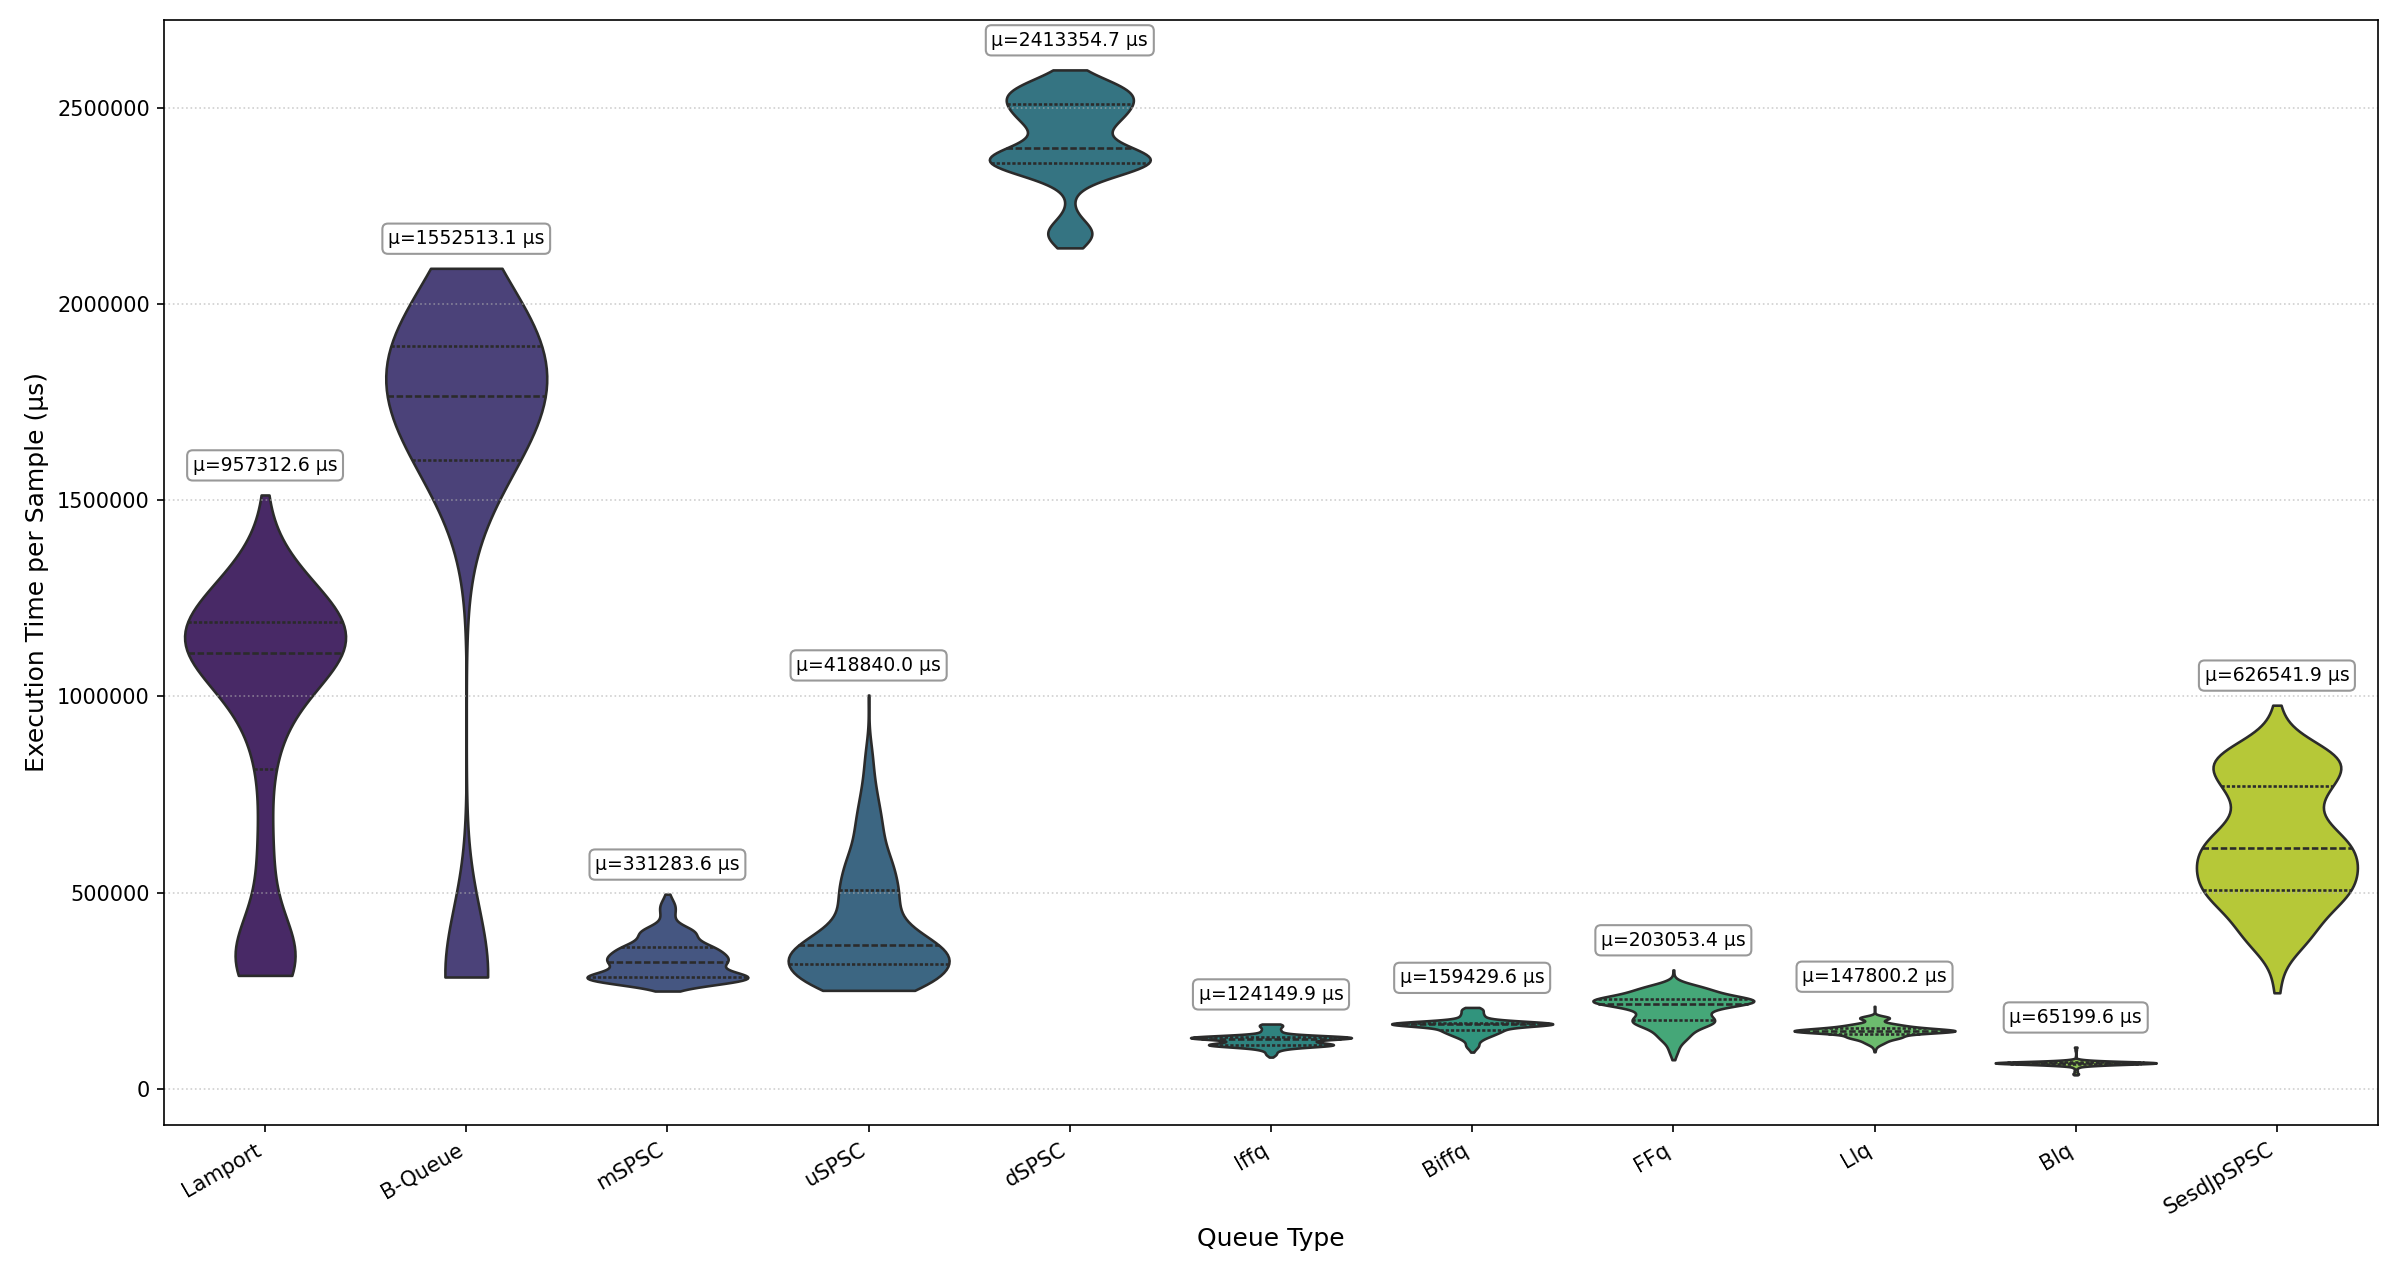
\includegraphics[width=\textwidth]{images/results/spsc_queue_performance_violin_test.png}
\end{figure}

The violin plot in \cref{fig:spsc-violin} illustrates the distribution of execution times across all SPSC implementations. It can be observed that the Lamport queue has no consistent performance with greatly varying results. It often achieves great execution times, but also often bad execution times. This is probably because of bad cache design of the queue that was talked about in \cref{alg:lamport-queue}. The \ac{BLQ} on the other hand shows not only the lowest median execution time but also the most consistent performance with minimal variance, which is an important trait for designing hard timing constraints for \ac{HRTS}. 

\subsection{\acf{MPSC} Queue Performance}
For \ac{MPSC} scenarios, four queue implementations were tested with varying producer counts from 1 to 14, each producer generating 500,000 items. \cref{tab:mpsc-results} presents the mean performance across different producer configurations, which is visualised in \cref{fig:mpsc-mean-performance}. DQueue with a mean execution time of 13,967.2 $\mu$s for 1 producer, 29,039.9 $\mu$s for 2 producers, and scaling up to 323,126.2 $\mu$s for 14 producers, outperformed all other implementations.

\begin{table}[htb]
\centering
\caption{\ac{MPSC} Queue Performance Results (500,000 items per producer)}
\label{tab:mpsc-results}
\begin{tabular}{@{}lrrrrr@{}}
\toprule
Queue & 1P & 2P & 4P & 8P & 14P \\
\midrule
DQueue & 13,967.2 & 29,039.9 & 72,894.1 & 170,676.4 & 323,126.2 \\
Drescher & 22,932.0 & 89,353.0 & 189,703.0 & 434,820.2 & 955,047.8 \\
Jiffy & 32,280.3 & 62,159.1 & 126,199.3 & 276,401.5 & 538,978.2 \\
\ac{JPQ}'s \ac{MPSC} Variant & 94,912.5 & 252,959.1 & 648,641.6 & 2,191,529.2 & 4,548,422.3 \\
\bottomrule
\end{tabular}
\end{table}

\begin{figure}[htb]
\centering
\caption{Mean execution time of MPSC queue implementations as producer count increases}
\label{fig:mpsc-mean-performance}
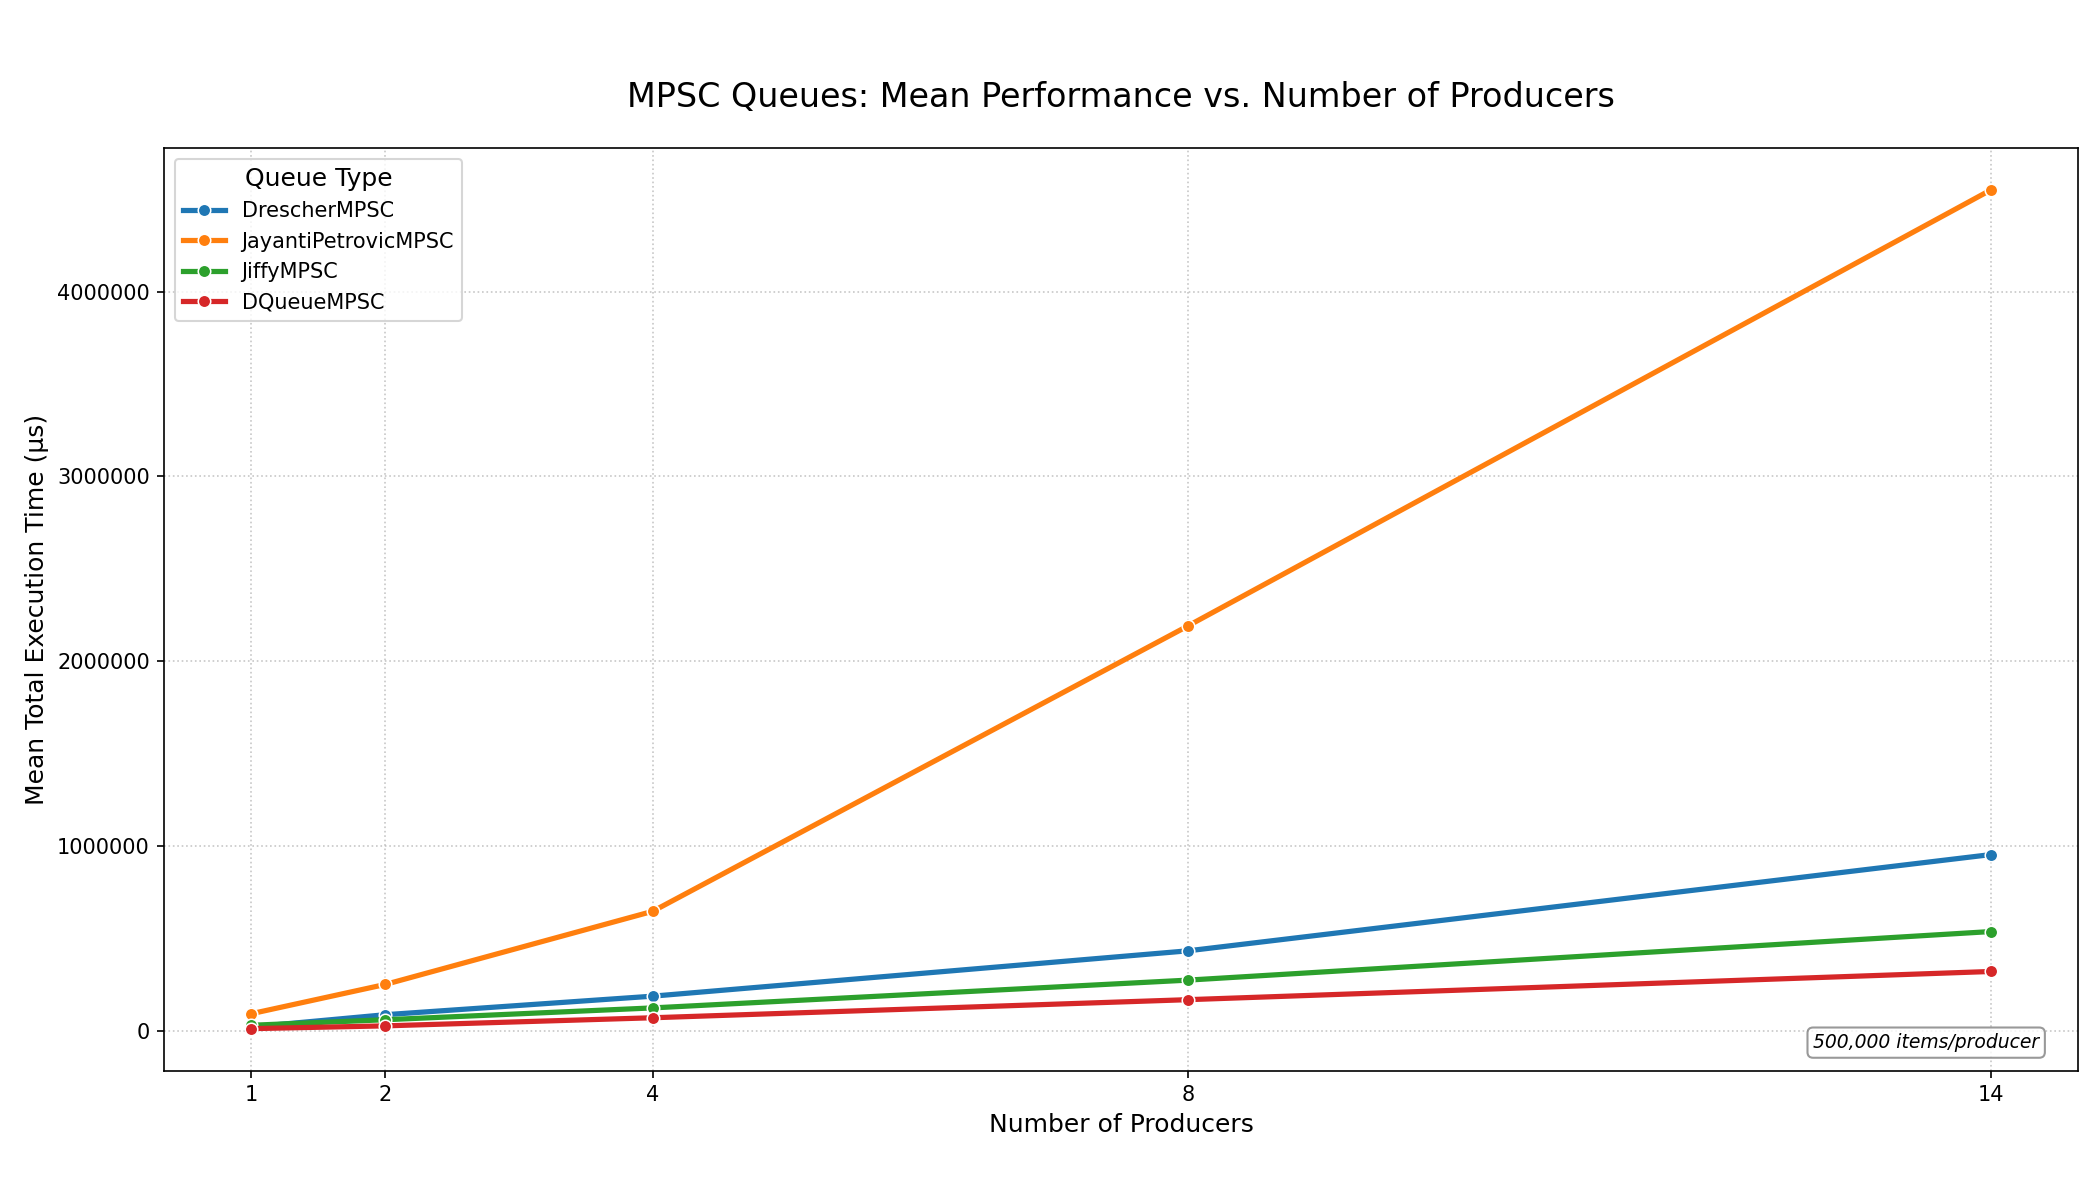
\includegraphics[width=\textwidth]{images/results/mpsc_mean_performance_vs_producers.png}
\end{figure}

DQueue had the best performance overall as producer count increased. The DQueue's local buffering mechanism effectively reduces contention by minimising synchronisation operations, as each producer accumulates items locally before batch-writing to the shared queue.

The \ac{JPQ}, despite its theoretical $O(\log n)$ complexity, showed poor practical performance. This is due to the overhead of maintaining the binary tree structure for timestamp propagation. This highlights the gap between theoretical complexity and real-world performance in concurrent data structures.

\begin{figure}[htb]
\centering
\caption{Violin plot showing the distribution of execution times for MPSC queue implementations with 14 producers and 1 consumer and 7,000,000 total items}
\label{fig:mpsc-violin-14p}
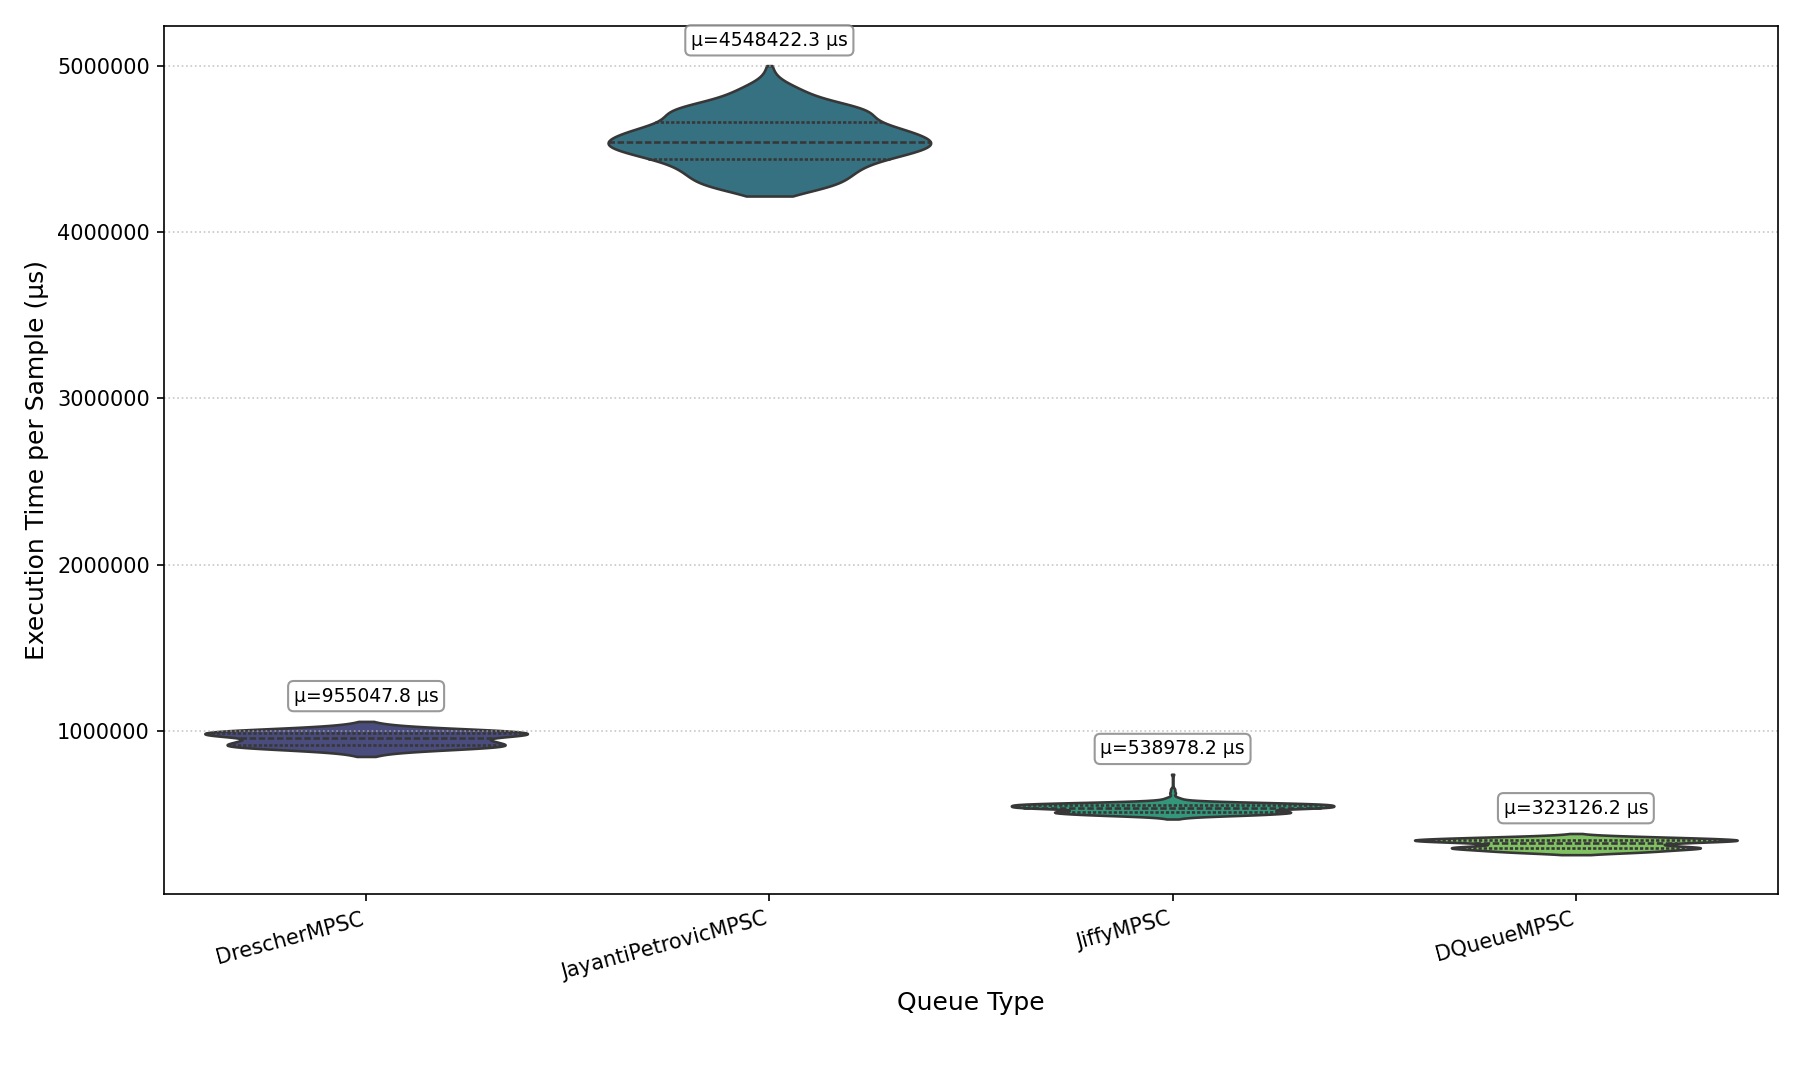
\includegraphics[width=\textwidth]{images/results/mpsc_performance_violin_14_producers.png}
\end{figure}

\cref{fig:mpsc-violin-14p} shows the performance distribution under maximum contention (14 producers). DQueue maintains a tight distribution even under high producer contention, which is also the case for lesser producer counts as seen in \cref{fig:mpsc-violin-1p,fig:mpsc-violin-2p,fig:mpsc-violin-4p,fig:mpsc-violin-8p}. This shows that DQueue's design is ensuring consistent enough performance to design hard timing constraints for \ac{HRTS}.

\subsection{\acf{SPMC} Queue Performance}
Only one native \ac{SPMC} implementation was available. So no performance comparison was made with another \ac{SPMC} queue. What was done is comparing the performance of the David queue with the best performing \ac{MPMC} queue in a \ac{SPMC} benchmark setting, to see if maybe the best performing \ac{MPMC} queue would be even better in a \ac{SPMC} setting than a native \ac{SPMC} queue. This can be seen in \cref{subsubsec:cross-spmc}.

\subsection{\acf{MPMC} Queue Performance}
The \ac{MPMC} category included six implementations tested with symmetric producer-consumer configurations. Each producer generated 170,000 items. \cref{tab:mpmc-results} shows the mean performance across different producer-consumer configurations, which is again visualised as seen in \cref{fig:mpmc-mean-performance}.

\begin{table}[htb]
\centering
\caption{\ac{MPMC} Queue Performance Results (170,000 items per producer)}
\label{tab:mpmc-results}
\begin{tabular}{@{}lrrrr@{}}
\toprule
Queue & 1P/1C & 2P/2C & 4P/4C & 6P/6C \\
\midrule
\ac{YMC} & 72,910.8 & 72,547.6 & 101,541.4 & 121,477.9 \\
Verma & 45,690.9 & 73,042.7 & 153,716.8 & 229,763.6 \\
FeldmanDechev & 90,956.0 & 100,893.5 & 150,636.2 & 278,037.7 \\
TurnQueue & 100,150.3 & 173,204.2 & 510,697.0 & 971,945.7 \\
KoganPetrank & 174,502.6 & 285,645.9 & 896,079.8 & 1,574,045.2 \\
\ac{wCQ} & 233,996.9 & 248,234.3 & 350,401.3 & 518,476.6 \\
\bottomrule
\end{tabular}
\end{table}

\begin{figure}[htb]
\centering
\caption{Mean execution time of MPMC queue implementations as process count increases}
\label{fig:mpmc-mean-performance}
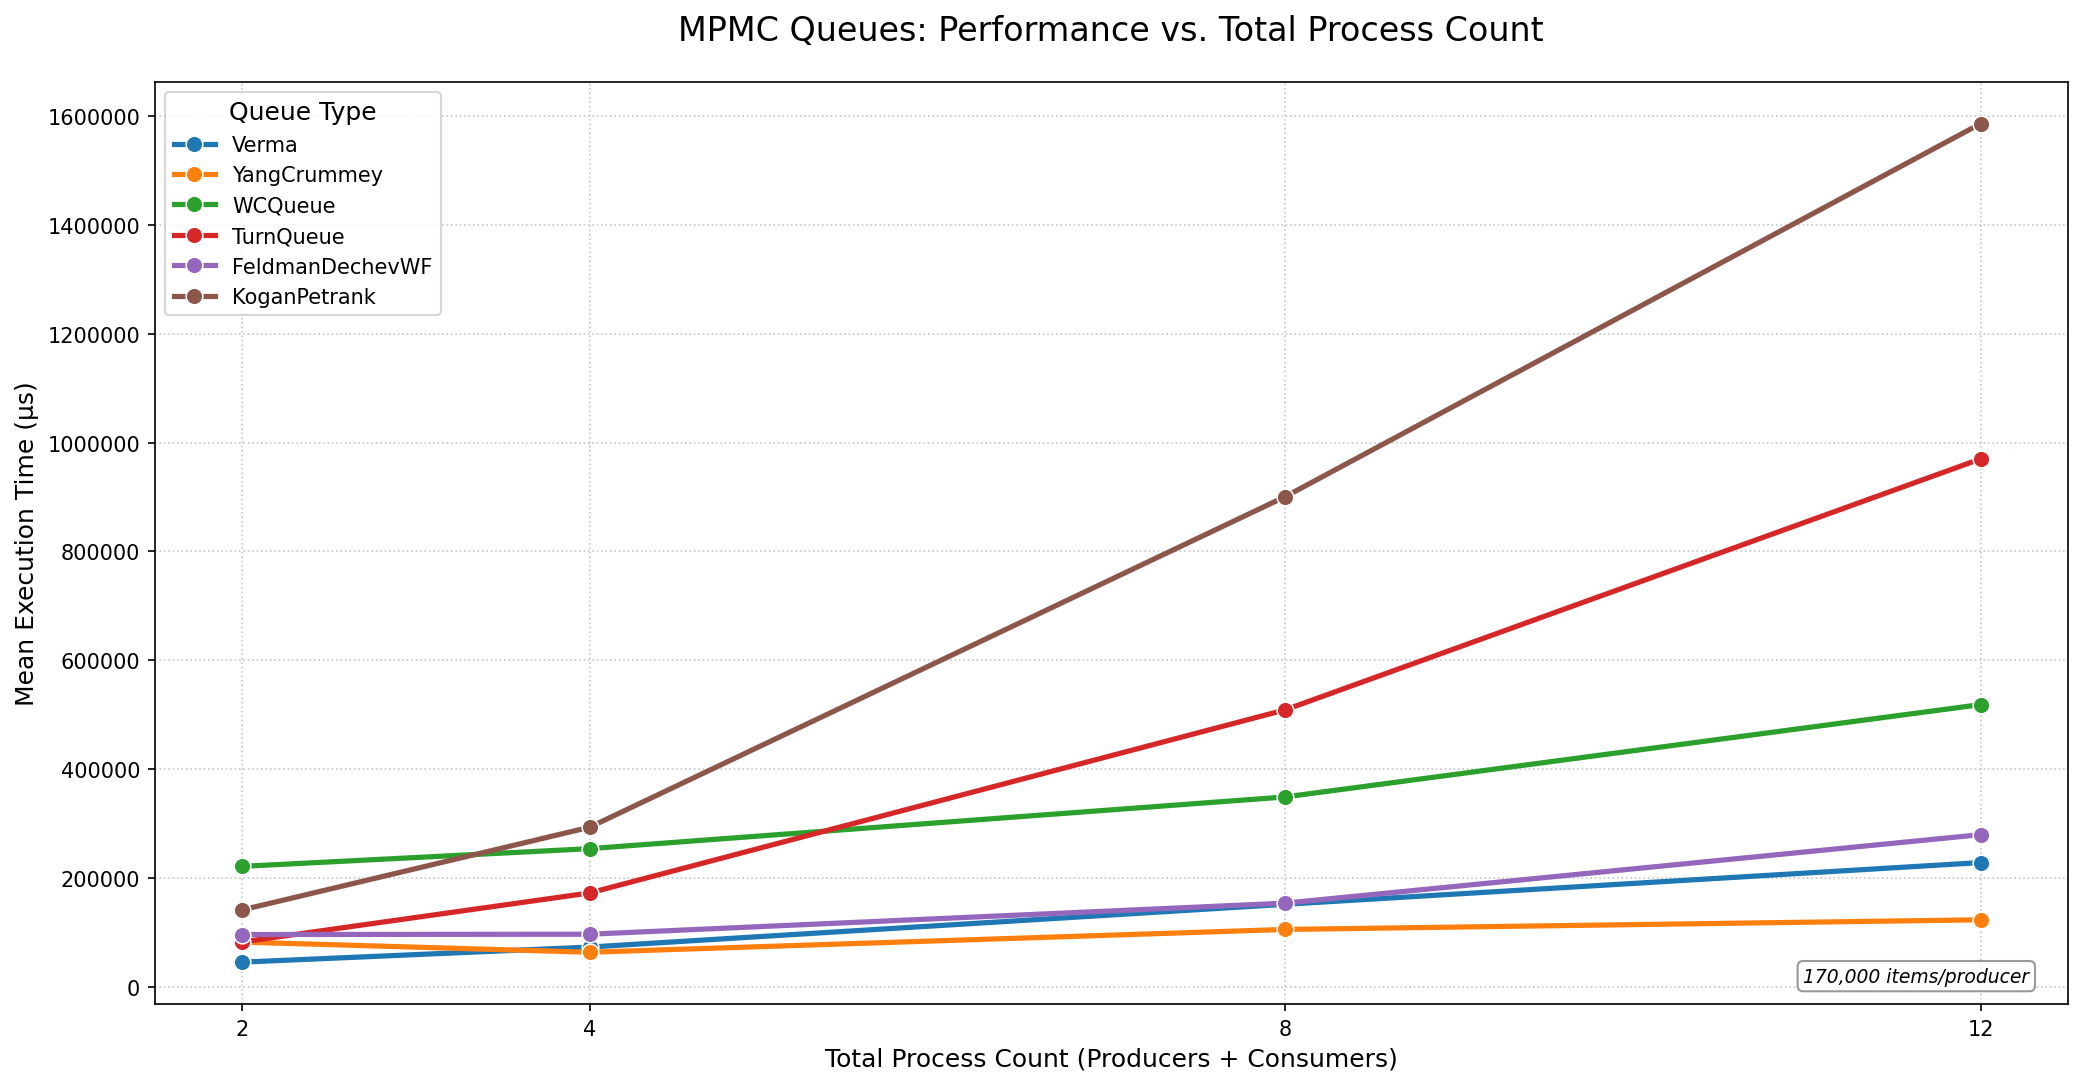
\includegraphics[width=\textwidth]{images/results/mpmc_mean_performance_vs_processes.png}
\end{figure}

The \ac{YMC} queue achieved the best overall performance with 72,910.8 $\mu$s for 1 producer and 1 consumer, 72,547.6 $\mu$s for 2 producers and 2 consumers, and scaling to 121,477.9 $\mu$s for 6 producers and 6 consumers. Its performance remained relatively stable across different configurations, demonstrating its efficiency in handling multiple producers and consumers.

What can be observed is that the Verma queue has better performance in the 1P/1C case with a mean performance of 45,690.9 $\mu$s than \ac{YMC}. The reason for that is most probably because even in the 1P/1C case there is still an active dedicated helper thread that is used to help the producer and consumer processes.

\begin{figure}[htb]
\centering
\caption{Violin plot showing the distribution of execution times for MPMC queue implementations with 6 producers and 6 consumers and 1,020,000 total items}
\label{fig:mpmc-violin-6p6c}
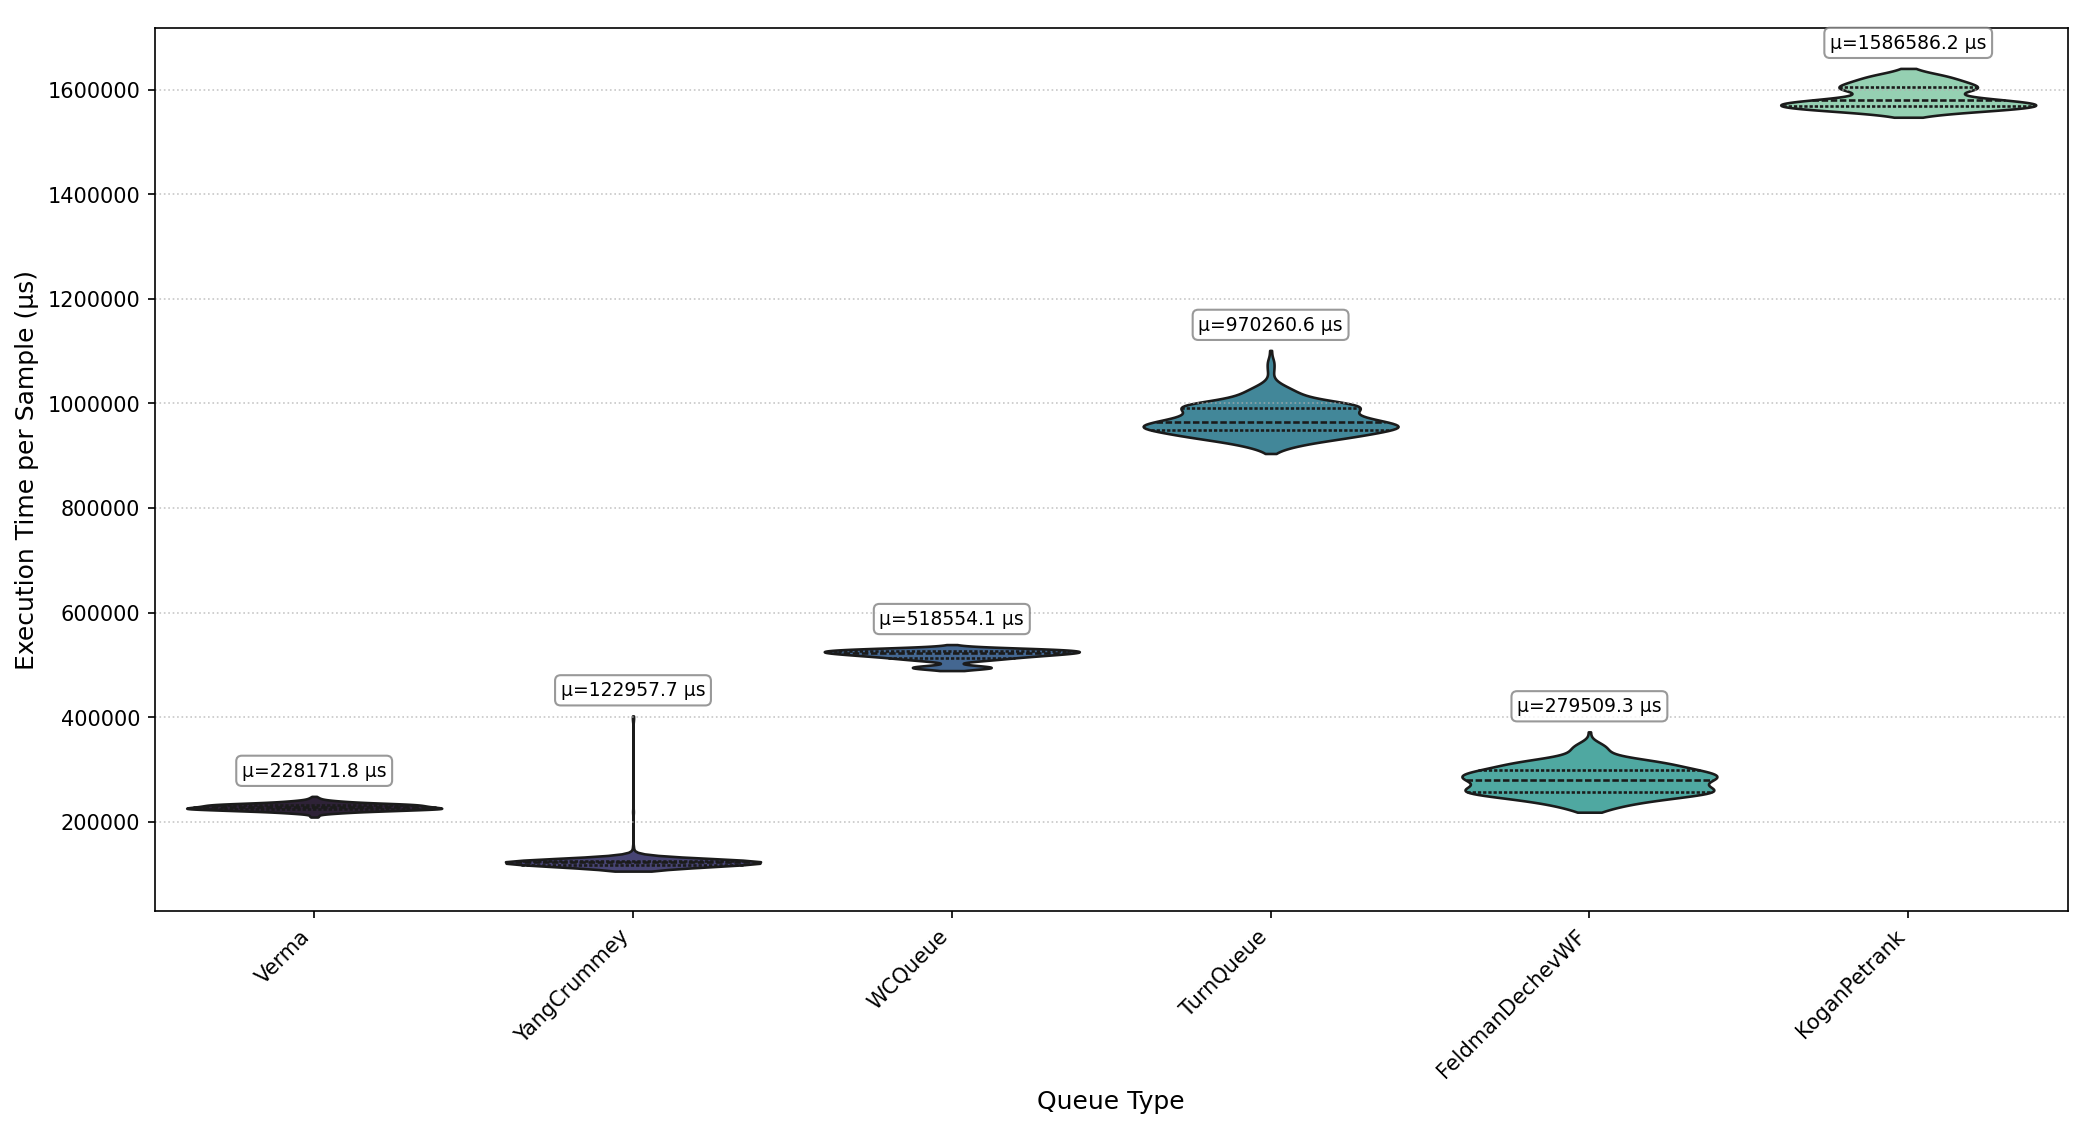
\includegraphics[width=\textwidth]{images/results/mpmc_performance_violin_6P_6C.png}
\end{figure}

\cref{fig:mpmc-violin-6p6c} illustrates the performance distribution under symmetric high contention (6P/6C). The \ac{YMC} queue demonstrates that its performance stays consistent with minimal variance, even in lesser producer and consumer counts as seen in \cref{fig:mpmc-violin-2p2c,fig:mpmc-violin-4p4c}, indicating predictable performance beneficial to define tight timing constraints for \ac{HRTS}. The only exception is the 1P/1C case, where the performance distribution is more spread out, as seen in \cref{fig:mpmc-violin-1p1c} indicating that \ac{YMC} is not as optimised for low contention scenarios as it is for high contention scenarios. The Verma queue has consistent performance over all process counts, but with a higher mean execution time than \ac{YMC}. So for \ac{HRTS} which requires predictability, Verma queue could be a better choice even though it is not the fastest queue in the \ac{MPMC} category.

\subsection{Cross-Category Performance Comparison}
To determine whether specialised queues for each contention category are necessary, cross-category benchmarks were conducted comparing the best performers from each category against queues from other categories. The specialised queues for their respective contention scenarios were called native in each cross-category benchmark. The results are summarised in the following subsections.


\subsubsection{Best Queue for \ac{SPSC} Scenarios}
\cref{tab:best-spsc} compares the native \ac{SPSC} winner (\ac{BLQ}) against the best queues from other categories operating in \ac{SPSC} mode with 300,000 items.

\begin{table}[htb]
\centering
\caption{Cross-Category Performance in \ac{SPSC} Configuration (300,000 items)}
\label{tab:best-spsc}
\begin{tabular}{@{}lrr@{}}
\toprule
Queue (Category) & Mean Time ($\mu$s) & Relative to \ac{BLQ} \\
\midrule
\ac{BLQ} (Native SPSC) & 3,625.7 & 1.00x \\
DQueue (MPSC as SPSC) & 7,638.9 & 2.11x \\
David (SPMC as SPSC) & 21,207.3 & 5.85x \\
\ac{YMC} (MPMC as SPSC) & 36,170.9 & 9.98x \\
\bottomrule
\end{tabular}
\end{table}

The native \ac{SPSC} queue with a mean performance of $3,625.7\mu$s outperformed all others, being 2.11x faster than DQueue and nearly 10x faster than \ac{YMC}. This demonstrates that specialised \ac{SPSC} algorithms provide benefits when contention is limited to a single producer and consumer pair. \cref{fig:cross-spsc-violin} visualises this again.

\begin{figure}[htb]
\centering
\caption{Violin plot showing performance distribution of different queue categories operating in an \ac{SPSC} setting with 300,000 total items}
\label{fig:cross-spsc-violin}
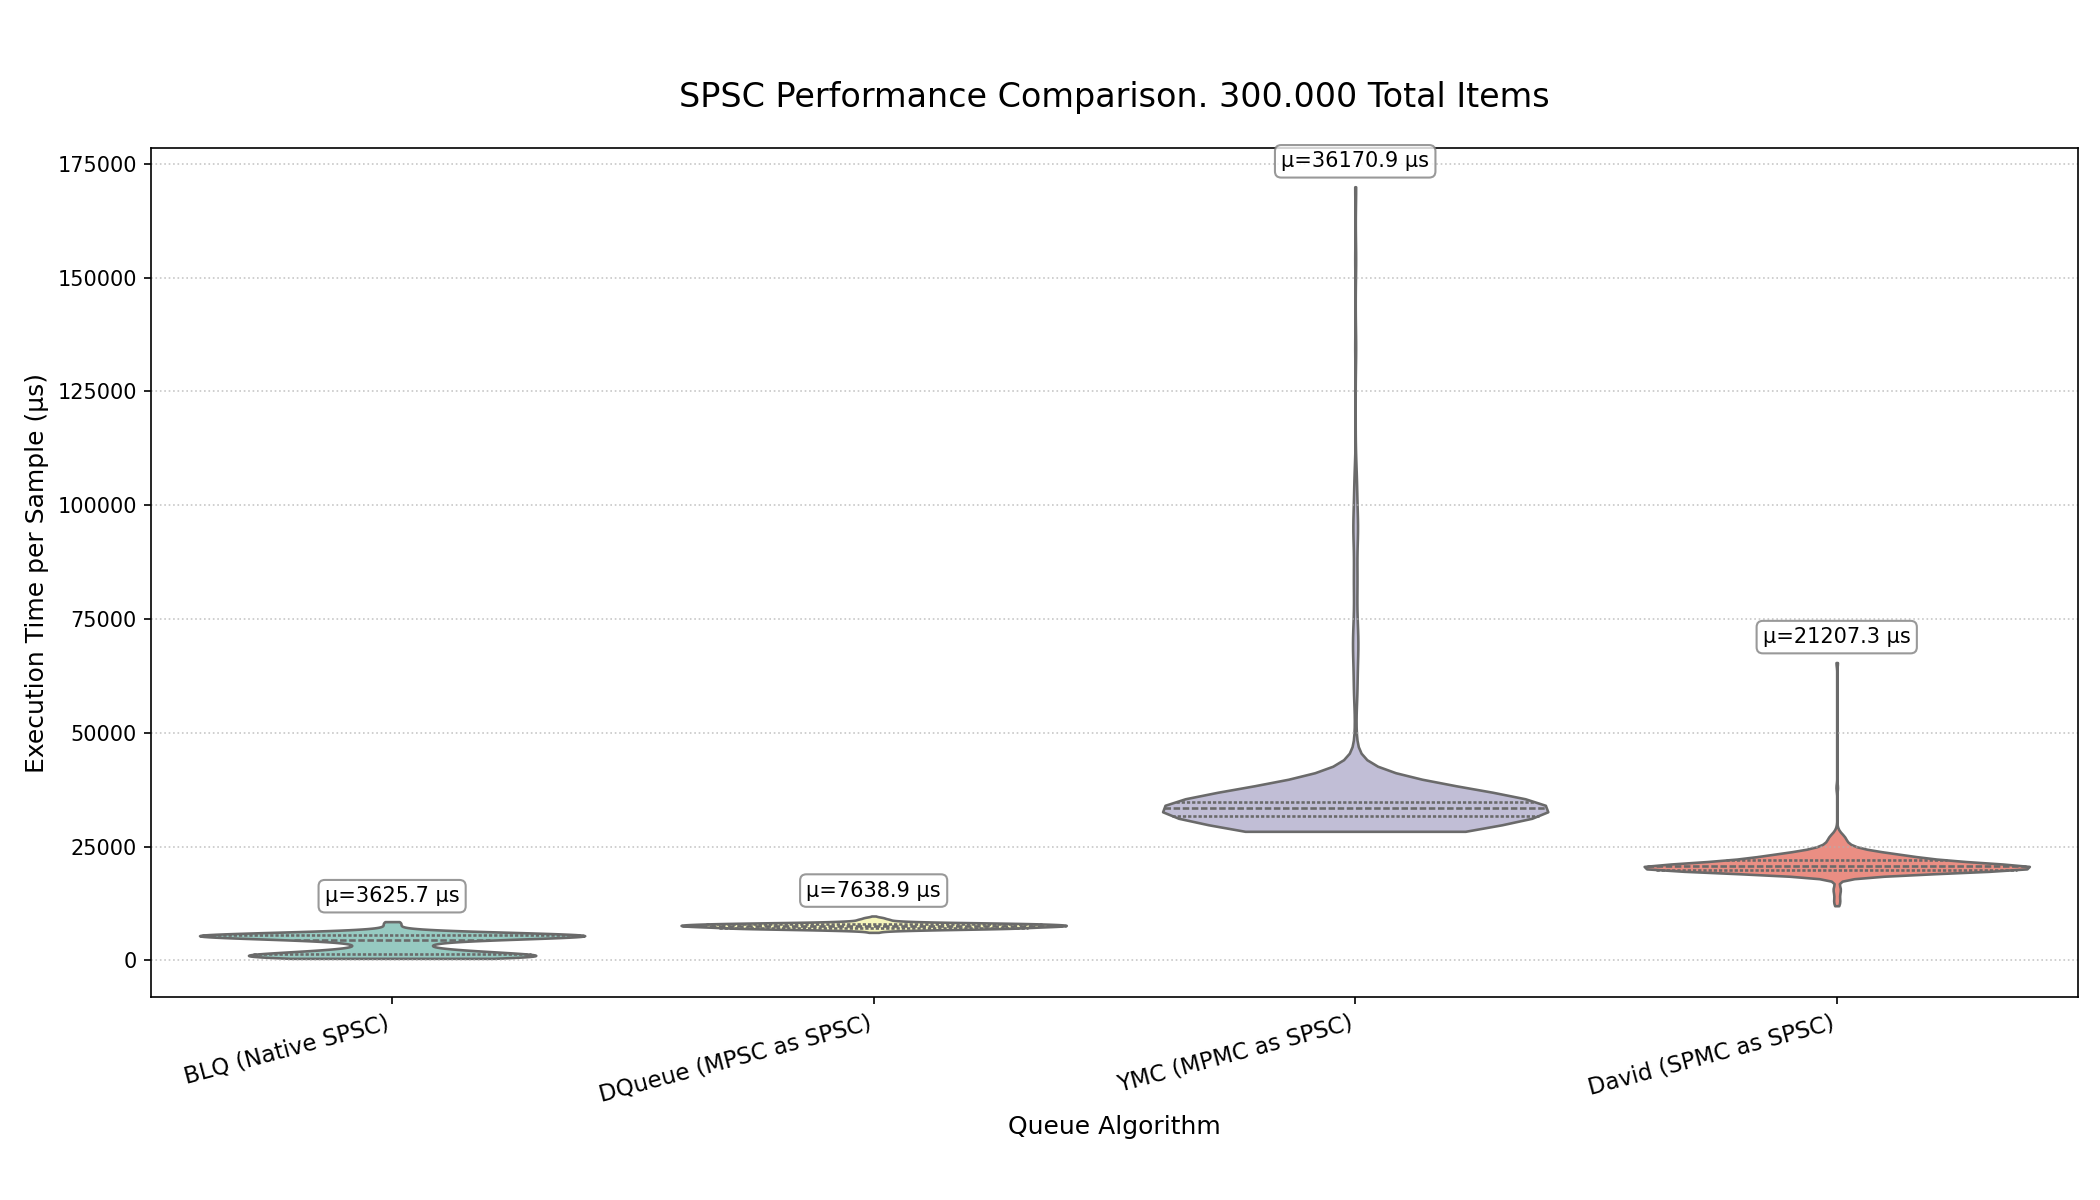
\includegraphics[width=\textwidth]{images/results/best_algorithms_in_spsc_performance.png}
\end{figure}

\subsubsection{Best Queue for \ac{MPSC} Scenarios}
Comparing the native \ac{MPSC} winner DQueue against \ac{YMC} operating in an \ac{MPSC} setting reveals similar patterns, as shown in \cref{tab:best-mpsc} visualised in \cref{fig:cross-mpsc-mean}.

\begin{table}[htb]
\centering
\caption{Cross-Category Performance in \ac{MPSC} Configuration (100,000 items per producer)}
\label{tab:best-mpsc}
\begin{tabular}{@{}lrrr@{}}
\toprule
Producers & DQueue (Native \ac{MPSC}) & \ac{YMC} (as \ac{MPSC}) & Relative to DQueue \\
& Time ($\mu$s) & Time ($\mu$s) & \\
\midrule
1 & 2,102.7 & 13,075.6 & 6.22x \\
2 & 7,081.9 & 19,650.4 & 2.77x \\
4 & 16,588.1 & 39,848.3 & 2.40x \\
8 & 36,197.5 & 84,092.5 & 2.32x \\
14 & 72,788.4 & 168,854.4 & 2.32x \\
\bottomrule
\end{tabular}
\end{table}

DQueue outperformed \ac{YMC} across all producer counts, with the performance gap decreasing from 6.22x at 1 producer to 2.32x at 14 producers. The native \ac{MPSC} implementation maintains its advantage due to its optimised local buffering mechanism that reduces synchronisation overhead. \ac{YMC} has overhead from its additional consumer synchronisation mechanisms, which are not needed in an \ac{MPSC} setting.

\begin{figure}[htb]
\centering
\caption{Mean execution time comparison of DQueue (native MPSC) vs YMC (as MPSC) across different producer counts}
\label{fig:cross-mpsc-mean}
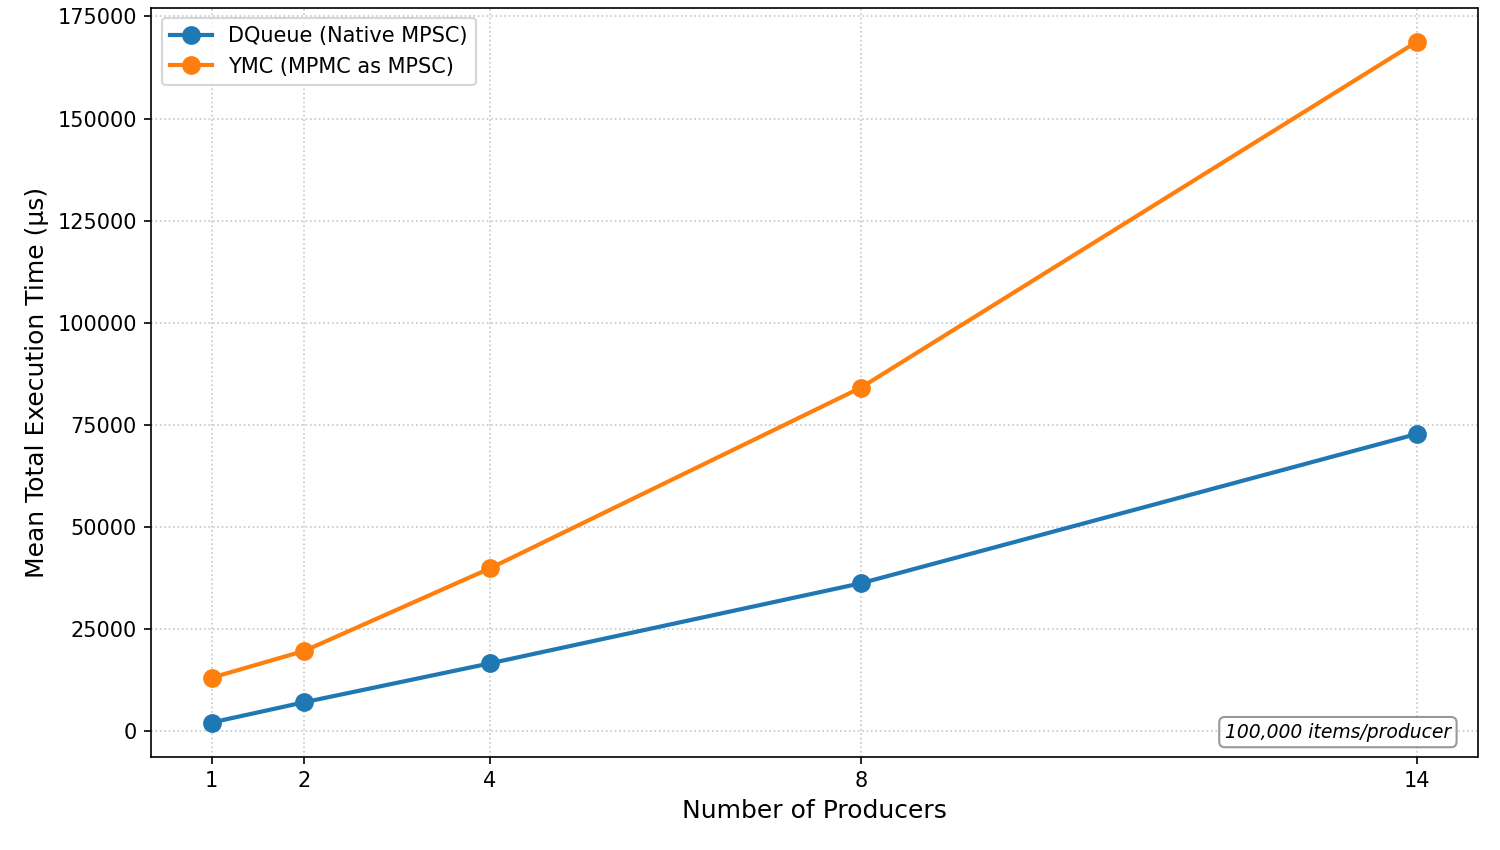
\includegraphics[width=\textwidth]{images/results/best_in_mpsc_mean_performance_vs_producers.png}
\end{figure}

\begin{figure}[htb]
\centering
\caption{Violin plot showing the distribution of execution times for cross-category MPSC comparison with 14 producers and 1 consumer and 1,400,000 total items}
\label{fig:cross-mpsc-violin-14p}
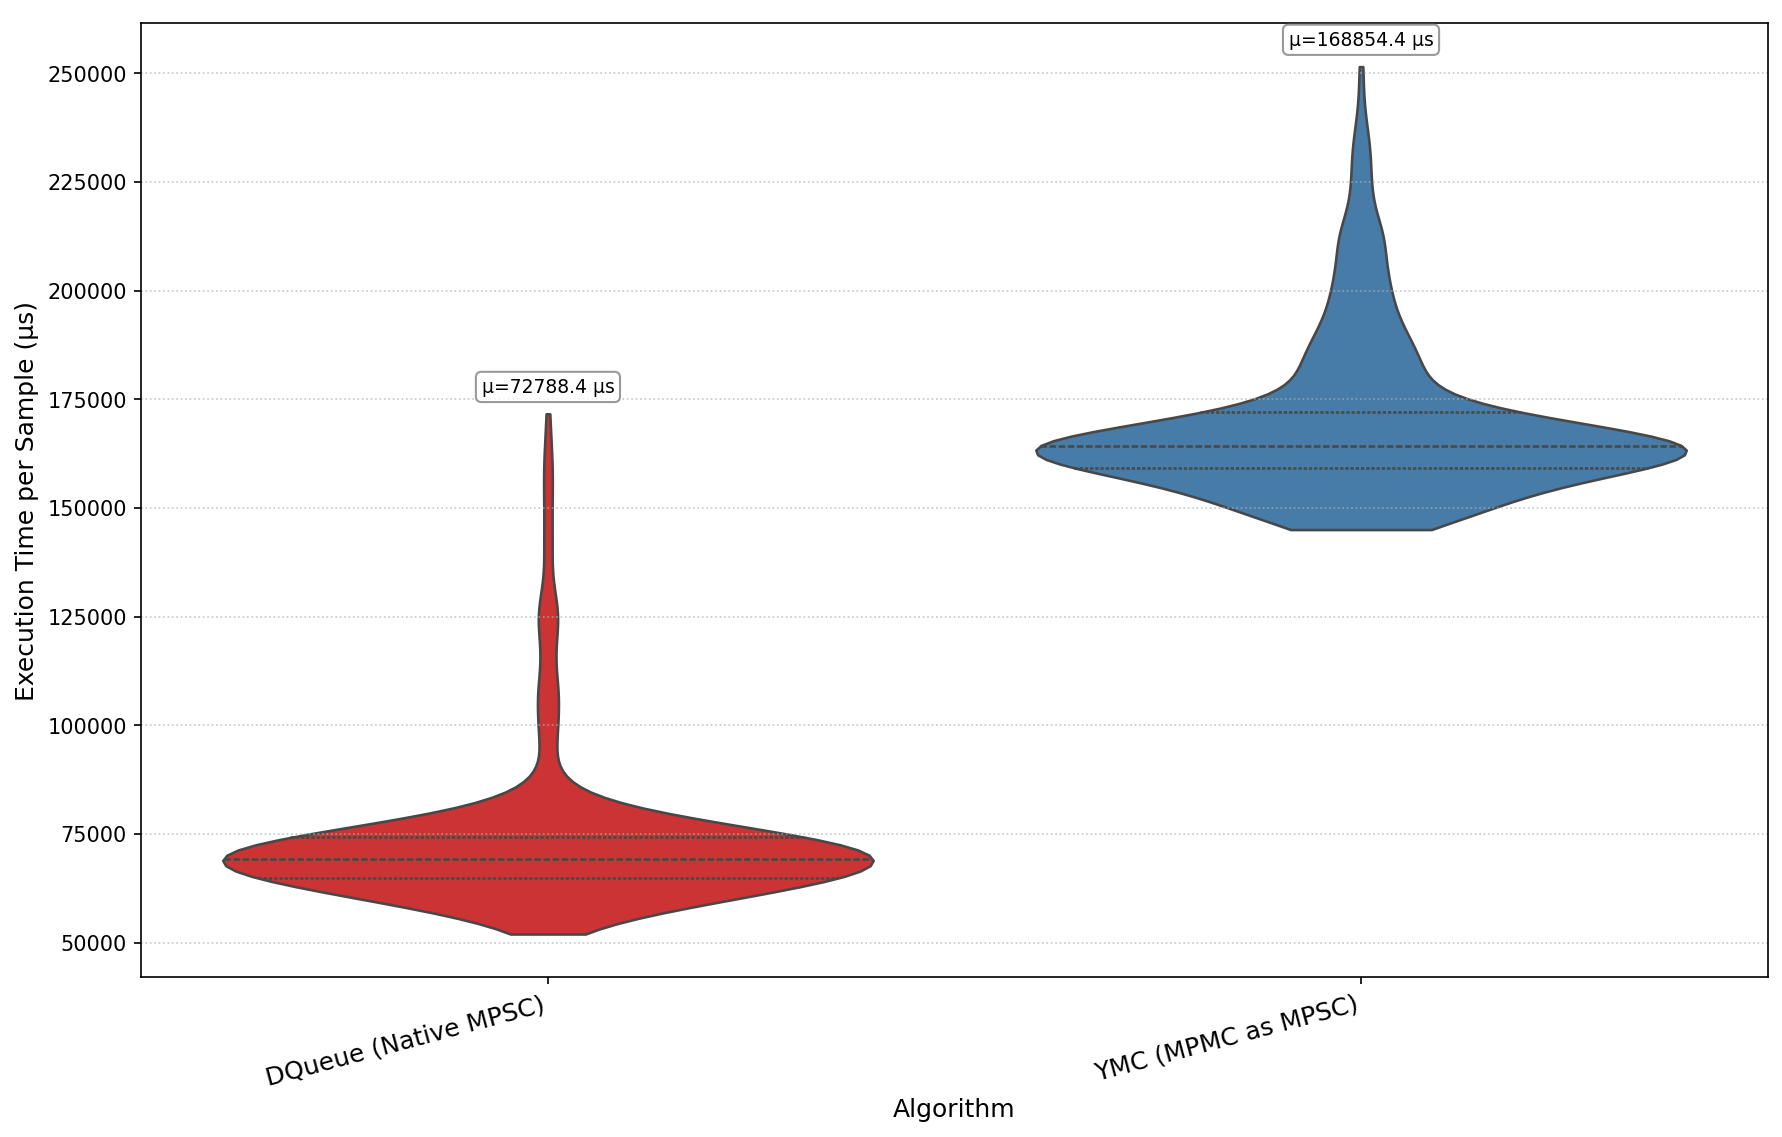
\includegraphics[width=\textwidth]{images/results/best_in_mpsc_performance_violin_14P1C.png}
\end{figure}

\cref{fig:cross-mpsc-violin-14p} illustrates the performance distribution comparison between DQueue (native MPSC) and \ac{YMC} (operating as MPSC) under maximum producer contention (14 producers). DQueue shows slightly better consistency whilst performing faster than \ac{YMC}, showing that also in \ac{MPSC} settings specialised queues are better than more general \ac{MPMC} queues. The same goes too for lesser producer counts as seen in \cref{fig:cross-mpsc-violin-1p,fig:cross-mpsc-violin-2p,fig:cross-mpsc-violin-4p,fig:cross-mpsc-violin-8p}.

\subsubsection{Best Queue for \ac{SPMC} Scenarios}\label{subsubsec:cross-spmc}
The native \ac{SPMC} implementation (David) was compared against \ac{YMC} in \ac{SPMC} mode, as presented in \cref{tab:best-spmc}.

\begin{table}[htb]
\centering
\caption{Cross-Category Performance in \ac{SPMC} Configuration (100,000 items per consumer)}
\label{tab:best-spmc}
\begin{tabular}{@{}lrrr@{}}
\toprule
Consumers & David (Native \ac{SPMC}) & \ac{YMC} (as \ac{SPMC}) & Relative to David \\
& Time ($\mu$s) & Time ($\mu$s) & \\
\midrule
1 & 2,754.4 & 16,696.0 & 6.06x \\
2 & 8,222.4 & 24,220.6 & 2.95x \\
4 & 17,243.9 & 44,368.2 & 2.57x \\
8 & 37,756.0 & 96,410.1 & 2.55x \\
14 & 71,305.7 & 225,931.3 & 3.17x \\
\bottomrule
\end{tabular}
\end{table}

Similar to the \ac{MPSC} results, the specialised David queue significantly outperformed \ac{YMC}, maintaining a 2.5-6x performance advantage across different consumer counts. The native \ac{SPMC} algorithm's two-dimensional array design with row jumping proves to be faster than the \ac{MPMC} approach.

\begin{figure}[htb]
\centering
\caption{Violin plot showing the distribution of execution times for \ac{SPMC} implementations with 1 producer and 14 consumers and 1,400,000 total items}
\label{fig:spmc-violin-14c}
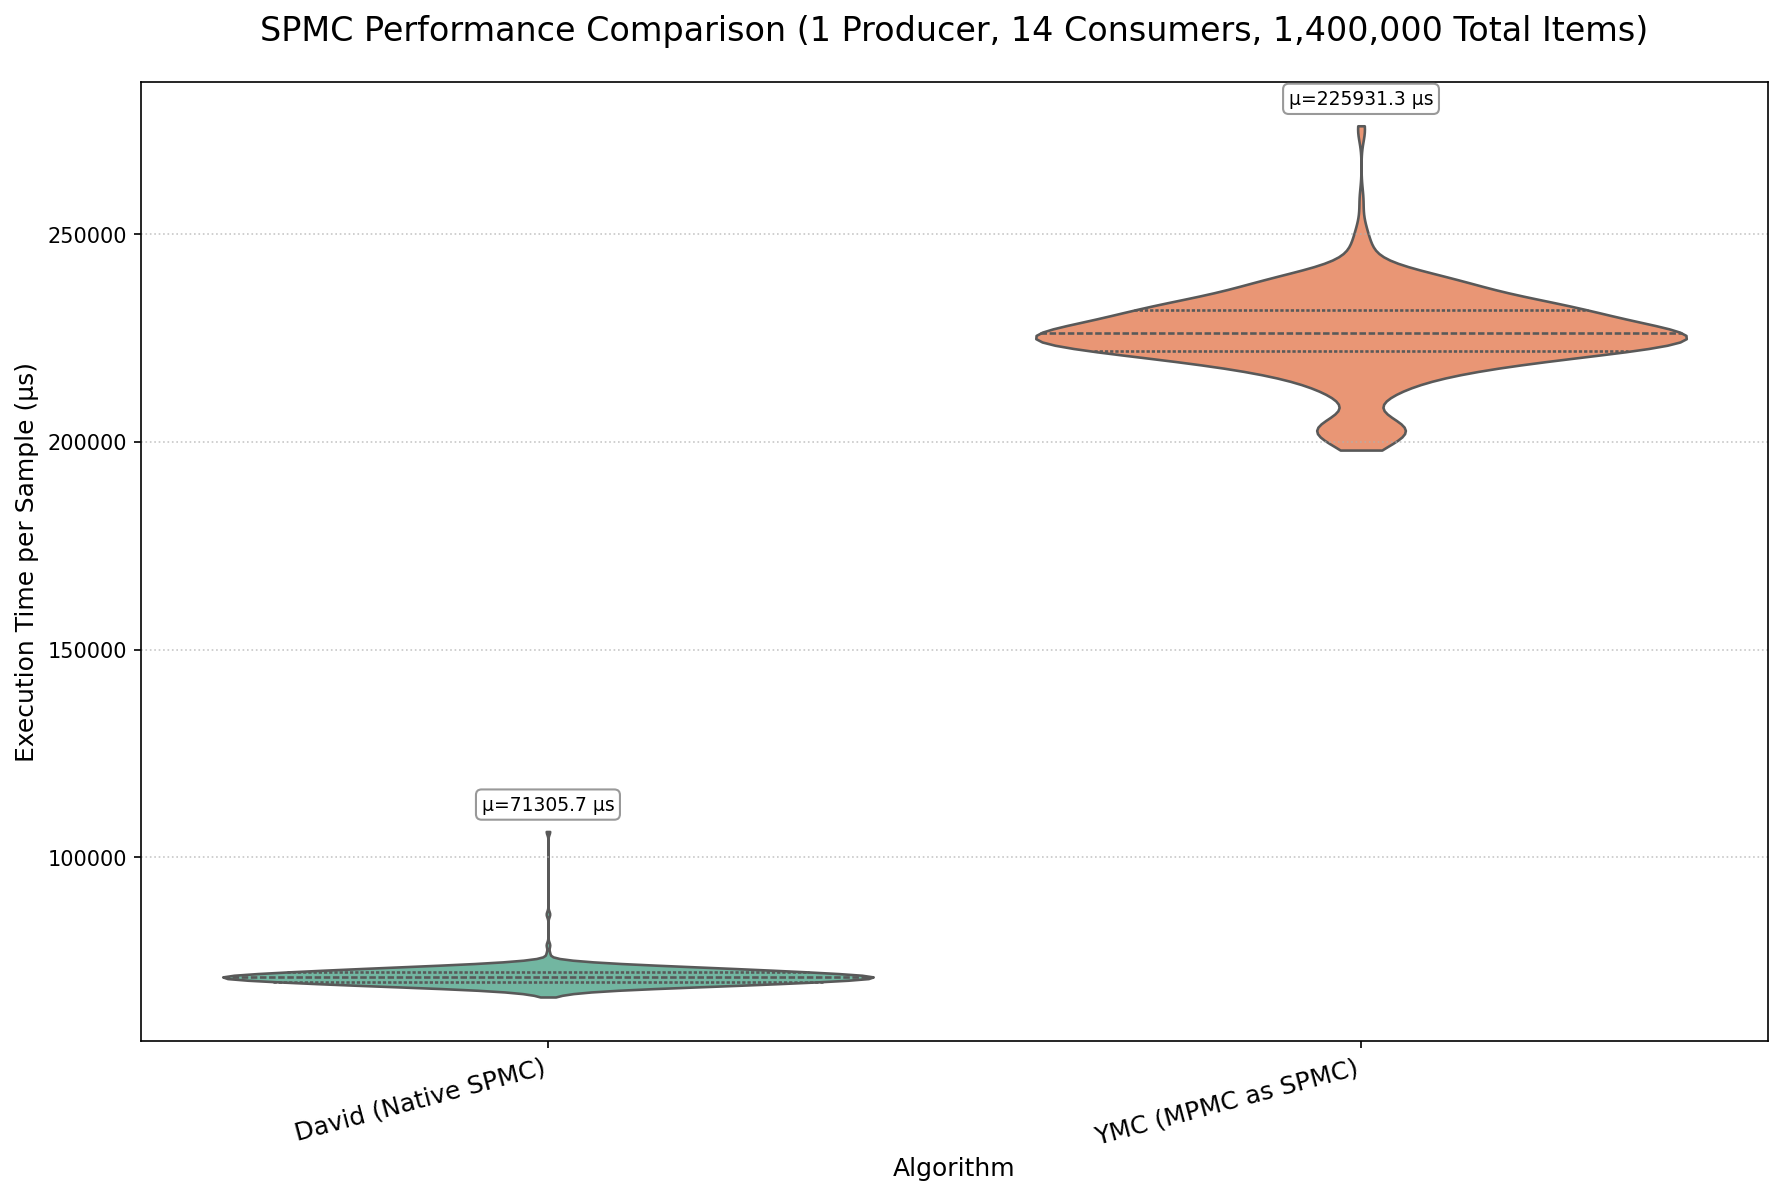
\includegraphics[width=\textwidth]{images/results/best_in_spmc_performance_violin_1P14C.png}
\end{figure}

The violin plot in \cref{fig:spmc-violin-14c} demonstrates the performance distribution under maximum consumer contention. The David queue shows more consistent performance with a tighter distribution whilst being faster compared to \ac{YMC} operating in SPMC mode, confirming again specialised queues are the better choice. Also here the same can be said for lesser consumer counts as seen in \cref{fig:cross-spmc-violin-1c,fig:cross-spmc-violin-2c,fig:cross-spmc-violin-4c,fig:cross-spmc-violin-8c}.

\begin{figure}[htb]
\centering
\caption{Mean execution time comparison of David (native SPMC) vs YMC (as SPMC) across different consumer counts}
\label{fig:cross-spmc-mean}
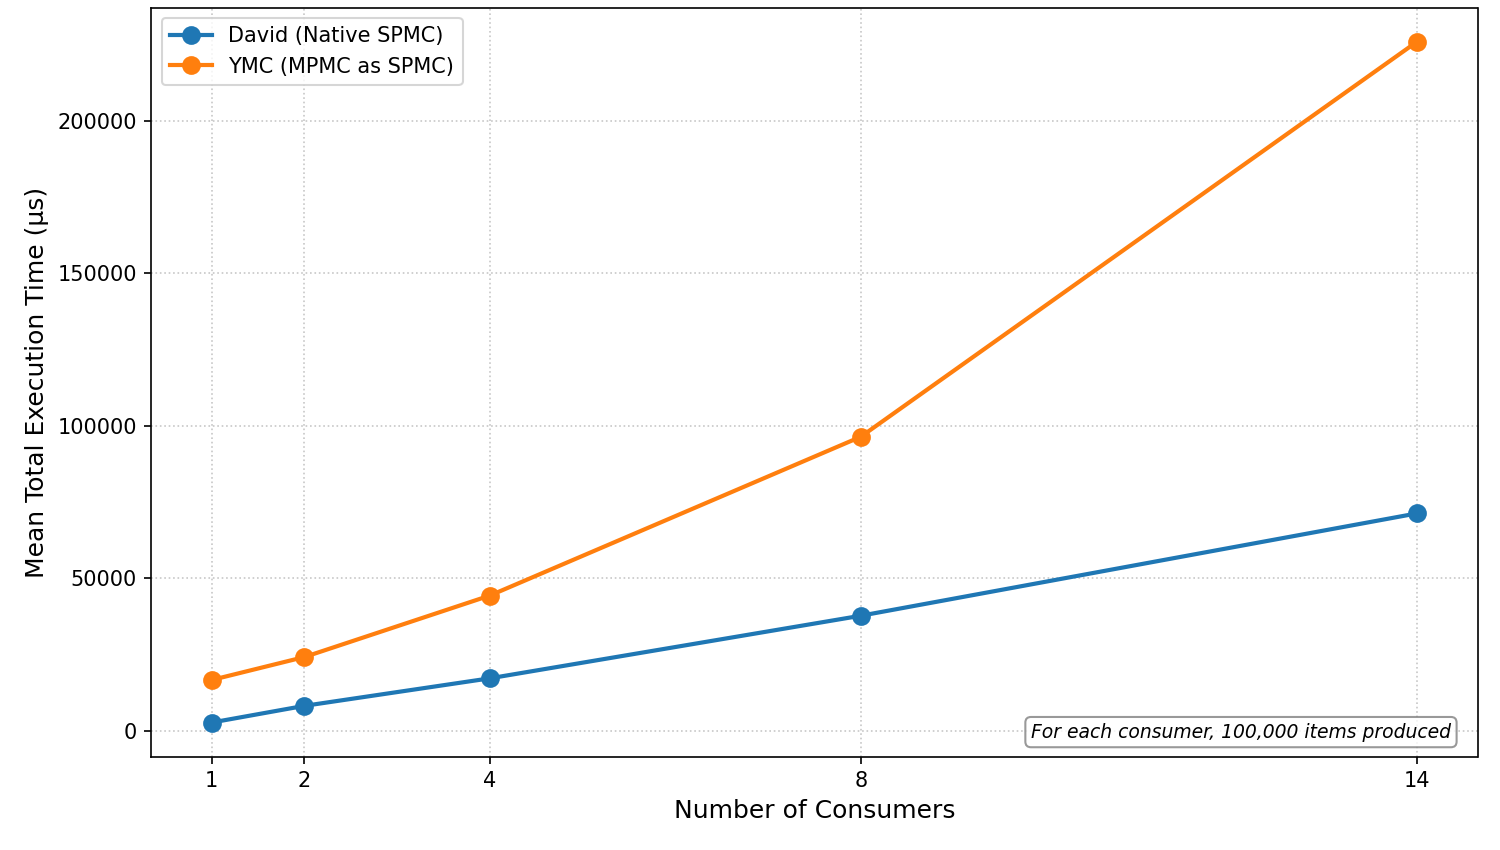
\includegraphics[width=\textwidth]{images/results/best_in_spmc_mean_performance_vs_consumers.png}
\end{figure}
    \chapter{Conclusion and Future Work}\label{ch:conclusion}

\section{Conclusion}

This thesis investigated wait-free data structures for \ac{IPC} through shared memory for \acsp{RTS}, with implementations in Rust. The primary goal was to identify and evaluate the best wait-free algorithms that can provide predictable timing guarantees essential for \ac{HRTS}.

Through systematic analysis of 20 different wait-free queue implementations across four contention categories (\ac{SPSC}, \ac{MPSC}, \ac{SPMC}, and \ac{MPMC}), several key insights emerged. First, specialization matters significantly in concurrent data structures. The benchmarks demonstrated that algorithms optimized for specific producer-consumer settings outperformes solutions build for other contention categories by factors of 2 to 10. This performance gap justifies maintaining separate implementations for different contention scenarios rather than as an example relying on a single \ac{MPMC} queue for all use cases.

Cache optimization and batching proved to be a critical factor for performance. The \acf{BLQ} achieved the best \ac{SPSC} performance at 65.2 milliseconds for 35 million items, due to its cache-aware design that minimizes false sharing by cache line seperation and batching through a producer which accumulates data before pushing them and making them visisble for a consumer. Similarly, DQueue was the best performing queue in the \ac{MPSC} category by using batching. These results confirm that understanding and optimizing cache hierarchies is important too than just proven better theoretical algorithmic time complexity like \ac{JPQ} in practice.

The implementation challenges of adapting thread-based algorithms to \ac{IPC} revealed important practical considerations. Dynamic memory allocation, which is simpler in thread-based implementations, required significant redesign for shared memory contexts. All queues using dynamic allocation had to be modified to use pre-allocated memory pools, introducing additional complexity but ensuring position-independent operation across different process address spaces. This adaptation particularly impacted the performance of \ac{dSPSC} and \ac{uSPSC} queues.

The Rust programming language was well-suited for implementing these algorithms. Its ownership model and explicit memory ordering semantics allowed precise control over synchronization while maintaining memory safety. The unsafe blocks required for shared memory operations were well-contained, and the type system helped prevent common concurrency bugs during development. The achieved test coverage of 81.12\% function coverage and 70.03\% line coverage demonstrates that most code paths could be reliably tested despite the complexity of concurrent operations. These tests with the additional correctnes check in the benchmark also formed the validation, that these queues work as expected.

Based on the comprehensive benchmarks, the recommended wait-free queues for real-time IPC are:
\begin{itemize}
\item \ac{SPSC}: \acf{BLQ}
\item \ac{MPSC}: DQueue
\item \ac{SPMC}: David Queue
\item \ac{MPMC}: Yang-Mellor-Crummey Queue for high contention scenarios, or Verma Queue when predictability is more important than raw performance
\end{itemize}

These findings contribute to \ac{RTS} by providing concrete performance data for wait-free algorithms under realistic \ac{IPC} workloads, and offering production-ready Rust implementations suitable for safety-critical applications.

\section{Future Work}
While this thesis provides a comprehensive evaluation of existing wait-free algorithms for \ac{IPC}, several areas need further research.

\subsection{Dynamic Wait-Free Memory Allocation for Shared Memory \acf{IPC}}
The most problematic area during implementation was the lack of wait-free dynamic memory allocation schemes suitable for shared memory contexts. All algorithms requiring dynamic allocation had to be modified to use pre-allocated pools, which limits flexibility and potentially wastes memory. Future research should investigate wait-free memory allocators specifically designed for shared memory \ac{IPC}.

Such allocators need to address following challenge. They must operate without a global heap, as each process has its own address space. So such an allocator would need to share the address space of the shared memory region across all processes in a wait-free manner. Also it needs to function so that dynamically the shared memory region can shrink and grow as needed while sharing the new memory region bounds to the processes while still maintaining wait-freedom.

A wait-free shared memory allocator would enable more flexible data structures and could allow the exact implementation of dynamic queues like \ac{dSPSC} and \ac{uSPSC} that currently cannot be that dynamic with a pre-allocated pool.

\subsection{Integration with \acf{RTOS}}
The current benchmarks run on a Linux system, which introduces timing variations from scheduling and interrupts. Future work should evaluate these algorithms on \ac{RTOS} like RTEMS or QNX to see the performance in a \ac{RTS} environment. This would provide insights into how these wait-free queues perform under real-time constraints and scheduling policies.

    % \chapter{Examples}

In the following some examples for the conversion in \LaTeX{} are listed. For formal requirements, please have a look at the guidelines for the preparation of student theses at the \ac{ISW}.

\section{Listings}

An introduction for list environments with \LaTeX{} can be found at \url{https://en.wikibooks.org/wiki/LaTeX/List_Structures}.

An unordered enumeration can look like this:

\begin{itemize}
    \item Fusce tincidunt consectetur nisl a pretium. Nam sed eleifend nunc. Nulla feugiat nisl ac mauris varius, eu viverra tellus condimentum. Nullam tempus dolor a elementum con-vallis. Nam sagittis, nisi non tempor luctus, enim ex pretium nunc, lacinia suscipit arcu augue id sem.
    \item Fusce tincidunt consectetur nisl a pretium. Nam sed eleifend nunc. Nulla feugiat nisl ac mauris varius, eu viverra tellus condimentum. Nullam tempus dolor a elementum con-vallis. Nam sagittis, nisi non tempor luctus, enim ex pretium nunc, lacinia suscipit arcu augue id sem.
    \item Fusce tincidunt consectetur nisl a pretium. Nam sed eleifend nunc. Nulla feugiat nisl ac mauris varius, eu viverra tellus condimentum. Nullam tempus dolor a elementum con-vallis. Nam sagittis, nisi non tempor luctus, enim ex pretium nunc, lacinia suscipit arcu augue id sem.
\end{itemize}

Use the \texttt{enumerate} environment for ordered lists.

\begin{enumerate}
    \item Fusce tincidunt consectetur nisl a pretium. Nam sed eleifend nunc. Nulla feugiat nisl ac mauris varius, eu viverra tellus condimentum. Nullam tempus dolor a elementum con-vallis. Nam sagittis, nisi non tempor luctus, enim ex pretium nunc, lacinia suscipit arcu augue id sem.
    \item Fusce tincidunt consectetur nisl a pretium. Nam sed eleifend nunc. Nulla feugiat nisl ac mauris varius, eu viverra tellus condimentum. Nullam tempus dolor a elementum con-vallis. Nam sagittis, nisi non tempor luctus, enim ex pretium nunc, lacinia suscipit arcu augue id sem.
    \item Fusce tincidunt consectetur nisl a pretium. Nam sed eleifend nunc. Nulla feugiat nisl ac mauris varius, eu viverra tellus condimentum. Nullam tempus dolor a elementum con-vallis. Nam sagittis, nisi non tempor luctus, enim ex pretium nunc, lacinia suscipit arcu augue id sem.
\end{enumerate}

Descriptions are set with the \texttt{description} environment.

\begin{description}
    \item[Mosquito] Fusce tincidunt consectetur nisl a pretium. Nam sed eleifend nunc. Nulla feugiat nisl ac mauris varius, eu viverra tellus condimentum. Nullam tempus dolor a elementum con-vallis. Nam sagittis, nisi non tempor luctus, enim ex pretium nunc, lacinia suscipit arcu augue id sem.
    \item[Emu] Fusce tincidunt consectetur nisl a pretium. Nam sed eleifend nunc. Nulla feugiat nisl ac mauris varius, eu viverra tellus condimentum. Nullam tempus dolor a elementum con-vallis. Nam sagittis, nisi non tempor luctus, enim ex pretium nunc, lacinia suscipit arcu augue id sem.
    \item[Armadillo] Fusce tincidunt consectetur nisl a pretium. Nam sed eleifend nunc. Nulla feugiat nisl ac mauris varius, eu viverra tellus condimentum. Nullam tempus dolor a elementum con-vallis. Nam sagittis, nisi non tempor luctus, enim ex pretium nunc, lacinia suscipit arcu augue id sem.
\end{description}

\section{Cite}

Cite with the \texttt{\textbackslash cite\{\}} command \cite{Cochran2005,Cubitt2013}.
You can mention authors and titles as well with \texttt{\textbackslash citeauthor\{\}} and \texttt{\textbackslash citetitle\{\}}: E.g., \citeauthor{Feuersaenger2014} developed \texttt{pgfplots} and describes it in the documentation \textit{\citetitle{Feuersaenger2014}}.

Use tools for literature management as JabRef or Citavi.

\section{Typing math}

An introduction for typing math with \LaTeX{} can be found at \url{https://de.wikibooks.org/wiki/LaTeX-Kompendium:_F%C3%BCr_Mathematiker}.
The Wikipedia page for typesetting math is worth a visit as well (\url{https://de.wikipedia.org/wiki/Formelsatz}).

You can use \texttt{\textbackslash( \ldots \textbackslash)} to typeset fomulas in text e.g., \(\sqrt{\alpha^2}\)) or \( \bmat{a & b & c}^\T \) (\texttt{\textbackslash bmat} and \texttt{\textbackslash T} are self-defined macros from \texttt{settings.tex}).

Multiline math environments can e.g. be set with the \texttt{align} environment. A \& character helps with the vertical alignment.

\begin{align}
c^2 &= a^2 + b^2 \nonumber \\
\Leftrightarrow \quad c &= \pm \sqrt{a^2 + b^2} \label{eq:pythagoras_solution}
\end{align}


Only number equations that will be referenced later, such as \autoref{eq:pythagoras_solution}. 
\texttt{\textbackslash nonumber} suppresses the generation of an equation number.

\section{Tables}

Tasbles are set in a \texttt{table} environment, as shown in \autoref{tab:animalPrices}.
They must always be referenced and explained in the previous text.
The package \href{https://ctan.kako-dev.de/macros/latex/contrib/booktabs/booktabs.pdf}{\texttt{booktabs}} faciliates the consistent use of horizontal line strenghts.

    \begin{table}[htb]
    \centering
    \begin{tabular}{@{}llr@{}} \toprule
    \multicolumn{2}{c}{Article}             \\ \cmidrule(r){1-2}
        Animal   & Description  & Price (€) \\ \midrule
        Mosquito & per gramm    & 13.65     \\
                 & per piece    & 0.01      \\
        Gnu      & stuffed      & 92.50     \\
        Emu      & stuffed      & 33.33     \\
        Armadillo& frozen       & 8.99      \\ \bottomrule
    \end{tabular}
    \caption{Example table using the booktabs package} 
    \label{tab:animalPrices}
    \end{table}

\section{Graphics}

Simple graphics can be integrated with \texttt{\textbackslash includegraphics}. Always use a \texttt{figure} environment for graphics. Reference graphics before they appear in the text, such as \autoref{fig:ustutt_logo}, and assign meaningful captions to them.

\begin{figure}[htb]
\centering

\includegraphics[width=0.5\textwidth]{images/logo-isw-uni-de.eps}
\caption{The logo of the \ac{ISW} at the University of Stuttgart}
\label{fig:ustutt_logo}
\end{figure}

Some graphics with TikZ and PGFplots are shown on \autoref{fig:blockDiagram}, \autoref{fig:timeseries_states}, \autoref{fig:timeseries_input} and \autoref{fig:phasenplot} which might be helpful or inspirational for your thesis.


\begin{figure}[htbp]
    \centering
    \begin{tikzpicture}

    \node[block] (controller) {Controller\\ \(k(e)\)};
    \node[block, right=2cm of controller] (plant) {Plant\\ \(\dot x = f(x,u) \)\\ \(y=h(x) \)};

    \node[sum, left = of controller] (err) {};

    \draw[->] (controller) -- node[above]{\(u\)} (plant);
    \draw[->] (err) -- node[above]{\(e\)}(controller);

    \draw[->](plant) -- node[above]{\(y\)} ++(2cm, 0);
    \draw[->] (plant) -| ++(1.5cm,-1.2cm) -| node[right, pos=0.95]{\(-\)} (err);

    \draw[<-] (err) -- node[left, pos=1]{\(y_\mathrm{des}\)} ++(-2cm, 0);

\end{tikzpicture}
    \caption{A simple block diagram}
    \label{fig:blockDiagram}
\end{figure}

\begin{figure}[htbp]

\centering
\begin{subfigure}[b]{0.95\textwidth}
    % This file was created by matlab2tikz.
%
\definecolor{mycolor1}{rgb}{0.00000,0.56863,0.86275}%
\definecolor{mycolor2}{rgb}{1.00000,0.54902,0.14902}%
\definecolor{mycolor3}{rgb}{0.30588,0.74118,0.35294}%
%
\begin{tikzpicture}

\begin{axis}[%
width=0.951\figurewidth,
height=\figureheight,
at={(0\figurewidth,0\figureheight)},
scale only axis,
xmin=0,
xmax=5,
xlabel={Time \(t\) [s]},
y label style={at={(-0.112,0.5)}},
ymin=-10,
ymax=10,
ylabel={States},
axis background/.style={fill=white},
axis x line*=bottom,
axis y line*=left,
legend style={legend cell align=left,align=left,draw=white!15!black, at={(axis description cs:.89,1.3)},anchor=north}
]
\addplot [color=mycolor1,solid]
  table[row sep=crcr]{%
0	5\\
0.01	4.99524563586321\\
0.02	4.98101630642928\\
0.03	4.95737192324524\\
0.04	4.92438893489464\\
0.05	4.88216801700883\\
0.06	4.83084726513787\\
0.07	4.77062670520508\\
0.08	4.70181889185563\\
0.09	4.62496936786054\\
0.1	4.54120118871523\\
0.11	4.45324665779081\\
0.12	4.36455130558219\\
0.13	4.27708125431517\\
0.14	4.19134969607215\\
0.15	4.10733805689558\\
0.16	4.0250141878598\\
0.17	3.94434437737414\\
0.18	3.86529525509785\\
0.19	3.78783408212801\\
0.2	3.71192878308595\\
0.21	3.63754793864312\\
0.22	3.56466077249035\\
0.23	3.49323713780655\\
0.24	3.42324750393716\\
0.25	3.35466294336984\\
0.26	3.28745511901083\\
0.27	3.22159627175465\\
0.28	3.1570592083387\\
0.29	3.0938172894748\\
0.3	3.03184441824977\\
0.31	2.97111502878778\\
0.32	2.91160407516711\\
0.33	2.85328702058463\\
0.34	2.79613982676135\\
0.35	2.74013894358264\\
0.36	2.6852612989671\\
0.37	2.63148428895808\\
0.38	2.57878576803231\\
0.39	2.52714403962003\\
0.4	2.47653784683139\\
0.41	2.42694636338398\\
0.42	2.37834918472657\\
0.43	2.33072631935423\\
0.44	2.28405818031023\\
0.45	2.23832557687022\\
0.46	2.19350970640432\\
0.47	2.14959214641296\\
0.48	2.10655484673226\\
0.49	2.06438012190512\\
0.5	2.02305064371406\\
0.51	1.98254943387211\\
0.52	1.94285985686812\\
0.53	1.90396561296289\\
0.54	1.86585073133274\\
0.55	1.8284995633572\\
0.56	1.79189677604749\\
0.57	1.75602734561261\\
0.58	1.72087655116011\\
0.59	1.68642996852835\\
0.6	1.65267346424742\\
0.61	1.6195931896259\\
0.62	1.58717557496055\\
0.63	1.55540732386645\\
0.64	1.52427540772469\\
0.65	1.49376706024524\\
0.66	1.46386977214239\\
0.67	1.43457128592035\\
0.68	1.4058595907666\\
0.69	1.3777229175507\\
0.7	1.35014973392623\\
0.71	1.32312873953367\\
0.72	1.29664886130212\\
0.73	1.27069924884756\\
0.74	1.24526926996584\\
0.75	1.22034850621815\\
0.76	1.19592674860714\\
0.77	1.17199399334169\\
0.78	1.14854043768858\\
0.79	1.12555647590896\\
0.8	1.10303269527819\\
0.81	1.0809598721869\\
0.82	1.05932896832193\\
0.83	1.03813112692517\\
0.84	1.01735766912884\\
0.85	0.997000090365587\\
0.86	0.977050056851735\\
0.87	0.957499402142291\\
0.88	0.938340123756105\\
0.89	0.919564379869777\\
0.9	0.901164486078865\\
0.91	0.883132912224982\\
0.92	0.865462279287434\\
0.93	0.848145356338032\\
0.94	0.831175057557802\\
0.95	0.814544439314279\\
0.96	0.798246697298145\\
0.97	0.782275163717989\\
0.98	0.766623304551978\\
0.99	0.751284716855268\\
1	0.736253126122008\\
1.01	0.72152238370081\\
1.02	0.707086464262578\\
1.03	0.692939463319636\\
1.04	0.679075594795081\\
1.05	0.665489188641335\\
1.06	0.6521746885069\\
1.07	0.639126649450301\\
1.08	0.626339735700277\\
1.09	0.613808718461249\\
1.1	0.601528473763155\\
1.11	0.589493980354737\\
1.12	0.577700317639388\\
1.13	0.566142663652695\\
1.14	0.554816293080827\\
1.15	0.543716575318924\\
1.16	0.53283897256869\\
1.17	0.52217903797436\\
1.18	0.5117324137963\\
1.19	0.501494829621425\\
1.2	0.491462100609733\\
1.21	0.481630125776181\\
1.22	0.471994886307207\\
1.23	0.462552443911186\\
1.24	0.453298939202125\\
1.25	0.444230590115933\\
1.26	0.435343690358591\\
1.27	0.42663460788559\\
1.28	0.41809978341198\\
1.29	0.409735728952434\\
1.3	0.401539026390699\\
1.31	0.393506326077847\\
1.32	0.385634345458741\\
1.33	0.377919867726138\\
1.34	0.370359740501881\\
1.35	0.362950874544623\\
1.36	0.355690242483541\\
1.37	0.348574877577528\\
1.38	0.341601872499339\\
1.39	0.334768378144179\\
1.4	0.328071602462255\\
1.41	0.321508809314795\\
1.42	0.315077317353064\\
1.43	0.308774498919909\\
1.44	0.302597778973388\\
1.45	0.296544634032018\\
1.46	0.290612591141226\\
1.47	0.284799226860563\\
1.48	0.27910216627126\\
1.49	0.273519082003727\\
1.5	0.268047693284576\\
1.51	0.262685765002797\\
1.52	0.257431106794671\\
1.53	0.252281572147071\\
1.54	0.247235057518759\\
1.55	0.242289501479331\\
1.56	0.237442883865443\\
1.57	0.232693224953979\\
1.58	0.228038584651809\\
1.59	0.223477061701814\\
1.6	0.219006792904847\\
1.61	0.2146259523573\\
1.62	0.210332750703979\\
1.63	0.20612543440596\\
1.64	0.202002285023145\\
1.65	0.197961618511203\\
1.66	0.19400178453262\\
1.67	0.190121165781565\\
1.68	0.186318177322301\\
1.69	0.182591265940867\\
1.7	0.178938909509756\\
1.71	0.175359616365342\\
1.72	0.171851924697786\\
1.73	0.168414401953182\\
1.74	0.165045644247681\\
1.75	0.161744275793374\\
1.76	0.158508948335677\\
1.77	0.155338340601997\\
1.78	0.152231157761455\\
1.79	0.149186130895436\\
1.8	0.14620201647875\\
1.81	0.143277595871199\\
1.82	0.140411674819329\\
1.83	0.137603082968172\\
1.84	0.13485067338277\\
1.85	0.132153322079294\\
1.86	0.129509927565553\\
1.87	0.126919410390713\\
1.88	0.124380712704042\\
1.89	0.121892797822495\\
1.9	0.119454649806958\\
1.91	0.117065273046993\\
1.92	0.114723691853893\\
1.93	0.112428950061896\\
1.94	0.110180110637387\\
1.95	0.107976255295926\\
1.96	0.105816484126954\\
1.97	0.103699915226012\\
1.98	0.101625684334327\\
1.99	0.0995929444856207\\
2	0.0976008656599932\\
2.01	0.0956486344447337\\
2.02	0.0937354537019301\\
2.03	0.0918605422427345\\
2.04	0.0900231345081515\\
2.05	0.0882224802562205\\
2.06	0.0864578442554627\\
2.07	0.0847285059844664\\
2.08	0.0830337593374898\\
2.09	0.0813729123359575\\
2.1	0.0797452868457358\\
2.11	0.0781502183000684\\
2.12	0.0765870554280602\\
2.13	0.0750551599885981\\
2.14	0.0735539065095992\\
2.15	0.0720826820324799\\
2.16	0.0706408858617417\\
2.17	0.0692279293195698\\
2.18	0.0678432355053461\\
2.19	0.0664862390599761\\
2.2	0.0651563859349345\\
2.21	0.063853133165934\\
2.22	0.0625759486511263\\
2.23	0.0613243109337417\\
2.24	0.0600977089890819\\
2.25	0.0588956420157753\\
2.26	0.0577176192312117\\
2.27	0.0565631596710725\\
2.28	0.0554317919928724\\
2.29	0.0543230542834351\\
2.3	0.0532364938702222\\
2.31	0.0521716671364379\\
2.32	0.051128139339836\\
2.33	0.0501054844351527\\
2.34	0.0491032849000937\\
2.35	0.0481211315648043\\
2.36	0.047158623444753\\
2.37	0.0462153675769591\\
2.38	0.0452909788594991\\
2.39	0.0443850798942244\\
2.4	0.0434973008326277\\
2.41	0.0426272792247931\\
2.42	0.0417746598713706\\
2.43	0.0409390946785115\\
2.44	0.0401202425157088\\
2.45	0.0393177690764809\\
2.46	0.0385313467418442\\
2.47	0.0377606544465182\\
2.48	0.0370053775478075\\
2.49	0.036265207697108\\
2.5	0.0355398427139845\\
2.51	0.0348289864627682\\
2.52	0.0341323487316235\\
2.53	0.0334496451140347\\
2.54	0.0327805968926651\\
2.55	0.0321249309255386\\
2.56	0.0314823795345005\\
2.57	0.0308526803959092\\
2.58	0.0302355764335155\\
2.59	0.0296308157134852\\
2.6	0.0290381513415229\\
2.61	0.0284573413620531\\
2.62	0.0278881486594202\\
2.63	0.0273303408610638\\
2.64	0.0267836902426327\\
2.65	0.0262479736349967\\
2.66	0.0257229723331194\\
2.67	0.0252084720067538\\
2.68	0.0247042626129254\\
2.69	0.0242101383101659\\
2.7	0.0237258973744633\\
2.71	0.0232513421168933\\
2.72	0.0227862788028987\\
2.73	0.0223305175731846\\
2.74	0.0218838723661952\\
2.75	0.0214461608421425\\
2.76	0.0210172043085545\\
2.77	0.0205968276473135\\
2.78	0.0201848592431533\\
2.79	0.0197811309135881\\
2.8	0.0193854778402421\\
2.81	0.018997738501554\\
2.82	0.0186177546068275\\
2.83	0.0182453710316005\\
2.84	0.0178804357543089\\
2.85	0.0175227997942161\\
2.86	0.0171723171505848\\
2.87	0.0168288447430663\\
2.88	0.0164922423532811\\
2.89	0.0161623725675697\\
2.9	0.0158391007208875\\
2.91	0.0155222948418231\\
2.92	0.0152118255987158\\
2.93	0.0149075662468514\\
2.94	0.0146093925767144\\
2.95	0.0143171828632754\\
2.96	0.0140308178162931\\
2.97	0.0137501805316101\\
2.98	0.0134751564434236\\
2.99	0.0132056332775109\\
3	0.01294150100539\\
3.01	0.0126826517993978\\
3.02	0.0124289799886672\\
3.03	0.0121803820159839\\
3.04	0.011936756395507\\
3.05	0.0116980036713357\\
3.06	0.0114640263769038\\
3.07	0.0112347289951873\\
3.08	0.0110100179197082\\
3.09	0.0107898014163173\\
3.1	0.0105739895857429\\
3.11	0.0103624943268876\\
3.12	0.01015522930086\\
3.13	0.00995210989572565\\
3.14	0.00975305319196289\\
3.15	0.00955797792861027\\
3.16	0.00936680447009072\\
3.17	0.00917945477369952\\
3.18	0.00899585235774264\\
3.19	0.00881592227031242\\
3.2	0.00863959105868787\\
3.21	0.00846678673934707\\
3.22	0.00829743876857945\\
3.23	0.00813147801368588\\
3.24	0.00796883672475497\\
3.25	0.00780944850700381\\
3.26	0.00765324829367213\\
3.27	0.00750017231945856\\
3.28	0.00735015809448833\\
3.29	0.00720314437880167\\
3.3	0.00705907115735255\\
3.31	0.0069178796155075\\
3.32	0.00677951211503458\\
3.33	0.00664391217057259\\
3.34	0.00651102442657104\\
3.35	0.00638079463469133\\
3.36	0.00625316963166003\\
3.37	0.00612809731756512\\
3.38	0.00600552663458642\\
3.39	0.00588540754615141\\
3.4	0.00576769101650809\\
3.41	0.00565232899070635\\
3.42	0.00553927437497982\\
3.43	0.00542848101752017\\
3.44	0.00531990368963586\\
3.45	0.00521349806728796\\
3.46	0.00510922071299512\\
3.47	0.00500702905810059\\
3.48	0.00490688138539393\\
3.49	0.00480873681208035\\
3.5	0.00471255527309068\\
3.51	0.00461829750472517\\
3.52	0.00452592502862454\\
3.53	0.00443540013606154\\
3.54	0.00434668587254682\\
3.55	0.00425974602274267\\
3.56	0.00417454509567851\\
3.57	0.00409104831026216\\
3.58	0.00400922158108088\\
3.59	0.00392903150448643\\
3.6	0.00385044534495849\\
3.61	0.00377343102174081\\
3.62	0.00369795709574468\\
3.63	0.00362399275671439\\
3.64	0.00355150781064938\\
3.65	0.00348047266747795\\
3.66	0.00341085832897762\\
3.67	0.00334263637693702\\
3.68	0.0032757789615546\\
3.69	0.00321025879006939\\
3.7	0.0031460491156192\\
3.71	0.00308312372632161\\
3.72	0.00302145693457347\\
3.73	0.0029610235665643\\
3.74	0.0029017989519996\\
3.75	0.00284375891402958\\
3.76	0.00278687975937939\\
3.77	0.00273113826867681\\
3.78	0.00267651168697333\\
3.79	0.00262297771445489\\
3.8	0.00257051449733836\\
3.81	0.00251910061895021\\
3.82	0.0024687150909835\\
3.83	0.00241933734492987\\
3.84	0.00237094722368279\\
3.85	0.00232352497330888\\
3.86	0.00227705123498373\\
3.87	0.00223150703708906\\
3.88	0.00218687378746794\\
3.89	0.00214313326583494\\
3.9	0.00210026761633806\\
3.91	0.00205825934026946\\
3.92	0.00201709128892201\\
3.93	0.00197674665658865\\
3.94	0.00193720897370186\\
3.95	0.00189846210011028\\
3.96	0.0018604902184899\\
3.97	0.00182327782788695\\
3.98	0.00178680973738996\\
3.99	0.00175107105992847\\
4	0.00171604720619566\\
4.01	0.00168172387869265\\
4.02	0.00164808706589181\\
4.03	0.00161512303651694\\
4.04	0.00158281833393774\\
4.05	0.0015511597706765\\
4.06	0.00152013442302458\\
4.07	0.00148972962576663\\
4.08	0.00145993296701033\\
4.09	0.0014307322831195\\
4.1	0.0014021156537486\\
4.11	0.00137407139697654\\
4.12	0.00134658806453781\\
4.13	0.00131965443714901\\
4.14	0.00129325951992883\\
4.15	0.00126739253790971\\
4.16	0.00124204293163917\\
4.17	0.0012172003528692\\
4.18	0.00119285466033184\\
4.19	0.00116899591559926\\
4.2	0.00114561437902665\\
4.21	0.00112270050577624\\
4.22	0.0011002449419209\\
4.23	0.00107823852062557\\
4.24	0.00105667225840521\\
4.25	0.00103553735145744\\
4.26	0.0010148251720687\\
4.27	0.000994527265092134\\
4.28	0.000974635344496026\\
4.29	0.000955141289981249\\
4.3	0.000936037143666347\\
4.31	0.000917315106838946\\
4.32	0.000898967536772131\\
4.33	0.000880986943604504\\
4.34	0.000863365987282643\\
4.35	0.00084609747456472\\
4.36	0.000829174356084049\\
4.37	0.000812589723471371\\
4.38	0.000796336806534692\\
4.39	0.000780408970495536\\
4.4	0.000764799713280473\\
4.41	0.00074950266286682\\
4.42	0.000734511574681436\\
4.43	0.00071982032905154\\
4.44	0.000705422928706523\\
4.45	0.000691313496329723\\
4.46	0.000677486272159168\\
4.47	0.000663935611636311\\
4.48	0.000650655983101793\\
4.49	0.000637641965537295\\
4.5	0.00062488824635255\\
4.51	0.000612389619216631\\
4.52	0.000600140981932601\\
4.53	0.00058813733435469\\
4.54	0.000576373776347115\\
4.55	0.000564845505783741\\
4.56	0.000553547816587741\\
4.57	0.000542476096810475\\
4.58	0.000531625826748785\\
4.59	0.000520992577099955\\
4.6	0.000510572007153569\\
4.61	0.000500359863019541\\
4.62	0.000490351975891579\\
4.63	0.000480544260345386\\
4.64	0.000470932712670905\\
4.65	0.00046151340923791\\
4.66	0.000452282504894298\\
4.67	0.000443236231396416\\
4.68	0.000434370895870775\\
4.69	0.000425682879306543\\
4.7	0.000417168635078186\\
4.71	0.000408824687497658\\
4.72	0.000400647630395548\\
4.73	0.000392634125730609\\
4.74	0.000384780902227098\\
4.75	0.000377084754039369\\
4.76	0.000369542539443182\\
4.77	0.000362151179553175\\
4.78	0.000354907657066006\\
4.79	0.00034780901502862\\
4.8	0.000340852355631157\\
4.81	0.000334034839024008\\
4.82	0.000327353682158522\\
4.83	0.000320806157650911\\
4.84	0.000314389592668871\\
4.85	0.000308101367840477\\
4.86	0.000301938916184898\\
4.87	0.0002958997220645\\
4.88	0.000289981320157913\\
4.89	0.000284181294453631\\
4.9	0.000278497277263747\\
4.91	0.000272926948257411\\
4.92	0.000267468033513624\\
4.93	0.000262118304592973\\
4.94	0.00025687557762794\\
4.95	0.000251737712431393\\
4.96	0.000246702611622926\\
4.97	0.000241768219772656\\
4.98	0.00023693252256216\\
4.99	0.000232193545962184\\
5	0.000227549355426803\\
};
\addlegendentry{\(x_1\)};

\addplot [color=mycolor2,solid]
  table[row sep=crcr]{%
0	0\\
0.01	-0.950069425216098\\
0.02	-1.89479883271611\\
0.03	-2.83280850295291\\
0.04	-3.76212444792955\\
0.05	-4.67978948168419\\
0.06	-5.58110481588912\\
0.07	-6.4580023585369\\
0.08	-7.2950933736677\\
0.09	-8.05850219503889\\
0.1	-8.66077297554567\\
0.11	-8.92697884398766\\
0.12	-8.83472707109159\\
0.13	-8.660262815696\\
0.14	-8.4866931759622\\
0.15	-8.31621529806666\\
0.16	-8.14911906466565\\
0.17	-7.98539087296735\\
0.18	-7.8249700780463\\
0.19	-7.66779007263986\\
0.2	-7.51378460697885\\
0.21	-7.36288869414473\\
0.22	-7.2150387091042\\
0.23	-7.07017237391279\\
0.24	-6.92822872835011\\
0.25	-6.78914809950282\\
0.26	-6.65287207201148\\
0.27	-6.5193434591569\\
0.28	-6.38850627477295\\
0.29	-6.26030570595285\\
0.3	-6.13468808651583\\
0.31	-6.01160087120313\\
0.32	-5.89099261057402\\
0.33	-5.77281292657441\\
0.34	-5.65701248875245\\
0.35	-5.54354299109672\\
0.36	-5.4323571294743\\
0.37	-5.32340857964711\\
0.38	-5.21665197584623\\
0.39	-5.11204288988477\\
0.4	-5.00953781079131\\
0.41	-4.90909412494632\\
0.42	-4.81067009670531\\
0.43	-4.71422484949296\\
0.44	-4.6197183473534\\
0.45	-4.52711137694247\\
0.46	-4.43636552994837\\
0.47	-4.34744318592778\\
0.48	-4.26030749554524\\
0.49	-4.17492236420371\\
0.5	-4.09125243605526\\
0.51	-4.00926307838084\\
0.52	-3.92892036632888\\
0.53	-3.85019106800254\\
0.54	-3.77304262988624\\
0.55	-3.69744316260205\\
0.56	-3.62336142698709\\
0.57	-3.55076682048353\\
0.58	-3.47962936383268\\
0.59	-3.40991968806548\\
0.6	-3.34160902178159\\
0.61	-3.27466917870966\\
0.62	-3.20907254554167\\
0.63	-3.14479207003448\\
0.64	-3.08180124937176\\
0.65	-3.02007411877993\\
0.66	-2.95958524039193\\
0.67	-2.9003096923525\\
0.68	-2.84222305815939\\
0.69	-2.78530141623461\\
0.7	-2.72952132972031\\
0.71	-2.67485983649377\\
0.72	-2.62129443939657\\
0.73	-2.56880309667264\\
0.74	-2.51736421261042\\
0.75	-2.46695662838433\\
0.76	-2.41755961309096\\
0.77	-2.36915285497542\\
0.78	-2.32171645284355\\
0.79	-2.27523090765572\\
0.8	-2.22967711429795\\
0.81	-2.18503635352664\\
0.82	-2.14129028408257\\
0.83	-2.09842093497076\\
0.84	-2.05641069790218\\
0.85	-2.01524231989381\\
0.86	-1.97489889602357\\
0.87	-1.93536386233658\\
0.88	-1.89662098889944\\
0.89	-1.85865437299932\\
0.9	-1.82144843248458\\
0.91	-1.78498789924389\\
0.92	-1.74925781282079\\
0.93	-1.71424351416078\\
0.94	-1.6799306394879\\
0.95	-1.64630511430831\\
0.96	-1.61335314753771\\
0.97	-1.58106122575029\\
0.98	-1.54941610754638\\
0.99	-1.51840481803629\\
1	-1.48801464343792\\
1.01	-1.45823312578559\\
1.02	-1.4290480577478\\
1.03	-1.40044747755161\\
1.04	-1.3724196640112\\
1.05	-1.34495313165871\\
1.06	-1.31803662597484\\
1.07	-1.29165911871736\\
1.08	-1.26580980334531\\
1.09	-1.24047809053695\\
1.1	-1.21565360379948\\
1.11	-1.19132617516848\\
1.12	-1.16748584099538\\
1.13	-1.14412283782097\\
1.14	-1.12122759833316\\
1.15	-1.09879074740729\\
1.16	-1.07680309822717\\
1.17	-1.05525564848534\\
1.18	-1.0341395766606\\
1.19	-1.01344623837153\\
1.2	-0.99316716280415\\
1.21	-0.973294049212399\\
1.22	-0.953818763489712\\
1.23	-0.934733334810378\\
1.24	-0.916029952339164\\
1.25	-0.897700962007788\\
1.26	-0.879738863356886\\
1.27	-0.862136306442093\\
1.28	-0.84488608880293\\
1.29	-0.827981152493186\\
1.3	-0.811414581171546\\
1.31	-0.795179597251203\\
1.32	-0.77926955910725\\
1.33	-0.763677958340661\\
1.34	-0.748398417097702\\
1.35	-0.733424685443618\\
1.36	-0.718750638789502\\
1.37	-0.704370275371239\\
1.38	-0.690277713779458\\
1.39	-0.676467190539458\\
1.4	-0.66293305774007\\
1.41	-0.649669780710463\\
1.42	-0.636671935743907\\
1.43	-0.623934207867538\\
1.44	-0.611451388657181\\
1.45	-0.599218374096307\\
1.46	-0.587230162478232\\
1.47	-0.575481852350674\\
1.48	-0.563968640501786\\
1.49	-0.552685819986854\\
1.5	-0.541628778194793\\
1.51	-0.530792994953664\\
1.52	-0.520174040674383\\
1.53	-0.509767574531886\\
1.54	-0.499569342682945\\
1.55	-0.489575176519923\\
1.56	-0.47978099095972\\
1.57	-0.470182782767199\\
1.58	-0.46077662891239\\
1.59	-0.451558684960793\\
1.6	-0.442525183496099\\
1.61	-0.433672432574674\\
1.62	-0.424996814211168\\
1.63	-0.416494782894606\\
1.64	-0.408162864134358\\
1.65	-0.39999765303536\\
1.66	-0.391995812902025\\
1.67	-0.384154073870232\\
1.68	-0.376469231566842\\
1.69	-0.368938145796181\\
1.7	-0.361557739252937\\
1.71	-0.354324996260952\\
1.72	-0.347236961537366\\
1.73	-0.340290738981614\\
1.74	-0.333483490488768\\
1.75	-0.326812434786736\\
1.76	-0.320274846296827\\
1.77	-0.313868054017224\\
1.78	-0.307589440428888\\
1.79	-0.301436440423447\\
1.8	-0.29540654025263\\
1.81	-0.289497276498803\\
1.82	-0.283706235066181\\
1.83	-0.278031050192312\\
1.84	-0.272469403479405\\
1.85	-0.267019022945118\\
1.86	-0.2616776820924\\
1.87	-0.256443198998017\\
1.88	-0.251313435419374\\
1.89	-0.246286295919266\\
1.9	-0.241359727008204\\
1.91	-0.236531716303954\\
1.92	-0.231800291707942\\
1.93	-0.227163520598195\\
1.94	-0.222619509038471\\
1.95	-0.218166401003267\\
1.96	-0.213802377618367\\
1.97	-0.209525656416639\\
1.98	-0.205334490608753\\
1.99	-0.201227168368539\\
2	-0.197202012132669\\
2.01	-0.193257377914398\\
2.02	-0.189391654631065\\
2.03	-0.185603263445078\\
2.04	-0.181890657118125\\
2.05	-0.178252319378324\\
2.06	-0.174686764300076\\
2.07	-0.171192535696346\\
2.08	-0.167768206523128\\
2.09	-0.164412378295856\\
2.1	-0.161123680517511\\
2.11	-0.157900770118195\\
2.12	-0.154742330905941\\
2.13	-0.151647073028529\\
2.14	-0.148613732446092\\
2.15	-0.145641070414293\\
2.16	-0.142727872977862\\
2.17	-0.13987295047428\\
2.18	-0.137075137047415\\
2.19	-0.134333290170901\\
2.2	-0.13164629018107\\
2.21	-0.129013039819245\\
2.22	-0.1264324637832\\
2.23	-0.123903508287616\\
2.24	-0.121425140633337\\
2.25	-0.118996348785254\\
2.26	-0.116616140958661\\
2.27	-0.114283545213876\\
2.28	-0.111997609059006\\
2.29	-0.109757399060653\\
2.3	-0.107562000462427\\
2.31	-0.105410516811099\\
2.32	-0.103302069590243\\
2.33	-0.101235797861215\\
2.34	-0.0992108579113263\\
2.35	-0.0972264229090591\\
2.36	-0.0952816825661931\\
2.37	-0.0933758428066956\\
2.38	-0.0915081254422438\\
2.39	-0.0896777678542466\\
2.4	-0.0878840226822329\\
2.41	-0.0861261575184816\\
2.42	-0.0844034546087664\\
2.43	-0.0827152105590932\\
2.44	-0.0810607360483105\\
2.45	-0.0794393555464737\\
2.46	-0.0778504070388497\\
2.47	-0.0762932417554475\\
2.48	-0.0747672239059646\\
2.49	-0.0732717304200399\\
2.5	-0.0718061506927082\\
2.51	-0.0703698863349501\\
2.52	-0.0689623509292372\\
2.53	-0.0675829697899706\\
2.54	-0.0662311797287161\\
2.55	-0.0649064288241394\\
2.56	-0.0636081761965467\\
2.57	-0.0623358917869394\\
2.58	-0.0610890561404914\\
2.59	-0.0598671601943613\\
2.6	-0.0586697050697517\\
2.61	-0.0574962018681318\\
2.62	-0.0563461714715384\\
2.63	-0.0552191443468749\\
2.64	-0.0541146603541268\\
2.65	-0.0530322685584174\\
2.66	-0.0519715270458241\\
2.67	-0.0509320027428819\\
2.68	-0.0499132712397003\\
2.69	-0.0489149166166191\\
2.7	-0.0479365312743351\\
2.71	-0.0469777157674281\\
2.72	-0.0460380786412192\\
2.73	-0.0451172362718933\\
2.74	-0.044214812709823\\
2.75	-0.0433304395260269\\
2.76	-0.042463755661701\\
2.77	-0.0416144072807621\\
2.78	-0.0407820476253416\\
2.79	-0.0399663368741716\\
2.8	-0.0391669420038049\\
2.81	-0.0383835366526126\\
2.82	-0.037615800987503\\
2.83	-0.0368634215733079\\
2.84	-0.0361260912447827\\
2.85	-0.0354035089811684\\
2.86	-0.0346953797832626\\
2.87	-0.034001414552952\\
2.88	-0.033321329975154\\
2.89	-0.0326548484021221\\
2.9	-0.0320016977400656\\
2.91	-0.0313616113380381\\
2.92	-0.0307343278790499\\
2.93	-0.0301195912733586\\
2.94	-0.0295171505538952\\
2.95	-0.0289267597737829\\
2.96	-0.0283481779059063\\
2.97	-0.0277811687444898\\
2.98	-0.0272255008086461\\
2.99	-0.0266809472478538\\
3	-0.026147285749327\\
3.01	-0.0256242984472379\\
3.02	-0.0251117718337554\\
3.03	-0.0246094966718646\\
3.04	-0.0241172679099298\\
3.05	-0.0236348845979673\\
3.06	-0.0231621498055933\\
3.07	-0.0226988705416136\\
3.08	-0.0222448576752221\\
3.09	-0.0217999258587756\\
3.1	-0.0213638934521143\\
3.11	-0.0209365824483959\\
3.12	-0.0205178184014139\\
3.13	-0.0201074303543698\\
3.14	-0.0197052507700705\\
3.15	-0.0193111154625221\\
3.16	-0.0189248635298928\\
3.17	-0.0185463372888158\\
3.18	-0.0181753822100082\\
3.19	-0.0178118468551764\\
3.2	-0.017455582815185\\
3.21	-0.0171064446494617\\
3.22	-0.0167642898266153\\
3.23	-0.0164289786662412\\
3.24	-0.0161003742818915\\
3.25	-0.0157783425251855\\
3.26	-0.0154627519310388\\
3.27	-0.0151534736639879\\
3.28	-0.014850381465589\\
3.29	-0.0145533516028683\\
3.3	-0.0142622628178044\\
3.31	-0.0139769962778207\\
3.32	-0.013697435527269\\
3.33	-0.0134234664398825\\
3.34	-0.0131549771721813\\
3.35	-0.0128918581178089\\
3.36	-0.012634001862783\\
3.37	-0.012381303141641\\
3.38	-0.0121336587944632\\
3.39	-0.0118909677247552\\
3.4	-0.0116531308581734\\
3.41	-0.0114200511020761\\
3.42	-0.0111916333058832\\
3.43	-0.0109677842222298\\
3.44	-0.0107484124688958\\
3.45	-0.0105334284914985\\
3.46	-0.0103227445269298\\
3.47	-0.0101162745675263\\
3.48	-0.00991393432595537\\
3.49	-0.00971564120080383\\
3.5	-0.00952131424285493\\
3.51	-0.00933087412204004\\
3.52	-0.00914424309505138\\
3.53	-0.00896134497360261\\
3.54	-0.00878210509332435\\
3.55	-0.00860645028328189\\
3.56	-0.00843430883610272\\
3.57	-0.00826561047870152\\
3.58	-0.00810028634359083\\
3.59	-0.00793826894076561\\
3.6	-0.00777949213015017\\
3.61	-0.00762389109459631\\
3.62	-0.00747140231342152\\
3.63	-0.0073219635364766\\
3.64	-0.00717551375873193\\
3.65	-0.00703199319537214\\
3.66	-0.00689134325738901\\
3.67	-0.00675350652766248\\
3.68	-0.00661842673752024\\
3.69	-0.00648604874376613\\
3.7	-0.00635631850616807\\
3.71	-0.00622918306539629\\
3.72	-0.00610459052140287\\
3.73	-0.00598249001223378\\
3.74	-0.0058628316932647\\
3.75	-0.00574556671685219\\
3.76	-0.00563064721239196\\
3.77	-0.00551802626677596\\
3.78	-0.00540765790524038\\
3.79	-0.00529949707259686\\
3.8	-0.00519349961483896\\
3.81	-0.00508962226111668\\
3.82	-0.00498782260607151\\
3.83	-0.00488805909252478\\
3.84	-0.00479029099451236\\
3.85	-0.00469447840065868\\
3.86	-0.00460058219788326\\
3.87	-0.00450856405543329\\
3.88	-0.00441838640923543\\
3.89	-0.00433001244656076\\
3.9	-0.00424340609099641\\
3.91	-0.00415853198771774\\
3.92	-0.00407535548905524\\
3.93	-0.00399384264035002\\
3.94	-0.00391396016609228\\
3.95	-0.00383567545633701\\
3.96	-0.00375895655339144\\
3.97	-0.00368377213876877\\
3.98	-0.00361009152040284\\
3.99	-0.00353788462011855\\
4	-0.00346712196135286\\
4.01	-0.00339777465712151\\
4.02	-0.00332981439822628\\
4.03	-0.00326321344169826\\
4.04	-0.00319794459947221\\
4.05	-0.00313398122728749\\
4.06	-0.00307129721381098\\
4.07	-0.00300986696997757\\
4.08	-0.00294966541854388\\
4.09	-0.00289066798385088\\
4.1	-0.00283285058179137\\
4.11	-0.00277618960997801\\
4.12	-0.00272066193810814\\
4.13	-0.00266624489852121\\
4.14	-0.00261291627694516\\
4.15	-0.00256065430342786\\
4.16	-0.00250943764344994\\
4.17	-0.00245924538921539\\
4.18	-0.00241005705111635\\
4.19	-0.00236185254936865\\
4.2	-0.00231461220581464\\
4.21	-0.00226831673588996\\
4.22	-0.00222294724075102\\
4.23	-0.00217848519955995\\
4.24	-0.00213491246192384\\
4.25	-0.00209221124048523\\
4.26	-0.00205036410366078\\
4.27	-0.0020093539685252\\
4.28	-0.00196916409383756\\
4.29	-0.00192977807320698\\
4.3	-0.0018911798283951\\
4.31	-0.00185335360275251\\
4.32	-0.00181628395478642\\
4.33	-0.00177995575185706\\
4.34	-0.00174435416400006\\
4.35	-0.00170946465787249\\
4.36	-0.00167527299081996\\
4.37	-0.00164176520506234\\
4.38	-0.00160892762199588\\
4.39	-0.0015767468366092\\
4.4	-0.00154520971201098\\
4.41	-0.00151430337406722\\
4.42	-0.00148401520614557\\
4.43	-0.00145433284396497\\
4.44	-0.00142524417054821\\
4.45	-0.00139673731127544\\
4.46	-0.00136880062903665\\
4.47	-0.00134142271948113\\
4.48	-0.0013145924063619\\
4.49	-0.00128829873697326\\
4.5	-0.00126253097767967\\
4.51	-0.00123727860953395\\
4.52	-0.00121253132398322\\
4.53	-0.00118827901866069\\
4.54	-0.0011645117932616\\
4.55	-0.00114121994550166\\
4.56	-0.00111839396715638\\
4.57	-0.00109602454017955\\
4.58	-0.00107410253289938\\
4.59	-0.00105261899629074\\
4.6	-0.00103156516032194\\
4.61	-0.0010109324303746\\
4.62	-0.000990712383735117\\
4.63	-0.00097089676615629\\
4.64	-0.000951477488487767\\
4.65	-0.000932446623373842\\
4.66	-0.000913796402017322\\
4.67	-0.000895519211008121\\
4.68	-0.000877607589215283\\
4.69	-0.000860054224741174\\
4.7	-0.000842851951936591\\
4.71	-0.000825993748475573\\
4.72	-0.00080947273248873\\
4.73	-0.000793282159753896\\
4.74	-0.000777415420942983\\
4.75	-0.000761866038923899\\
4.76	-0.000746627666116435\\
4.77	-0.000731694081901033\\
4.78	-0.000717059190079385\\
4.79	-0.000702717016385827\\
4.8	-0.000688661706048509\\
4.81	-0.000674887521399335\\
4.82	-0.000661388839531727\\
4.83	-0.000648160150005215\\
4.84	-0.00063519605259596\\
4.85	-0.000622491255092256\\
4.86	-0.000610040571134127\\
4.87	-0.000597838918096144\\
4.88	-0.000585881315012578\\
4.89	-0.000574162880544061\\
4.9	-0.000562678830984911\\
4.91	-0.000551424478310321\\
4.92	-0.000540395228262597\\
4.93	-0.000529586578475686\\
4.94	-0.000518994116637206\\
4.95	-0.000508613518687242\\
4.96	-0.000498440547053173\\
4.97	-0.000488471048919798\\
4.98	-0.000478700954534067\\
4.99	-0.000469126275543715\\
5	-0.000459743103369137\\
};
\addlegendentry{\(x_2\)};

\addplot [color=mycolor3,solid]
  table[row sep=crcr]{%
0	10\\
0.01	9.04042184651033\\
0.02	8.06723378014244\\
0.03	7.08193534353757\\
0.04	6.08665342185972\\
0.05	5.08454655233347\\
0.06	4.08058971438661\\
0.07	3.08325105187327\\
0.08	2.10854441004356\\
0.09	1.19143654068218\\
0.1	0.421629401884791\\
0.11	-0.0204855284060343\\
0.12	-0.105624459927217\\
0.13	-0.106100307065658\\
0.14	-0.103993783817895\\
0.15	-0.101539184275508\\
0.16	-0.0990906889460437\\
0.17	-0.0967021182190662\\
0.18	-0.0943795678505888\\
0.19	-0.0921219083838398\\
0.2	-0.0899270408069563\\
0.21	-0.0877928168584781\\
0.22	-0.0857171641235137\\
0.23	-0.0836980982996902\\
0.24	-0.0817337204757802\\
0.25	-0.0798222127631396\\
0.26	-0.0779618339898178\\
0.27	-0.0761509156476006\\
0.28	-0.074387858095549\\
0.29	-0.0726711270032521\\
0.3	-0.070999250016281\\
0.31	-0.0693708136275681\\
0.32	-0.0677844602398032\\
0.33	-0.066238885405153\\
0.34	-0.0647328352297487\\
0.35	-0.0632651039314283\\
0.36	-0.0618345315400983\\
0.37	-0.0604400017309628\\
0.38	-0.059080439781618\\
0.39	-0.0577548106447168\\
0.4	-0.0564621171285342\\
0.41	-0.0552013981783634\\
0.42	-0.0539717272521729\\
0.43	-0.0527722107845037\\
0.44	-0.0516019867329494\\
0.45	-0.0504602232020437\\
0.46	-0.0493461171397227\\
0.47	-0.0482588931018535\\
0.48	-0.0471978020807109\\
0.49	-0.0461621203934666\\
0.5	-0.0451511486271396\\
0.51	-0.0441642106366165\\
0.52	-0.0432006525926312\\
0.53	-0.0422598420767648\\
0.54	-0.0413411672207666\\
0.55	-0.0404440358876412\\
0.56	-0.0395678748921213\\
0.57	-0.0387121292583168\\
0.58	-0.0378762615124586\\
0.59	-0.0370597510087811\\
0.6	-0.0362620932867448\\
0.61	-0.035482799457867\\
0.62	-0.0347213956205783\\
0.63	-0.0339774223015921\\
0.64	-0.0332504339223849\\
0.65	-0.0325399982894616\\
0.66	-0.0318456961071543\\
0.67	-0.0311671205118018\\
0.68	-0.030503876626184\\
0.69	-0.02985558113321\\
0.7	-0.029221861867851\\
0.71	-0.0286023574264203\\
0.72	-0.0279967167923338\\
0.73	-0.0274045989775207\\
0.74	-0.0268256726787359\\
0.75	-0.0262596159480273\\
0.76	-0.0257061158766883\\
0.77	-0.0251648682920345\\
0.78	-0.0246355774664031\\
0.79	-0.0241179558377889\\
0.8	-0.0236117237415745\\
0.81	-0.0231166091528299\\
0.82	-0.0226323474387033\\
0.83	-0.0221586811204255\\
0.84	-0.0216953596444962\\
0.85	-0.021242139162635\\
0.86	-0.0207987823200981\\
0.87	-0.020365058051993\\
0.88	-0.0199407413872279\\
0.89	-0.019525613259763\\
0.9	-0.0191194603268461\\
0.91	-0.0187220747939207\\
0.92	-0.0183332542459267\\
0.93	-0.017952801484713\\
0.94	-0.0175805243722997\\
0.95	-0.0172162356797529\\
0.96	-0.0168597529414201\\
0.97	-0.0165108983143136\\
0.98	-0.0161694984424234\\
0.99	-0.015835384325755\\
1	-0.0155083911939036\\
1.01	-0.0151883583839687\\
1.02	-0.0148751292226488\\
1.03	-0.014568550912333\\
1.04	-0.0142684744210391\\
1.05	-0.0139747543760418\\
1.06	-0.0136872489610445\\
1.07	-0.0134058198167577\\
1.08	-0.0131303319447527\\
1.09	-0.0128606536144547\\
1.1	-0.0125966562731668\\
1.11	-0.0123382144590007\\
1.12	-0.0120852057166041\\
1.13	-0.0118375105155821\\
1.14	-0.0115950121715096\\
1.15	-0.0113575967694366\\
1.16	-0.0111251530897953\\
1.17	-0.0108975725366223\\
1.18	-0.010674749068005\\
1.19	-0.0104565791286779\\
1.2	-0.0102429615846846\\
1.21	-0.0100337976600376\\
1.22	-0.00982899087529732\\
1.23	-0.00962844698800625\\
1.24	-0.00943207393491408\\
1.25	-0.009239781775923\\
1.26	-0.00905148263970379\\
1.27	-0.00886709067091374\\
1.28	-0.00868652197897046\\
1.29	-0.00850969458831863\\
1.3	-0.00833652839014865\\
1.31	-0.00816694509550864\\
1.32	-0.00800086818976797\\
1.33	-0.00783822288838543\\
1.34	-0.00767893609393877\\
1.35	-0.00752293635437196\\
1.36	-0.00737015382242112\\
1.37	-0.0072205202161828\\
1.38	-0.00707396878078037\\
1.39	-0.00693043425110063\\
1.4	-0.00678985281556033\\
1.41	-0.00665216208087249\\
1.42	-0.00651730103777948\\
1.43	-0.00638521002771975\\
1.44	-0.00625583071040514\\
1.45	-0.0061291060322709\\
1.46	-0.00600498019577966\\
1.47	-0.00588339862954701\\
1.48	-0.00576430795926497\\
1.49	-0.00564765597940042\\
1.5	-0.00553339162564093\\
1.51	-0.0054214649480695\\
1.52	-0.00531182708504063\\
1.53	-0.0052044302377442\\
1.54	-0.00509922764542708\\
1.55	-0.00499617356126125\\
1.56	-0.00489522322883351\\
1.57	-0.00479633285924075\\
1.58	-0.00469945960877299\\
1.59	-0.00460456155716549\\
1.6	-0.0045115976864053\\
1.61	-0.0044205278600733\\
1.62	-0.00433131280321003\\
1.63	-0.00424391408268648\\
1.64	-0.00415829408806739\\
1.65	-0.00407441601295305\\
1.66	-0.00399224383678493\\
1.67	-0.00391174230710251\\
1.68	-0.00383287692223994\\
1.69	-0.00375561391444679\\
1.7	-0.00367992023342506\\
1.71	-0.00360576353026865\\
1.72	-0.00353311214179364\\
1.73	-0.00346193507525056\\
1.74	-0.00339220199340662\\
1.75	-0.00332388319998816\\
1.76	-0.00325694962547435\\
1.77	-0.00319137281323112\\
1.78	-0.00312712490597755\\
1.79	-0.0030641786325748\\
1.8	-0.00300250729512952\\
1.81	-0.00294208475640395\\
1.82	-0.0028828854275223\\
1.83	-0.00282488425596844\\
1.84	-0.00276805671386537\\
1.85	-0.00271237878652991\\
1.86	-0.00265782696129485\\
1.87	-0.00260437821659204\\
1.88	-0.00255201001128955\\
1.89	-0.00250070027427624\\
1.9	-0.00245042739428797\\
1.91	-0.00240117020996772\\
1.92	-0.00235290800015578\\
1.93	-0.00230562047440222\\
1.94	-0.00225928776369747\\
1.95	-0.00221389041141454\\
1.96	-0.00216940936445809\\
1.97	-0.00212582596461469\\
1.98	-0.0020831219401001\\
1.99	-0.00204127939729726\\
2	-0.00200028081268219\\
2.01	-0.00196010902493082\\
2.02	-0.00192074722720476\\
2.03	-0.00188217895960932\\
2.04	-0.00184438810182158\\
2.05	-0.00180735886588251\\
2.06	-0.00177107578915076\\
2.07	-0.00173552372741315\\
2.08	-0.0017006878481485\\
2.09	-0.00166655362394086\\
2.1	-0.00163310682603904\\
2.11	-0.00160033351805811\\
2.12	-0.00156822004982055\\
2.13	-0.0015367530513325\\
2.14	-0.0015059194268931\\
2.15	-0.00147570634933281\\
2.16	-0.0014461012543783\\
2.17	-0.00141709183514041\\
2.18	-0.00138866603672305\\
2.19	-0.00136081205094901\\
2.2	-0.00133351831120135\\
2.21	-0.00130677348737657\\
2.22	-0.0012805664809474\\
2.23	-0.00125488642013287\\
2.24	-0.00122972265517267\\
2.25	-0.00120506475370381\\
2.26	-0.00118090249623715\\
2.27	-0.00115722587173121\\
2.28	-0.00113402507326152\\
2.29	-0.00111129049378288\\
2.3	-0.00108901272198278\\
2.31	-0.00106718253822345\\
2.32	-0.00104579091057112\\
2.33	-0.00102482899090987\\
2.34	-0.00100428811113891\\
2.35	-0.000984159779450391\\
2.36	-0.000964435676687123\\
2.37	-0.000945107652777374\\
2.38	-0.000926167723245691\\
2.39	-0.000907608065797746\\
2.4	-0.000889421016977476\\
2.41	-0.000871599068895279\\
2.42	-0.000854134866025258\\
2.43	-0.000837021202070173\\
2.44	-0.00082025101689287\\
2.45	-0.000803817393512013\\
2.46	-0.000787713555161385\\
2.47	-0.000771932862411201\\
2.48	-0.000756468810349645\\
2.49	-0.000741315025823919\\
2.5	-0.000726465264739101\\
2.51	-0.000711913409413636\\
2.52	-0.000697653465990239\\
2.53	-0.000683679561901102\\
2.54	-0.000669985943385965\\
2.55	-0.000656566973062281\\
2.56	-0.000643417127545759\\
2.57	-0.000630530995121052\\
2.58	-0.000617903273460507\\
2.59	-0.000605528767390805\\
2.6	-0.000593402386705903\\
2.61	-0.000581519144025502\\
2.62	-0.000569874152698061\\
2.63	-0.000558462624747333\\
2.64	-0.000547279868861474\\
2.65	-0.000536321288423985\\
2.66	-0.000525582379585297\\
2.67	-0.000515058729374414\\
2.68	-0.000504746013849589\\
2.69	-0.000494639996287273\\
2.7	-0.000484736525408438\\
2.71	-0.000475031533641604\\
2.72	-0.000465521035421738\\
2.73	-0.000456201125524108\\
2.74	-0.000447067977432679\\
2.75	-0.000438117841741983\\
2.76	-0.000429347044591993\\
2.77	-0.000420751986135157\\
2.78	-0.00041232913903496\\
2.79	-0.000404075046995418\\
2.8	-0.000395986323320732\\
2.81	-0.000388059649504537\\
2.82	-0.000380291773848088\\
2.83	-0.000372679510106902\\
2.84	-0.000365219736164941\\
2.85	-0.000357909392736264\\
2.86	-0.000350745482092955\\
2.87	-0.000343725066819386\\
2.88	-0.000336845268591741\\
2.89	-0.000330103266982719\\
2.9	-0.000323496298290524\\
2.91	-0.000317021654391847\\
2.92	-0.000310676681618317\\
2.93	-0.000304458779655837\\
2.94	-0.000298365400466426\\
2.95	-0.00029239404723207\\
2.96	-0.00028654227332009\\
2.97	-0.000280807681269618\\
2.98	-0.000275187921798769\\
2.99	-0.000269680692831942\\
3	-0.000264283738547085\\
3.01	-0.000258994848442193\\
3.02	-0.000253811856420962\\
3.03	-0.000248732639896897\\
3.04	-0.000243755118915785\\
3.05	-0.000238877255295904\\
3.06	-0.000234097051785762\\
3.07	-0.000229412551238945\\
3.08	-0.000224821835805702\\
3.09	-0.00022032302614098\\
3.1	-0.000215914280628528\\
3.11	-0.000211593794620719\\
3.12	-0.00020735979969385\\
3.13	-0.000203210562918488\\
3.14	-0.000199144386144684\\
3.15	-0.000195159605301577\\
3.16	-0.000191254589711309\\
3.17	-0.000187427741416751\\
3.18	-0.000183677494522898\\
3.19	-0.000180002314551578\\
3.2	-0.000176400697809245\\
3.21	-0.00017287117076752\\
3.22	-0.00016941228945638\\
3.23	-0.00016602263886947\\
3.24	-0.000162700832381592\\
3.25	-0.000159445511177863\\
3.26	-0.000156255343694494\\
3.27	-0.000153129025070791\\
3.28	-0.000150065276612349\\
3.29	-0.00014706284526496\\
3.3	-0.000144120503099259\\
3.31	-0.000141237046805702\\
3.32	-0.000138411297199803\\
3.33	-0.000135642098737303\\
3.34	-0.000132928319039178\\
3.35	-0.0001302688484262\\
3.36	-0.000127662599462907\\
3.37	-0.000125108506510766\\
3.38	-0.000122605525290349\\
3.39	-0.000120152632452349\\
3.4	-0.000117748825157239\\
3.41	-0.000115393120663405\\
3.42	-0.000113084555923579\\
3.43	-0.000110822187189439\\
3.44	-0.000108605089624113\\
3.45	-0.000106432356922549\\
3.46	-0.000104303100939524\\
3.47	-0.000102216451325103\\
3.48	-0.000100171555167509\\
3.49	-9.81675766431253e-05\\
3.5	-9.62036966735743e-05\\
3.51	-9.42791125897006e-05\\
3.52	-9.23930378023113e-05\\
3.53	-9.05447014795391e-05\\
3.54	-8.87333482307087e-05\\
3.55	-8.69582377965583e-05\\
3.56	-8.5218644745708e-05\\
3.57	-8.35138581771998e-05\\
3.58	-8.18431814290747e-05\\
3.59	-8.0205931792747e-05\\
3.6	-7.86014402331904e-05\\
3.61	-7.70290511146899e-05\\
3.62	-7.54881219321582e-05\\
3.63	-7.39780230478125e-05\\
3.64	-7.24981374331767e-05\\
3.65	-7.1047860416249e-05\\
3.66	-6.96265994337697e-05\\
3.67	-6.82337737884352e-05\\
3.68	-6.68688144110389e-05\\
3.69	-6.55311636273449e-05\\
3.7	-6.42202749296722e-05\\
3.71	-6.29356127530628e-05\\
3.72	-6.16766522559403e-05\\
3.73	-6.04428791051784e-05\\
3.74	-5.92337892654895e-05\\
3.75	-5.80488887930346e-05\\
3.76	-5.68876936331841e-05\\
3.77	-5.57497294223384e-05\\
3.78	-5.46345312937204e-05\\
3.79	-5.35416436870896e-05\\
3.8	-5.24706201622356e-05\\
3.81	-5.14210232162617e-05\\
3.82	-5.03924241045031e-05\\
3.83	-4.93844026650484e-05\\
3.84	-4.83965471467906e-05\\
3.85	-4.74284540409224e-05\\
3.86	-4.64797279158043e-05\\
3.87	-4.55499812551715e-05\\
3.88	-4.46388342995492e-05\\
3.89	-4.374591489089e-05\\
3.9	-4.28708583202937e-05\\
3.91	-4.20133071788106e-05\\
3.92	-4.11729112112132e-05\\
3.93	-4.03493271727163e-05\\
3.94	-3.95422186885647e-05\\
3.95	-3.87512561164437e-05\\
3.96	-3.79761164116298e-05\\
3.97	-3.72164829948781e-05\\
3.98	-3.64720456229256e-05\\
3.99	-3.57425002616121e-05\\
4	-3.50275489615385e-05\\
4.01	-3.43268997362151e-05\\
4.02	-3.36402664426606e-05\\
4.03	-3.29673686643868e-05\\
4.04	-3.23079315967326e-05\\
4.05	-3.16616859344981e-05\\
4.06	-3.10283677618299e-05\\
4.07	-3.04077184443089e-05\\
4.08	-2.97994845232107e-05\\
4.09	-2.92034176118754e-05\\
4.1	-2.861927429416e-05\\
4.11	-2.80468160249259e-05\\
4.12	-2.74858090325179e-05\\
4.13	-2.69360242231972e-05\\
4.14	-2.63972370874942e-05\\
4.15	-2.58692276084325e-05\\
4.16	-2.53517801715921e-05\\
4.17	-2.4844683476982e-05\\
4.18	-2.43477304526681e-05\\
4.19	-2.38607181701337e-05\\
4.2	-2.33834477613463e-05\\
4.21	-2.2915724337472e-05\\
4.22	-2.2457356909224e-05\\
4.23	-2.20081583088083e-05\\
4.24	-2.15679451134329e-05\\
4.25	-2.11365375703452e-05\\
4.26	-2.07137595233707e-05\\
4.27	-2.02994383409357e-05\\
4.28	-1.98934048455082e-05\\
4.29	-1.94954932444789e-05\\
4.3	-1.91055410624025e-05\\
4.31	-1.87233890746137e-05\\
4.32	-1.83488812421613e-05\\
4.33	-1.79818646480539e-05\\
4.34	-1.76221894347746e-05\\
4.35	-1.72697087430524e-05\\
4.36	-1.69242786518579e-05\\
4.37	-1.65857581195998e-05\\
4.38	-1.62540089265009e-05\\
4.39	-1.59288956181254e-05\\
4.4	-1.56102854500389e-05\\
4.41	-1.52980483335771e-05\\
4.42	-1.49920567826965e-05\\
4.43	-1.4692185861894e-05\\
4.44	-1.43983131351661e-05\\
4.45	-1.41103186159918e-05\\
4.46	-1.38280847183159e-05\\
4.47	-1.35514962085114e-05\\
4.48	-1.32804401583109e-05\\
4.49	-1.30148058986703e-05\\
4.5	-1.27544849745649e-05\\
4.51	-1.24993711006847e-05\\
4.52	-1.22493601180198e-05\\
4.53	-1.20043499513131e-05\\
4.54	-1.17642405673651e-05\\
4.55	-1.15289339341752e-05\\
4.56	-1.12983339808975e-05\\
4.57	-1.10723465585995e-05\\
4.58	-1.08508794018102e-05\\
4.59	-1.06338420908304e-05\\
4.6	-1.04211460148027e-05\\
4.61	-1.02127043355206e-05\\
4.62	-1.00084319519589e-05\\
4.63	-9.80824546551731e-06\\
4.64	-9.61206314595753e-06\\
4.65	-9.41980489802235e-06\\
4.66	-9.23139222872482e-06\\
4.67	-9.04674821528896e-06\\
4.68	-8.86579747373423e-06\\
4.69	-8.68846612808879e-06\\
4.7	-8.51468178021805e-06\\
4.71	-8.34437348025689e-06\\
4.72	-8.17747169763435e-06\\
4.73	-8.01390829267856e-06\\
4.74	-7.85361648878726e-06\\
4.75	-7.69653084516043e-06\\
4.76	-7.54258723007211e-06\\
4.77	-7.39172279468276e-06\\
4.78	-7.24387594737213e-06\\
4.79	-7.09898632858736e-06\\
4.8	-6.95699478619365e-06\\
4.81	-6.81784335131944e-06\\
4.82	-6.68147521468274e-06\\
4.83	-6.54783470339329e-06\\
4.84	-6.41686725821801e-06\\
4.85	-6.28851941130142e-06\\
4.86	-6.16273876433149e-06\\
4.87	-6.03947396714385e-06\\
4.88	-5.91867469675197e-06\\
4.89	-5.80029163679829e-06\\
4.9	-5.68427645741723e-06\\
4.91	-5.57058179549903e-06\\
4.92	-5.4591612353497e-06\\
4.93	-5.3499692897396e-06\\
4.94	-5.24296138132614e-06\\
4.95	-5.13809382445571e-06\\
4.96	-5.03532380732158e-06\\
4.97	-4.93460937448599e-06\\
4.98	-4.8359094097462e-06\\
4.99	-4.73918361934783e-06\\
5	-4.64439251553103e-06\\
};
\addlegendentry{\(s(\bm x)\)};

\end{axis}
\end{tikzpicture}%
    \caption{States plotted over time}
    \label{fig:timeseries_states}
\end{subfigure}

\begin{subfigure}[b]{0.95\textwidth}
    % This file was created by matlab2tikz.
%
\definecolor{mycolor1}{rgb}{0.00000,0.56863,0.86275}%
%
\begin{tikzpicture}

\begin{axis}[%
width=0.951\figurewidth,
height=\figureheight,
at={(0\figurewidth,0\figureheight)},
scale only axis,
xmin=0,
xmax=5,
xlabel={Time \(t\) [s]},
ymin=-100,
ymax=20,
ylabel={Control input},
axis background/.style={fill=white},
axis x line*=bottom,
axis y line*=left,
legend style={legend cell align=left,align=left,draw=white!15!black},
legend pos = south east
]
\addplot [color=mycolor1,solid]
  table[row sep=crcr]{%
0	-95.2380952380952\\
0.01	-94.7591415972566\\
0.02	-94.1638104803569\\
0.03	-93.4053776859734\\
0.04	-92.4088916180013\\
0.05	-91.0467216037249\\
0.06	-89.0843749129154\\
0.07	-86.0461912168111\\
0.08	-80.8322220593649\\
0.09	-70.4393284658293\\
0.1	-45.7482585757933\\
0.11	3.93584975720083\\
0.12	17.4405868514476\\
0.13	17.5054039453183\\
0.14	17.2176910763124\\
0.15	16.8798952636479\\
0.16	16.540181774544\\
0.17	16.2060960178399\\
0.18	15.8786696171079\\
0.19	15.5579293857376\\
0.2	15.2437563607774\\
0.21	14.9360139049838\\
0.22	14.6345658577009\\
0.23	14.339278908652\\
0.24	14.0500228195355\\
0.25	13.7666703699997\\
0.26	13.4890972733662\\
0.27	13.2171820923006\\
0.28	12.95080615774\\
0.29	12.6898534912237\\
0.3	12.4342107304443\\
0.31	12.1837670578149\\
0.32	11.9384141318652\\
0.33	11.6980460212933\\
0.34	11.4625591415122\\
0.35	11.2318521935508\\
0.36	11.0058261051698\\
0.37	10.784383974072\\
0.38	10.5674310130927\\
0.39	10.3548744972647\\
0.4	10.1466237126601\\
0.41	9.9425899069205\\
0.42	9.74268624138728\\
0.43	9.54682774476099\\
0.44	9.3549312682102\\
0.45	9.166915441867\\
0.46	8.98270063264538\\
0.47	8.80220890331972\\
0.48	8.62536397281605\\
0.49	8.45209117765443\\
0.5	8.28231743450313\\
0.51	8.11597120379322\\
0.52	7.95298245435451\\
0.53	7.7932826290283\\
0.54	7.6368046112235\\
0.55	7.48348269237808\\
0.56	7.33325254029112\\
0.57	7.18605116829549\\
0.58	7.04181690524026\\
0.59	6.90048936625213\\
0.6	6.76200942425276\\
0.61	6.62631918220165\\
0.62	6.4933619460433\\
0.63	6.36308219833338\\
0.64	6.23542557252275\\
0.65	6.11033882787797\\
0.66	5.98776982501671\\
0.67	5.86766750204173\\
0.68	5.74998185125014\\
0.69	5.6346638964069\\
0.7	5.52166567055914\\
0.71	5.41094019437884\\
0.72	5.3024414550186\\
0.73	5.19612438546231\\
0.74	5.09194484436117\\
0.75	4.9898595963367\\
0.76	4.88982629274147\\
0.77	4.79180345286173\\
0.78	4.69575044555203\\
0.79	4.60162747128877\\
0.8	4.50939554463221\\
0.81	4.41901647708461\\
0.82	4.33045286033654\\
0.83	4.24366804988828\\
0.84	4.15862614903845\\
0.85	4.07529199322987\\
0.86	3.99363113474305\\
0.87	3.91360982772947\\
0.88	3.83519501357501\\
0.89	3.75835430658549\\
0.9	3.68305597998737\\
0.91	3.60926895223395\\
0.92	3.53696277361135\\
0.93	3.46610761313603\\
0.94	3.39667424573609\\
0.95	3.32863403971193\\
0.96	3.26195894446649\\
0.97	3.19662147850096\\
0.98	3.13259471766852\\
0.99	3.06985228368026\\
1	3.00836833285808\\
1.01	2.94811754512684\\
1.02	2.8890751132429\\
1.03	2.8312167322513\\
1.04	2.77451858916735\\
1.05	2.71895735287756\\
1.06	2.66451016425413\\
1.07	2.611154626479\\
1.08	2.55886879557266\\
1.09	2.50763117112172\\
1.1	2.45742068720282\\
1.11	2.40821670349716\\
1.12	2.35999899659125\\
1.13	2.31274775146081\\
1.14	2.26644355313269\\
1.15	2.22106737852133\\
1.16	2.1766005884357\\
1.17	2.13302491975358\\
1.18	2.09032247775844\\
1.19	2.04847572863626\\
1.2	2.00746749212818\\
1.21	1.96728093433637\\
1.22	1.92789956067866\\
1.23	1.88930720898962\\
1.24	1.85148804276488\\
1.25	1.81442654454453\\
1.26	1.77810750943441\\
1.27	1.74251603876033\\
1.28	1.70763753385421\\
1.29	1.67345768996753\\
1.3	1.63996249031121\\
1.31	1.60713820021758\\
1.32	1.57497136142279\\
1.33	1.54344878646682\\
1.34	1.51255755320877\\
1.35	1.48228499945452\\
1.36	1.45261871769475\\
1.37	1.42354654995136\\
1.38	1.39505658272878\\
1.39	1.36713714206943\\
1.4	1.33977678870998\\
1.41	1.31296431333706\\
1.42	1.28668873193995\\
1.43	1.26093928125788\\
1.44	1.23570541432118\\
1.45	1.21097679608256\\
1.46	1.18674329913833\\
1.47	1.16299499953652\\
1.48	1.13972217267044\\
1.49	1.11691528925638\\
1.5	1.09456501139267\\
1.51	1.07266218869959\\
1.52	1.05119785453719\\
1.53	1.03016322230093\\
1.54	1.00954968179177\\
1.55	0.989348795660759\\
1.56	0.969552295925535\\
1.57	0.950152080557641\\
1.58	0.931140210139291\\
1.59	0.912508904587825\\
1.6	0.894250539946878\\
1.61	0.876357645242296\\
1.62	0.858822899402264\\
1.63	0.841639128239545\\
1.64	0.824799301494981\\
1.65	0.808296529940998\\
1.66	0.792124062543667\\
1.67	0.776275283682226\\
1.68	0.760743710425132\\
1.69	0.745522989860835\\
1.7	0.730606896482917\\
1.71	0.715989329628061\\
1.72	0.701664310965655\\
1.73	0.687625982038367\\
1.74	0.673868601852328\\
1.75	0.660386544516003\\
1.76	0.647174296926884\\
1.77	0.634226456504781\\
1.78	0.621537728970971\\
1.79	0.609102926172129\\
1.8	0.596916963948222\\
1.81	0.584974860043563\\
1.82	0.573271732059729\\
1.83	0.561802795450036\\
1.84	0.550563361554357\\
1.85	0.539548835673626\\
1.86	0.528754715183119\\
1.87	0.518176587683785\\
1.88	0.507810129190851\\
1.89	0.497651102358921\\
1.9	0.487695354742935\\
1.91	0.477938817093957\\
1.92	0.468377501689519\\
1.93	0.45900750069742\\
1.94	0.449824984572593\\
1.95	0.440826200486194\\
1.96	0.432007470786338\\
1.97	0.423365191489772\\
1.98	0.414895830804013\\
1.99	0.406595927679059\\
2	0.398462090388468\\
2.01	0.390490995138713\\
2.02	0.382679384706783\\
2.03	0.37502406710496\\
2.04	0.36752191427263\\
2.05	0.360169860794242\\
2.06	0.352964902643169\\
2.07	0.345904095950765\\
2.08	0.338984555800182\\
2.09	0.332203455044392\\
2.1	0.325558023148058\\
2.11	0.319045545052552\\
2.12	0.312663360063916\\
2.13	0.306408860763033\\
2.14	0.300279491937806\\
2.15	0.294272749536707\\
2.16	0.288386179643405\\
2.17	0.282617377471914\\
2.18	0.276963986382042\\
2.19	0.271423696914454\\
2.2	0.265994245845252\\
2.21	0.260673415259463\\
2.22	0.255459031643126\\
2.23	0.250348964993644\\
2.24	0.245341127947967\\
2.25	0.240433474928269\\
2.26	0.235624001304801\\
2.27	0.230910742575504\\
2.28	0.226291773562119\\
2.29	0.22176520762241\\
2.3	0.217329195878217\\
2.31	0.212981926458942\\
2.32	0.208721623760288\\
2.33	0.204546547717791\\
2.34	0.200454993095014\\
2.35	0.196445288785907\\
2.36	0.192515797131266\\
2.37	0.188664913248831\\
2.38	0.184891064376853\\
2.39	0.181192709230826\\
2.4	0.177568337373077\\
2.41	0.174016468595056\\
2.42	0.170535652311972\\
2.43	0.167124466969558\\
2.44	0.163781519462799\\
2.45	0.160505444566211\\
2.46	0.157294904375608\\
2.47	0.154148587761066\\
2.48	0.151065209830797\\
2.49	0.148043511405822\\
2.5	0.145082258505152\\
2.51	0.142180241841286\\
2.52	0.139336276325814\\
2.53	0.136549200584953\\
2.54	0.133817876484756\\
2.55	0.131141188665884\\
2.56	0.128518044087622\\
2.57	0.125947371581139\\
2.58	0.123428121411587\\
2.59	0.120959264849064\\
2.6	0.118539793748121\\
2.61	0.116168720135709\\
2.62	0.113845075807383\\
2.63	0.111567911931597\\
2.64	0.109336298661908\\
2.65	0.107149324756982\\
2.66	0.105006097208176\\
2.67	0.102905740874602\\
2.68	0.100847398125496\\
2.69	0.0988302284897481\\
2.7	0.096853408312449\\
2.71	0.0949161304183209\\
2.72	0.0930176037818977\\
2.73	0.0911570532042792\\
2.74	0.0893337189963993\\
2.75	0.0875468566686068\\
2.76	0.0857957366264803\\
2.77	0.0840796438727254\\
2.78	0.0823978777150389\\
2.79	0.0807497514798355\\
2.8	0.0791345922316958\\
2.81	0.0775517404984347\\
2.82	0.0760005500016704\\
2.83	0.0744803873928081\\
2.84	0.0729906319942694\\
2.85	0.0715306755459594\\
2.86	0.0700999219567483\\
2.87	0.0686977870609815\\
2.88	0.0673236983798216\\
2.89	0.0659770948874071\\
2.9	0.064657426781663\\
2.91	0.0633641552597102\\
2.92	0.062096752297777\\
2.93	0.0608547004355056\\
2.94	0.0596374925645815\\
2.95	0.0584446317215979\\
2.96	0.0572756308850586\\
2.97	0.0561300127764488\\
2.98	0.0550073096652927\\
2.99	0.0539070631780957\\
3	0.0528288241111388\\
3.01	0.0517721522469892\\
3.02	0.0507366161747127\\
3.03	0.0497217931136563\\
3.04	0.0487272687407843\\
3.05	0.0477526370214512\\
3.06	0.0467975000435702\\
3.07	0.0458614678551006\\
3.08	0.0449441583047829\\
3.09	0.0440451968860661\\
3.1	0.0431642165841604\\
3.11	0.0423008577261399\\
3.12	0.0414547678340612\\
3.13	0.040625601481006\\
3.14	0.0398130201500201\\
3.15	0.0390166920958561\\
3.16	0.0382362922095046\\
3.17	0.0374715018854185\\
3.18	0.0367220088914057\\
3.19	0.0359875072411189\\
3.2	0.0352676970691027\\
3.21	0.0345622845083292\\
3.22	0.0338709815702081\\
3.23	0.0331935060269661\\
3.24	0.0325295812964106\\
3.25	0.0318789363289751\\
3.26	0.031241305497043\\
3.27	0.0306164284864676\\
3.28	0.0300040501902872\\
3.29	0.02940392060454\\
3.3	0.0288157947261856\\
3.31	0.0282394324530542\\
3.32	0.0276745984858087\\
3.33	0.0271210622318584\\
3.34	0.0265785977112032\\
3.35	0.0260469834641583\\
3.36	0.0255260024609253\\
3.37	0.0250154420129733\\
3.38	0.0245150936861919\\
3.39	0.0240247532157841\\
3.4	0.0235442204228596\\
3.41	0.0230732991326991\\
3.42	0.0226117970946497\\
3.43	0.0221595259036324\\
3.44	0.0217163009232065\\
3.45	0.021281941210184\\
3.46	0.0208562694407514\\
3.47	0.0204391118380599\\
3.48	0.0200302981012792\\
3.49	0.0196296613360577\\
3.5	0.0192370379863802\\
3.51	0.0188522677677892\\
3.52	0.0184751936019405\\
3.53	0.0181056615524671\\
3.54	0.0177435207621285\\
3.55	0.017388623391216\\
3.56	0.0170408245571934\\
3.57	0.0166999822755373\\
3.58	0.0163659574017732\\
3.59	0.0160386135746566\\
3.6	0.0157178171605058\\
3.61	0.0154034371986353\\
3.62	0.0150953453478912\\
3.63	0.0147934158342474\\
3.64	0.0144975253994576\\
3.65	0.0142075532507294\\
3.66	0.013923381011409\\
3.67	0.0136448926726471\\
3.68	0.0133719745460393\\
3.69	0.0131045152172071\\
3.7	0.0128424055003105\\
3.71	0.0125855383934713\\
3.72	0.0123338090350864\\
3.73	0.0120871146610153\\
3.74	0.011845354562626\\
3.75	0.0116084300456774\\
3.76	0.0113762443900257\\
3.77	0.0111487028101375\\
3.78	0.0109257124163902\\
3.79	0.0107071821771519\\
3.8	0.0104930228816112\\
3.81	0.0102831471033605\\
3.82	0.0100774691647005\\
3.83	0.00987590510166124\\
3.84	0.00967837262972356\\
3.85	0.00948479111022597\\
3.86	0.0092950815174411\\
3.87	0.00910916640631618\\
3.88	0.00892696988085123\\
3.89	0.00874841756311771\\
3.9	0.00857343656289033\\
3.91	0.00840195544789186\\
3.92	0.00823390421462833\\
3.93	0.00806921425981087\\
3.94	0.00790781835234767\\
3.95	0.00774965060589785\\
3.96	0.00759464645197043\\
3.97	0.00744274261356779\\
3.98	0.00729387707934992\\
3.99	0.00714798907831943\\
4	0.00700501905501185\\
4.01	0.0068649086451815\\
4.02	0.00672760065197522\\
4.03	0.00659303902258122\\
4.04	0.00646116882534562\\
4.05	0.00633193622734725\\
4.06	0.0062052884724204\\
4.07	0.00608117385961671\\
4.08	0.00595954172209951\\
4.09	0.0058403424064585\\
4.1	0.00572352725243926\\
4.11	0.00560904857307837\\
4.12	0.00549685963523515\\
4.13	0.00538691464051295\\
4.14	0.0052791687065629\\
4.15	0.00517357784876066\\
4.16	0.00507009896224974\\
4.17	0.00496868980434544\\
4.18	0.00486930897728867\\
4.19	0.00477191591134536\\
4.2	0.00467647084824569\\
4.21	0.0045829348249522\\
4.22	0.00449126965775344\\
4.23	0.00440143792667632\\
4.24	0.00431340296020999\\
4.25	0.00422712882033478\\
4.26	0.00414258028785037\\
4.27	0.00405972284799987\\
4.28	0.00397852267637707\\
4.29	0.0038989466251206\\
4.3	0.00382096220937972\\
4.31	0.00374453759405418\\
4.32	0.00366964158079713\\
4.33	0.00359624359527964\\
4.34	0.00352431367470852\\
4.35	0.00345382245559476\\
4.36	0.0033847411617664\\
4.37	0.00331704159262091\\
4.38	0.00325069611161294\\
4.39	0.00318567763497203\\
4.4	0.0031219596206461\\
4.41	0.00305951605746637\\
4.42	0.0029983214545283\\
4.43	0.00293835083078573\\
4.44	0.00287957970485265\\
4.45	0.00282198408500922\\
4.46	0.00276554045940766\\
4.47	0.00271022578647335\\
4.48	0.00265601748549963\\
4.49	0.00260289342742859\\
4.5	0.00255083192581803\\
4.51	0.002499811727988\\
4.52	0.00244981200634499\\
4.53	0.00240081234987938\\
4.54	0.00235279275583305\\
4.55	0.00230573362153386\\
4.56	0.00225961573639298\\
4.57	0.0022144202740625\\
4.58	0.00217012878475059\\
4.59	0.00212672318768897\\
4.6	0.00208418576375221\\
4.61	0.0020424991482243\\
4.62	0.00200164632370974\\
4.63	0.00196161061318666\\
4.64	0.00192237567319878\\
4.65	0.00188392548718341\\
4.66	0.00184624435893331\\
4.67	0.00180931690618881\\
4.68	0.0017731280543584\\
4.69	0.00173766303036499\\
4.7	0.00170290735661512\\
4.71	0.00166884684508866\\
4.72	0.00163546759154699\\
4.73	0.001602755969857\\
4.74	0.00157069862642819\\
4.75	0.00153928247476199\\
4.76	0.00150849469010885\\
4.77	0.00147832270423329\\
4.78	0.00144875420028302\\
4.79	0.00141977710776092\\
4.8	0.00139137959759752\\
4.81	0.00136355007732223\\
4.82	0.00133627718633075\\
4.83	0.00130954979124752\\
4.84	0.00128335698138081\\
4.85	0.00125768806426867\\
4.86	0.00123253256131391\\
4.87	0.00120788020350668\\
4.88	0.00118372092723219\\
4.89	0.00116004487016254\\
4.9	0.00113684236723084\\
4.91	0.00111410394668548\\
4.92	0.00109182032622354\\
4.93	0.00106998240920186\\
4.94	0.00104858128092291\\
4.95	0.0010276082049964\\
4.96	0.00100705461977211\\
4.97	0.000986912134845453\\
4.98	0.000967172527631786\\
4.99	0.000947827740010168\\
5	0.000928869875033615\\
};
\addlegendentry{\(u\)};

\end{axis}
\end{tikzpicture}%
    \caption{Input \(u(\cdot)\) plotted over time}
    \label{fig:timeseries_input}
\end{subfigure}

\caption{Example for exports from MATLAB with \texttt{matlab2tikz}}
\label{fig:timeseries}
\end{figure}


\begin{figure}[htbp]
    \centering
    % !TeX root = ../Name_Thema.tex
\newcommand\rtheta[2]{{#1*cos(#2)},{#1*sin(#2)}}

\pgfplotsset{
	every axes legend/.append style={
		at={(2, 1.73)},
		anchor=south
	},
}

\begin{tikzpicture}[>=latex]
    \begin{axis}[
    name=sineIO,
    height=6.6cm, 
    domain=0:2*pi,
    legend columns = 2,
    legend pos = south east,
    trig format plots=rad,
    samples = 100,
    %xtick={0, 1.5708, 3.14159, 4.7123889, 6.28318},
    %xticklabels = {$0$, $\pi/2$, $\pi$, $3\pi/2$, $2\pi$},
    ticks=none,
    xmin=0,
    xmax=2*pi,
    ymax = 1.8,
    ymin = -1.5,
    axis x line=center,
    axis y line=center,
    xlabel = Zeit $t$,
    xlabel style={below right},
    %ylabel style={above left},
    %grid=major,
    no markers,
    ]
    \addplot[UStuttDarkOrange, thick] {sin(x-pi/2)}; 
    \addplot[UStuttDarkBlue, thick] {1.4*sin(x)}; 
    
    \draw[dotted,UStuttDarkBlue!50, very thick] (axis cs: 0.5*pi,1.5) -- (axis cs: 0.5*pi,0);
    \draw[dotted,UStuttDarkOrange!50, very thick] (axis cs: pi,1.5) -- (axis cs: pi,0);
    \draw[dashed,|<->|, black!60, thick] (axis cs: 0.5*pi,1.5) -- node[above,text=black]{$\phi(\omega_0)$}(axis cs: pi,1.5);
    
    \draw[dashed,black!60, very thick] (axis cs: 0.6667*pi,1.2124) -- node[below, pos=1, black!70]{$t_1$} (axis cs: 0.6667*pi,0);
    
    
    \coordinate (yAmp) at (0.6667*pi, 1.2124);
    \coordinate (uAmp) at (0.6667*pi, 0.5);
    
    \legend{$u(t) = \bar{u} \sin(\omega_0 t + \phi_u)$,$y(t) = \bar{y} \sin(\omega_0 t + \phi_y)$}
    \end{axis}
    
    \begin{axis}[name=rad, at={($(sineIO.west) + (-2cm, 0)$)}, %at={(sineIO.west)}, 
    anchor=east, 
    height=6.6cm, 
    width=6.6cm,
    ymax = 1.8,
    ymin = -1.5,
    xmin=-1.5,
    xmax=1.8,
    axis x line=center,
    axis y line=center,
    ticks=none,
    xlabel={$\mathrm{Re}(\omega t)$},
    ylabel={$\mathrm{Im}(\omega t)$},
    xlabel style={below right},
    ylabel style={above left},
    ]
    
    \draw[dashed, thick, UStuttDarkOrange!50] (axis cs: 0,0) circle (1);
    \draw[dashed, thick, UStuttDarkBlue!50] (axis cs: 0,0) circle (1.4);
    
    \filldraw[UStuttDarkBlue, opacity=0.5] (0,0) --(\rtheta{0.3}{0}) arc (0:120:0.3) -- cycle; 
    \draw[->, UStuttDarkBlue, thick](\rtheta{0}{0})-- node[above, pos=1, UStuttDarkBlue!60!black]{$y(\omega_0 t_1)$} (\rtheta{1.4}{120});
    \filldraw[UStuttDarkOrange, opacity=0.5] (0,0) --(\rtheta{0.5}{0}) arc (0:30:0.5) -- cycle; 
    
    \draw[->,UStuttDarkOrange, thick](\rtheta{0}{0})-- node[above, pos=1, UStuttDarkOrange!60!black]{$u(\omega_0 t_1)$} (\rtheta{1}{30});
    \draw[UStuttDarkOrange, thick, ->] (\rtheta{0.5}{0}) arc (0:30:0.5)  node[right]{$\phi_u$};
    
    \draw[UStuttDarkBlue, thick, ->] (\rtheta{0.3}{0}) arc (0:120:0.3) node[above right]{$\phi_y$};
    
    \draw[black, thick, ->] (\rtheta{0.7}{30}) arc (30:120:0.7) node[above right]{$\phi(\omega_0)$};
    
    \draw[black!60, thick, ->] (\rtheta{1.5}{0}) arc (0:30:1.5) node[above right, text=black]{$\omega$};
    
    \coordinate (uPtr) at (\rtheta{1}{30});
    \coordinate (yPtr) at (\rtheta{1.4}{120});
    
    \draw[|<->|, black!60, dotted, thick] (-1.4,-0.1) --  node[below, text=black]{$\bar{y}$}(0,-0.1);
    
    \draw[|<->|, black!60, dotted, thick] (-1,-0.4) --  node[below, text=black]{$\bar{u}$}(0,-0.4);
    \draw[dashed](-1, -0.4) -- (-1,0);
    
    %\draw[->, UStuttDarkBlue, thick](\rtheta{0}{0})-- node[below, pos=.85]{$y(t_0)$} (\rtheta{1.4}{0});
    
    \end{axis}
    
    \draw[UStuttDarkOrange, dashed, thick](uAmp) -- (uPtr);
    \draw[UStuttDarkBlue, dashed, thick](yAmp) -- (yPtr);
    
    \end{tikzpicture}
    \caption{Analytical calculation of a phasor diagram with TikZ \cite{Tantau2013}}
    \label{fig:phasenplot}
\end{figure}

% all floats are printed before this barrier. Use it rarely as it *may* mess with the page layout.
\FloatBarrier

\section{Code}

The \texttt{listings} package, for example, is suitable for code excerpts. 
Make sure that you only include necessary code, \autoref{lst:bad_code_example} is a bad example and should not be included.

\begin{lstlisting}[language=C++, caption={This code does not provide any insights and should not be included.}, label={lst:bad_code_example}]
#include <iostream>

using namespace std;

int main(void){
    cout << "Hello world." << endl;
    return 0;
}
\end{lstlisting}

\section{Abbreviations}

For abbreviations you can use the package \texttt{acronym}.

The command \texttt{\textbackslash ac\{\}} introduces the abbreviation at the first use, for example \ac{ISW} and several \acp{SPS}. Then the abbreviations \ac{ISW} and \acp{SPS} will be used automatically. The definition of the abbreviations can be done in a separate file, the example document includes \texttt{chapters/Acronyms}.

We recommend resetting the acronym package after the abstract with \texttt{\textbackslash acreset}, so they will be reintroduced in the introduction chapter.



% This command is only for filling the bibliography in this example and must not be used in your thesis.
\nocite{*}
    % \chapter{Tooling}

\section{Recommended Editors}
There are several options for working on your LaTeX document. All of them have individual strong suits and drawbacks. For locally installed editors it is highly recommended to use version control (see \autoref{sec:version_control}).

\subsection{Overleaf}
By far the easiest and fastest setup is provided by \url{overleaf.com}. After creating an account, you can search for the \ac{ISW} thesis template and start working on your thesis right away. Overleaf allows simultaneous editing of by multiple persons and provides integrated version control and document compilation.
However, sometimes it is not possible to have your work hosted on public servers due to \acp{NDA}. Ask your supervisor if you're allowed to use overleaf!

\subsection{Visual Studio Code}
VSCode is also a valid choice for editing latex documents. Just install the \texttt{LaTex Workshop} extension. You should also consider installing the \texttt{LTex} extension for integrating LanguageTool (see \autoref{sec:spelling}).

\subsection{TexStudio}
All \ac{ISW} pool computers come with the TeXstudio\footnote{\url{https://www.texstudio.org/}} latex editor and the MiKTeX\footnote{\url{https://miktex.org/}} LaTeX distribution pre-installed. If they are missing from your \ac{ISW}-machine, you can install them using the OPSI software-on-demand utility. Remember to select both for installation.

In TeXstudio, remember to set \texttt{lualatex} as the standard compiler and \texttt{biber} as the bibtex backend.

\section{Checking of grammar, spell and style}
\label{sec:spelling}
As with all word-processing tasks, it is highly recommended to use at least some sort of spell-checking software.
For this purpose TexStudio provides integration with LanguageTool\footnote{\url{https://languagetool.org}}. LanguageTool is a java based application, so make sure to install a Java Runtime Environment. On \ac{ISW} pool-computers you can again install LanguageTool using OPSI software-on-demand. The necessary settings for \ac{ISW} pool-computers are shown in \autoref{fig:texstudio-languagetool-integration}. Further information on the integration of LanguageTool with TexStudio can be found at the LanguageTool Wiki \footnote{\url{http://wiki.languagetool.org/checking-la-tex-with-languagetool\#toc2}}.

\begin{figure}
	\centering
	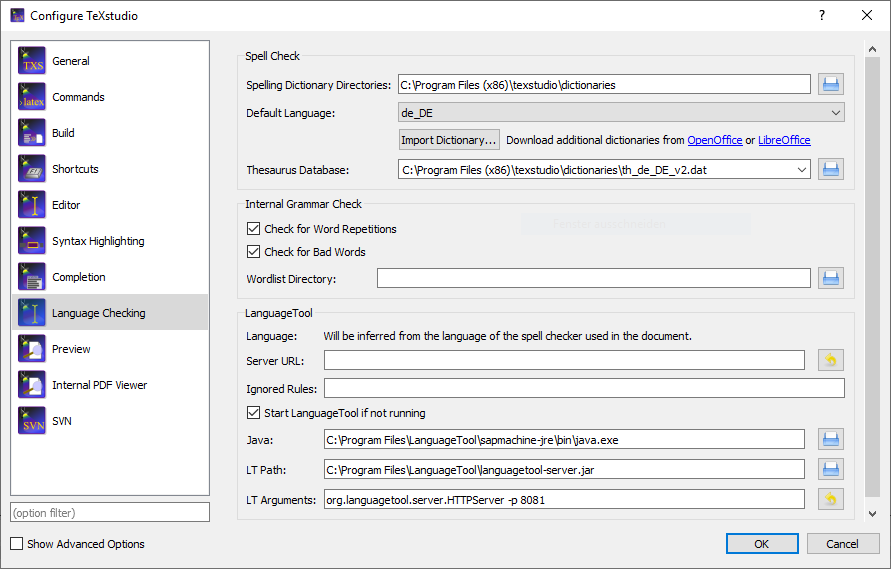
\includegraphics[width=0.9\linewidth]{example_images/texstudio-languagetool-integration}
	\caption[Settings for integrating LanguageTool with TexStudio on ISW computers]{}
	\label{fig:texstudio-languagetool-integration}
\end{figure}

\section{Version control}
\label{sec:version_control}
Whenever working on a document, it is desirable to have some sort of version control. For this task, \ac{ISW} provides a gitlab server found at \url{https://git.isw.uni-stuttgart.de/}. Once you are logged in to gitlab, you can create your own repository for tracking your thesis files. A \texttt{.gitignore} file is necessary to not track all changes to automatically generated files. You may use the \texttt{.gitignore} provided by this template. Again, if \texttt{git} is not installed on your \ac{ISW}-machine, you can install it using OPSI software-on-demand.

You can achieve a rudimentary integration with TeXstudio by defining macros such as the git commit macro shown in \autoref{lst:git_commit}. Note that macros can also be called by using shortcuts.

\begin{lstlisting}[caption={\texttt{git commit} macro}, label={lst:git_commit}]
%SCRIPT
dialog = new UniversalInputDialog()
dialog.setWindowTitle("Git commit")
dialog.add("", "Message", "comment")
dialog.add(false, "Commit all files","allfiles")
if (dialog.exec() != null) {
comment = dialog.get("comment")
if ((dialog.get("allfiles")) == true){
buildManager.runCommand(
"git commit -a -m \"" + comment + "\"", editor.fileName())
}else{
buildManager.runCommand(
"git commit " + editor.fileName() + " -m \"" + comment +
"\"", editor.fileName())
}
}
\end{lstlisting}


    % ********************************************************************
    % End of contents
    % ********************************************************************
    
    \cleardoublepage
    \printbibliography
    
    \cleardoublepage
    \addchap{List of Acronyms} % Abkürzungsverzeichnis


\begin{acronym}[SPS] % longest acronym in [...] for spacing
    % \acro{short}{long}
    % \acroextra{...} wird nur im Abkürzungsverzeichnis ausgegeben.
    \acro{ISW}{Institut für Steuerungstechnik der Werkzeugmaschinen und Fertigungseinrichtungen \acroextra{der Universität Stuttgart}}
    \acro{SPS}{Speicherprogrammierbare Steuerung}
    % acrodefplural, wenn eine Pluralform benötigt wird (Standard: angehängtes "s" aus dem Englischen)
    % \acrodefplural{acroKey}[plural short]{plural long}
    \acrodefplural{SPS}[SPS]{Speicherprogrammierbare Steuerungen}
    \acro{NDA}{Non-Disclosure Agreement}
    \acro{IPC}{Inter-Process Communication}
    \acro{QoS}{Quality of Service}
    \acro{RPC}{Remote Procedure Call}
    \acro{OS}{Operating System}
    \acro{HRTS}{Hard Real-Time System}
    \acro{SRTS}{Soft Real-Time System}
    \acro{RTOS}{Real-Time Operating System}
    \acro{RTS}{Real-Time System}
    \acro{CAS}{Compare and Swap}
    \acro{DWCAS}{Double-Width Compare and Swap}
    \acro{DCAS}{Double Compare and Swap}
    \acro{FIFO}{First In First Out}
    \acro{LIFO}{Last In First Out}
    \acro{MPMC}{Multi Producer Multi Consumer}
    \acro{MPSC}{Multi Producer Single Consumer}
    \acro{SPMC}{Single Producer Multi Consumer}
    \acro{SPSC}{Single Producer Single Consumer}
    \acro{Alg.}{Algorithm}
    \acro{FAA}{Fetch and Add}
    \acro{FAS}{Fetch and Store}
    \acro{LL/SC}{Load-Linked and Store-Conditional}
    \acro{LL}{Load-Linked}
    \acro{SC}{Store-Conditional}
    \acro{VL}{Validate-Link}
    \acro{FFQ}{FastForward Queue}
    \acro{IFFQ}{Improved FastForward Queue}
    \acro{BIFFQ}{Batched Improved FastForward Queue}
    \acro{uSPSC}{Unbounded Single Producer Single Consumer}
    \acro{dSPSC}{Dynamic Single Producer Single Consumer}
    \acro{mSPSC}{MultiPush Single Producer Single Consumer}
    \acro{BLQ}{Batched Lamport Queue}
    \acro{LLQ}{Lazy Lamport Queue}
    \acro{BLQ}{Batched Lamport Queue}
    \acro{wCQ}{Wait-Free Circular Queue}
    \acro{YMC}{Yang Mellor-Crummey}
    \acro{sCQ}{Scalable Circular Queue}
    \acro{JPQ}{Jayanti Petrovic Queue}
\end{acronym}
    
    \cleardoublepage
    \listoffigures
    
    \cleardoublepage
    \listoftables

    \cleardoublepage
    \listofalgorithms

    \cleardoublepage
    \lstlistoflistings
    
    % \cleardoublepage
\addchap{List of Symbols}

This section is optional. 
Ask your supervisor whether it is required for your thesis. 
If you have more than 10 formulas involved it probably is.

There are two ways to build a list of symbols:

\begin{itemize}
    \item If you just want to get it done, then use a \texttt{longtable} and fill your symbols in, see table below.
    \item If you want it fancy, then package \texttt{glossaries} (maybe \texttt{glossaries-extra}) may be your way to go. 
    Be warned that although it automates symbol handling (e.g. sorting and referencing of symbols), it comes with some administrative overhead. 
    You can find a discussion on different ways to achieve this \href{https://tex.stackexchange.com/a/366282}{on https://tex.stackexchange.com/a/366282}.
\end{itemize}

\begin{center}
\begin{longtable}{@{}c l p{10cm}@{}}
\toprule
Symbol & Unit & Description \\
\midrule
\endfirsthead
\multicolumn{3}{c}{\textit{List of Symbols -- continued}}\\
\toprule
Symbol & Unit & Description \\
\midrule
\endhead
\bottomrule \multicolumn{3}{r}{\textit{Continued on next page}} \\
\endfoot
\bottomrule
\endlastfoot

% start here with your symbols:
\(\psi\) & rad & Heading angle of hamster \\
\(\dot x\) & m/s & Linear velocity of hamster \\
\(\ddot x_0\) & m/s$^2$ & Initial acceleration of hamster \\
\end{longtable}
\end{center}
    
    % Appendix, if needed:
    \appendix
    \chapter{Appendix}

\section{Additional Benchmark Visualisations}
This section presents additional violin plots from the benchmark results, illustrating performance distributions for various producer and consumer configurations. These complement the main results presented in \cref{ch:results}.

\subsection{MPSC Queue Performance Distributions}\label{subsec:mpsc-violin}
The following figures show the performance distribution of MPSC queue implementations across different producer configurations:

\begin{figure}[H]
\centering
\caption{MPSC queue performance distribution with 1 producer with 500,000 Total Items}
\label{fig:mpsc-violin-1p}
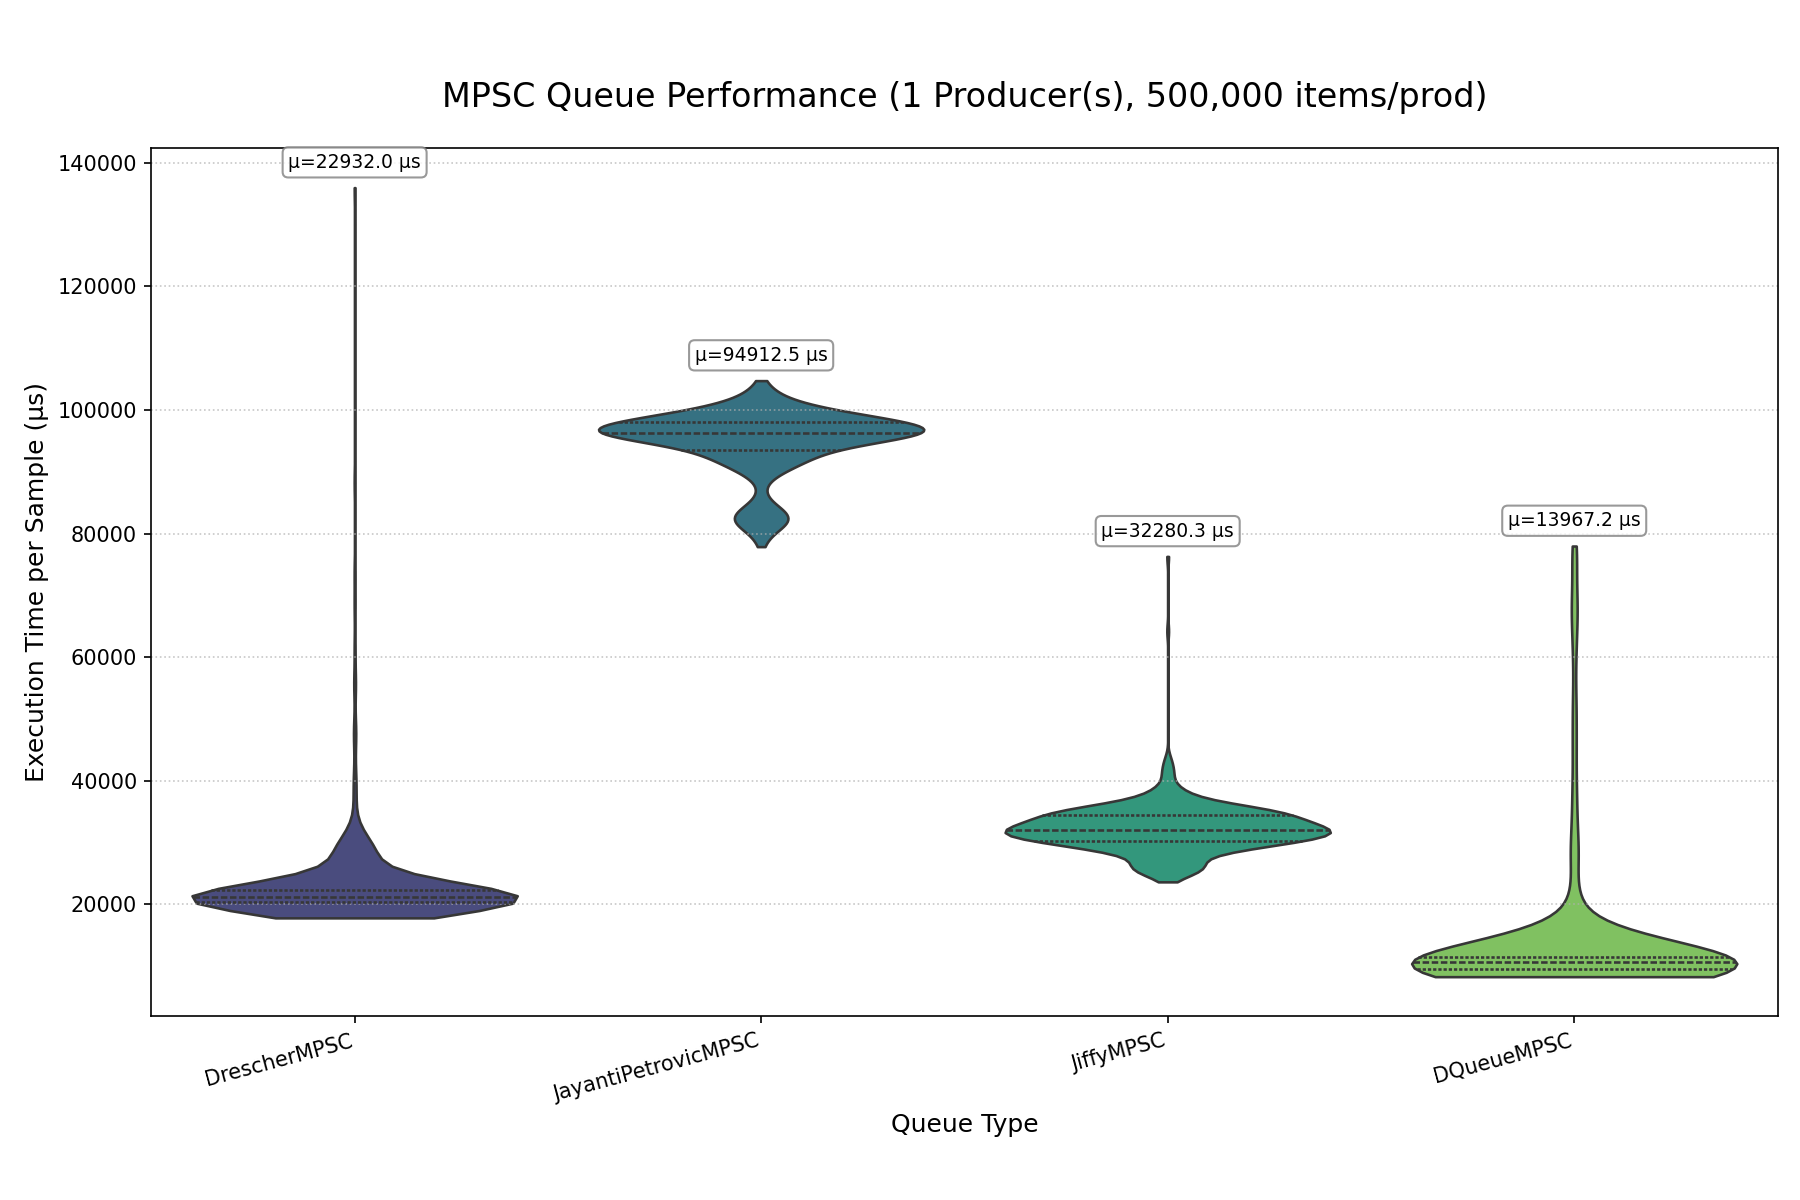
\includegraphics[width=\textwidth]{images/results/mpsc_performance_violin_1_producers.png}
\end{figure}

\begin{figure}[H]
\centering
\caption{MPSC queue performance distribution with 2 producers with 1,000,000 Total Items}
\label{fig:mpsc-violin-2p}
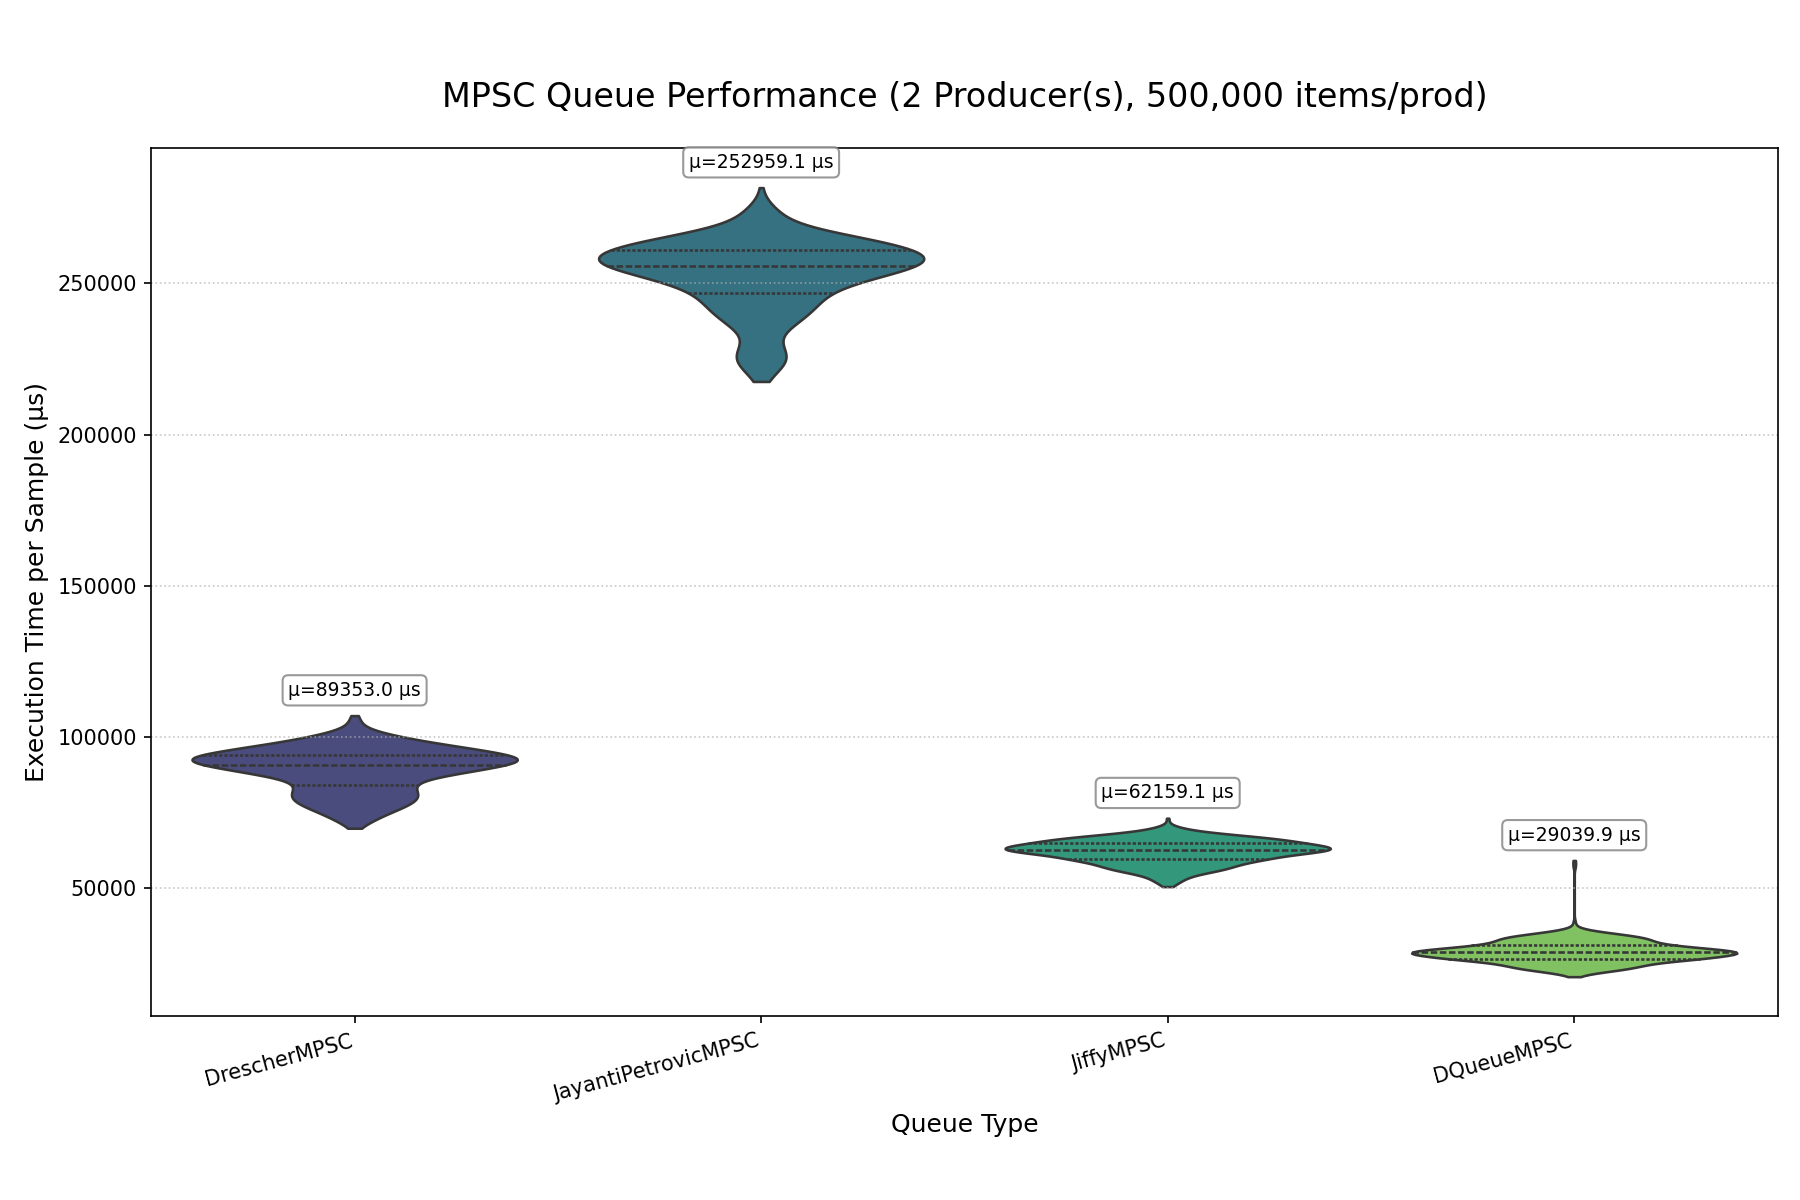
\includegraphics[width=\textwidth]{images/results/mpsc_performance_violin_2_producers.png}
\end{figure}

\begin{figure}[H]
\centering
\caption{MPSC queue performance distribution with 4 producers with 2,000,000 Total Items}
\label{fig:mpsc-violin-4p}
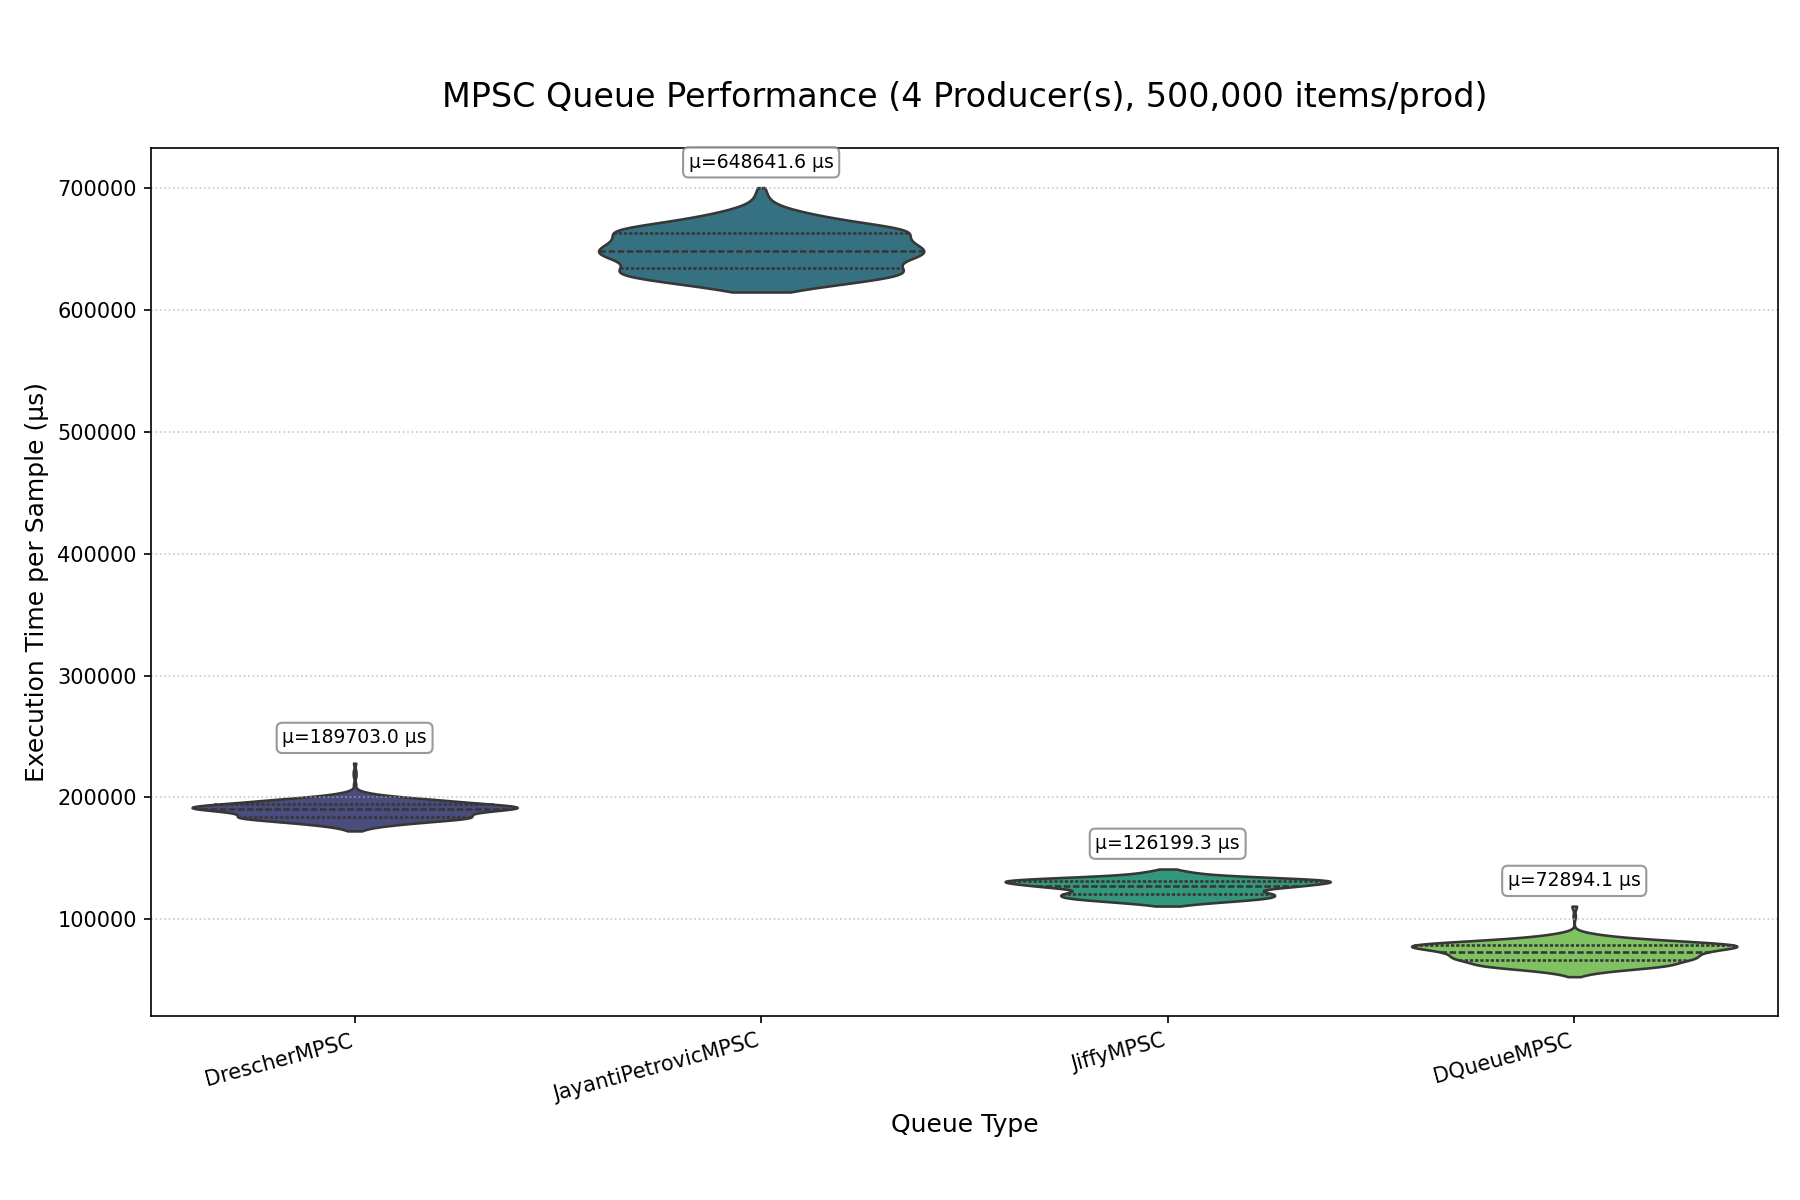
\includegraphics[width=\textwidth]{images/results/mpsc_performance_violin_4_producers.png}
\end{figure}

\begin{figure}[H]
\centering
\caption{MPSC queue performance distribution with 8 producers with 4,000,000 Total Items}
\label{fig:mpsc-violin-8p}
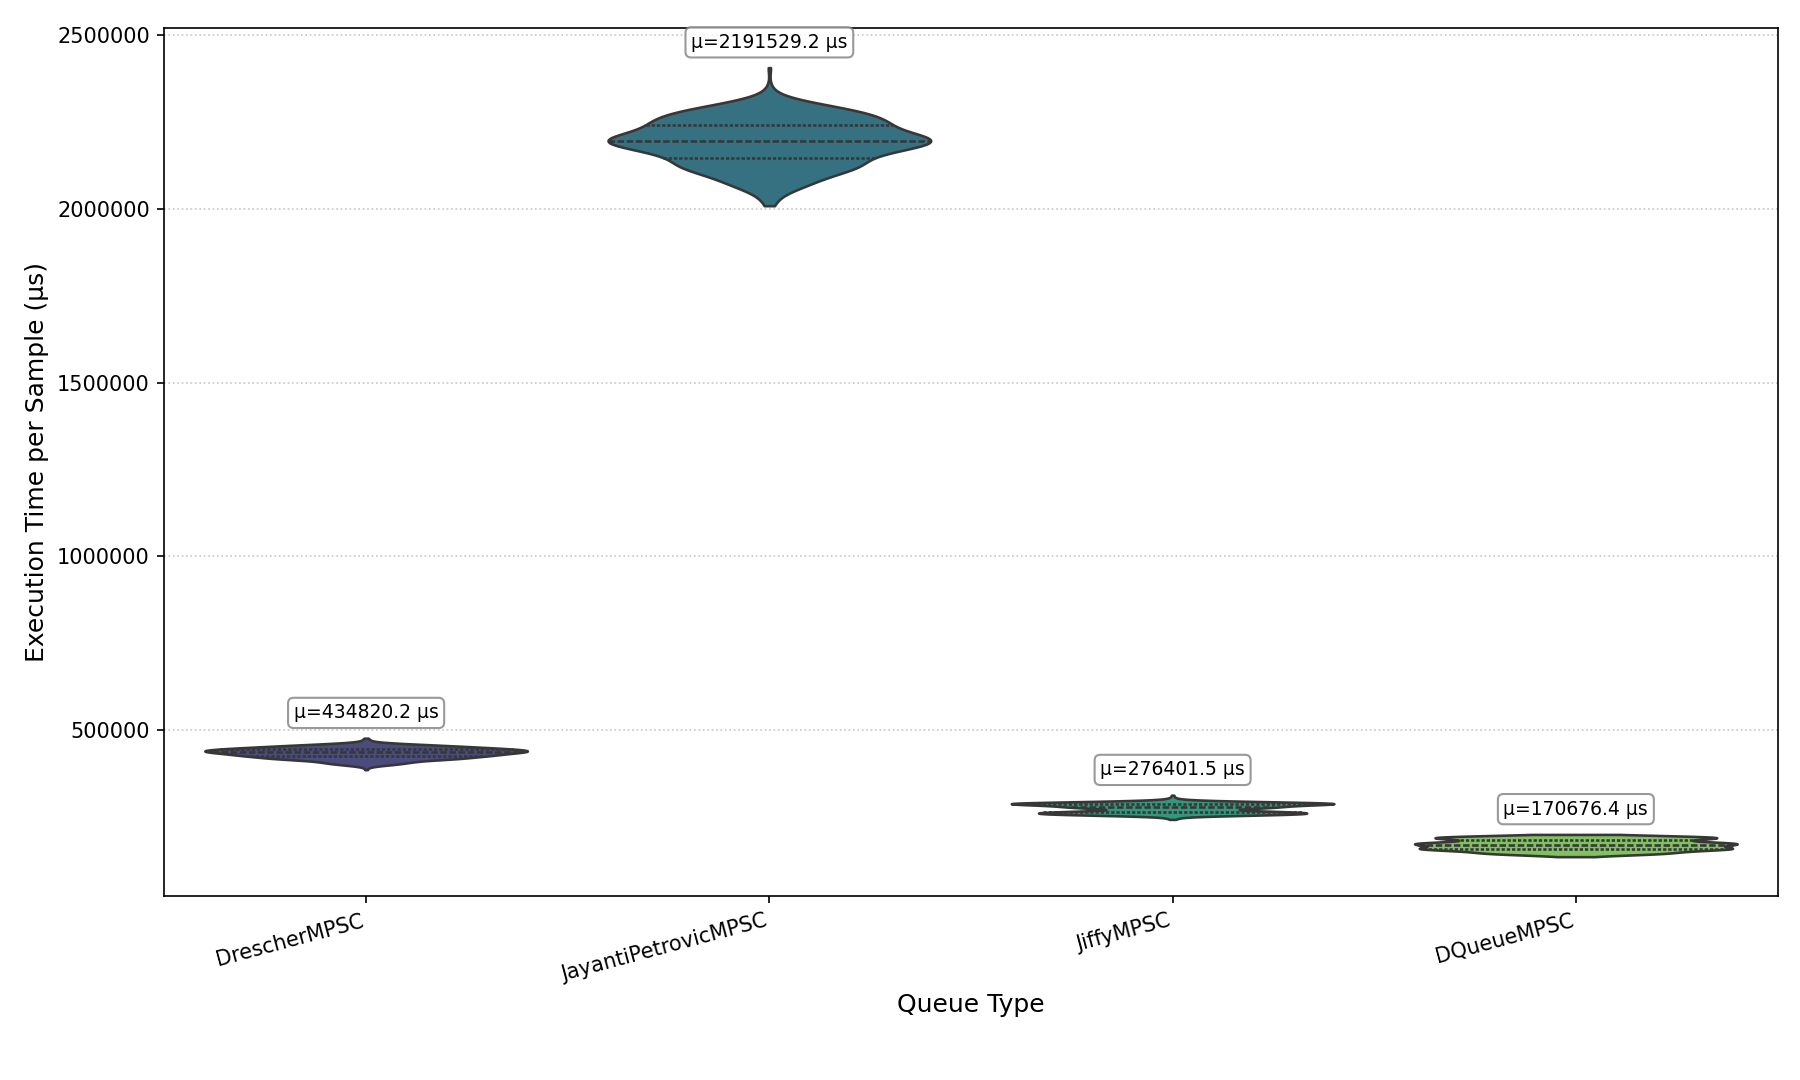
\includegraphics[width=\textwidth]{images/results/mpsc_performance_violin_8_producers.png}
\end{figure}

\subsection{MPMC Queue Performance Distributions}
The following figures show the performance distribution of MPMC queue implementations across different configurations:

\begin{figure}[H]
\centering
\caption{MPMC queue performance distribution with 1 producer and 1 consumer with 170,000 Total Items}
\label{fig:mpmc-violin-1p1c}
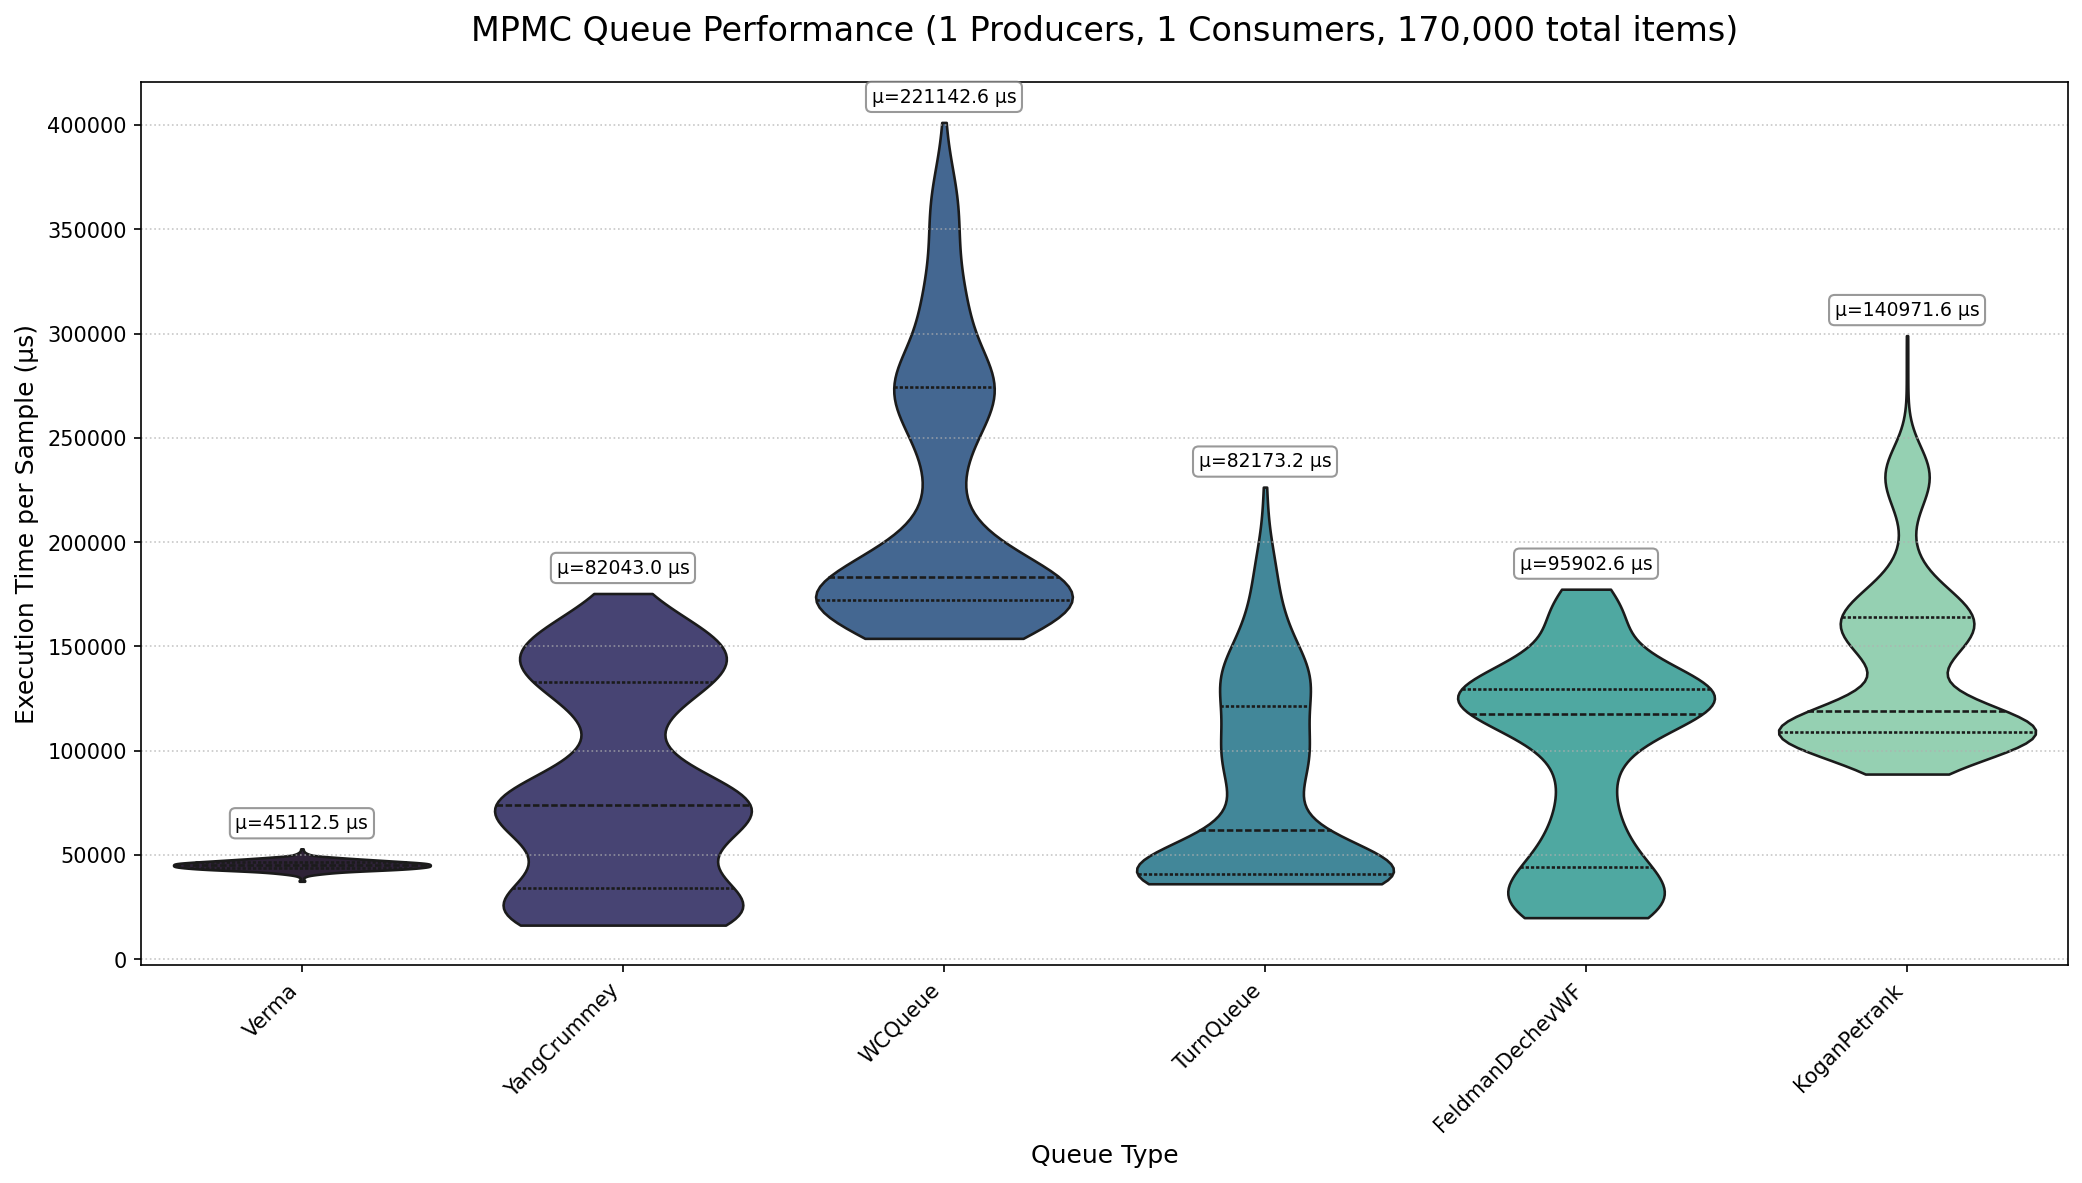
\includegraphics[width=\textwidth]{images/results/mpmc_performance_violin_1P_1C.png}
\end{figure}

\begin{figure}[H]
\centering
\caption{MPMC queue performance distribution with 2 producers and 2 consumers with 340,000 Total Items}
\label{fig:mpmc-violin-2p2c}
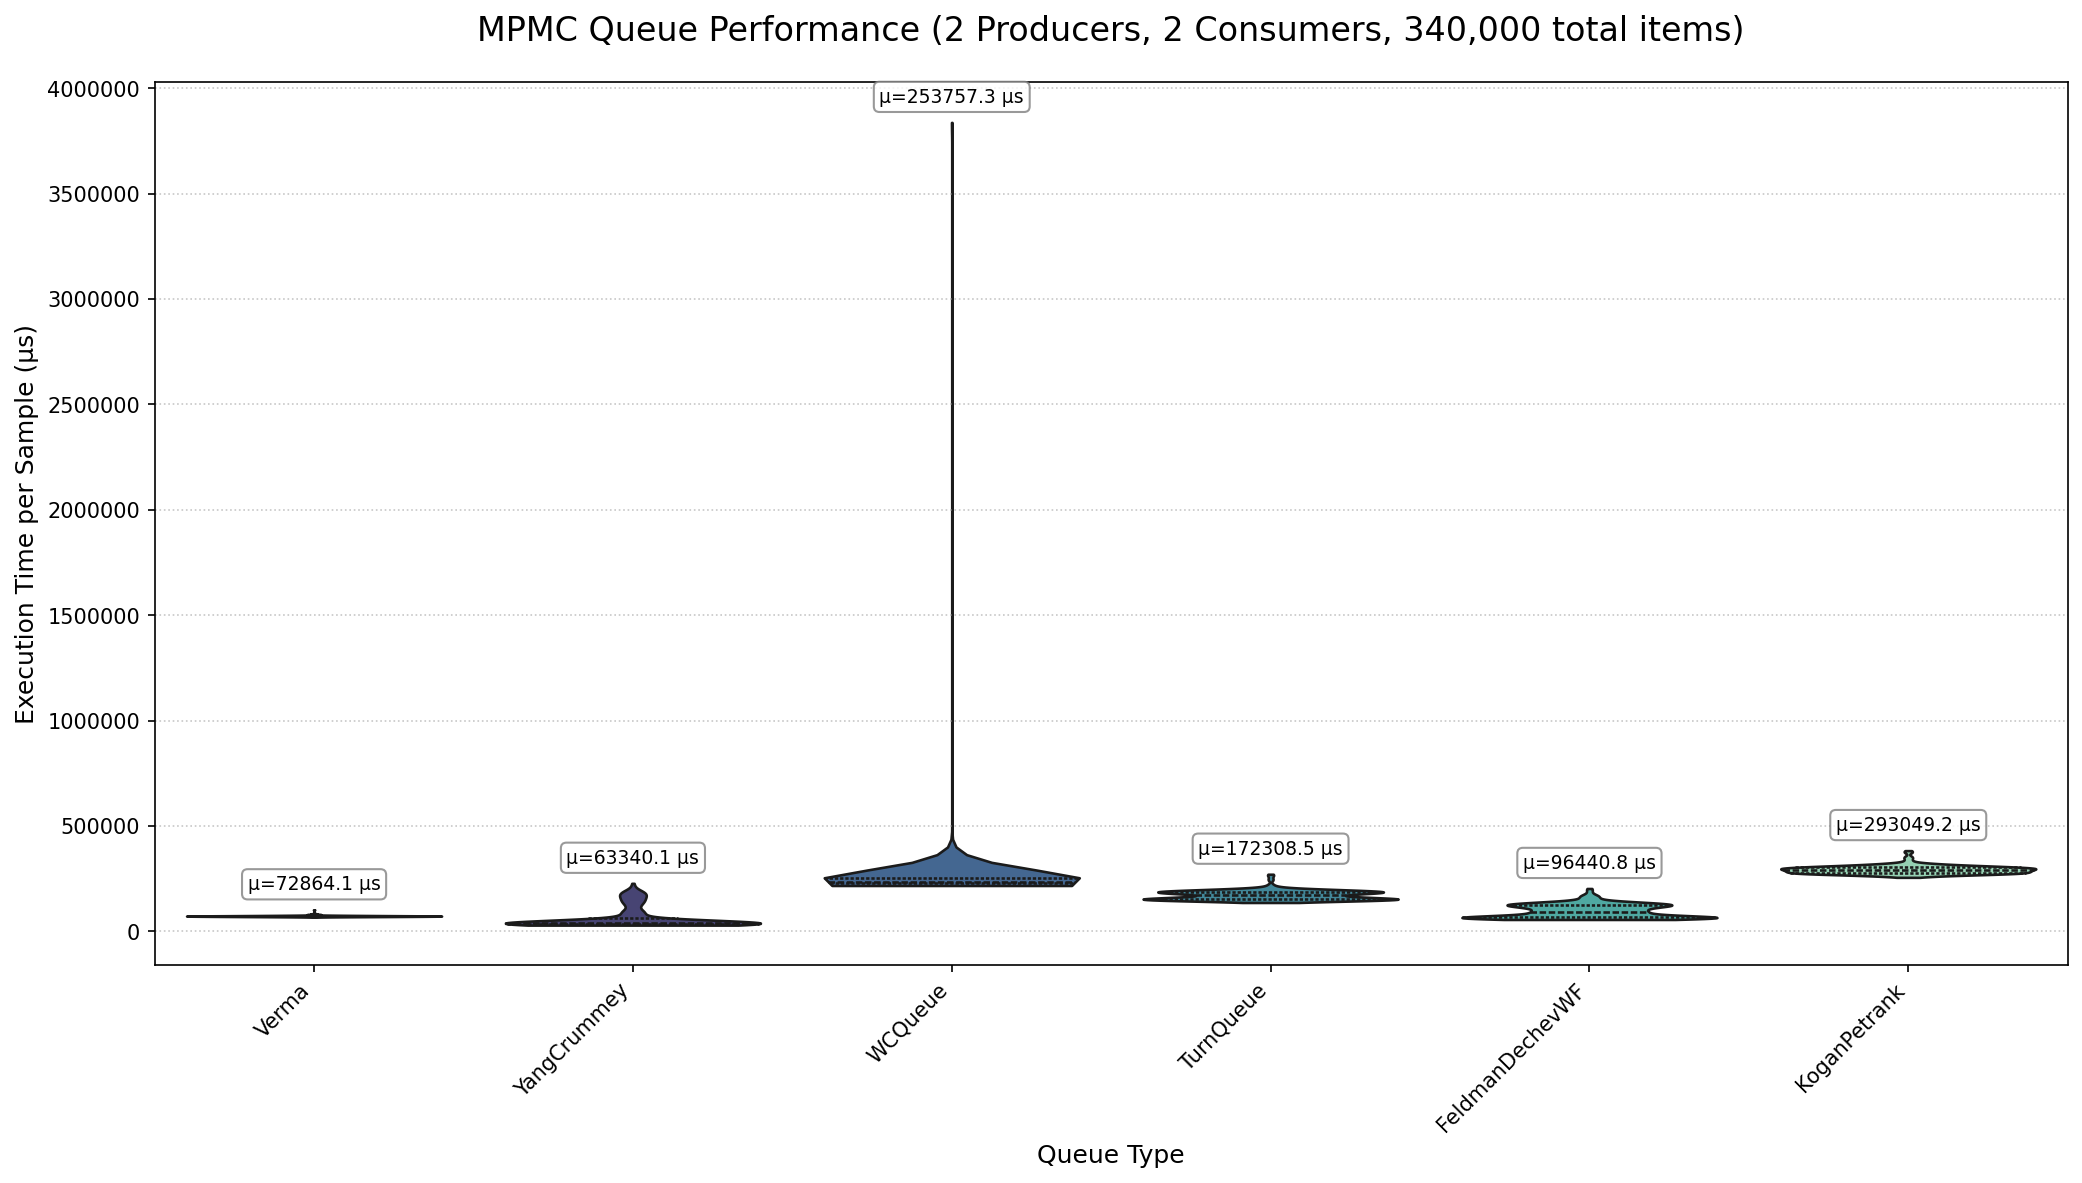
\includegraphics[width=\textwidth]{images/results/mpmc_performance_violin_2P_2C.png}
\end{figure}

\begin{figure}[H]
\centering
\caption{MPMC queue performance distribution with 4 producers and 4 consumers with 680,000 Total Items}
\label{fig:mpmc-violin-4p4c}
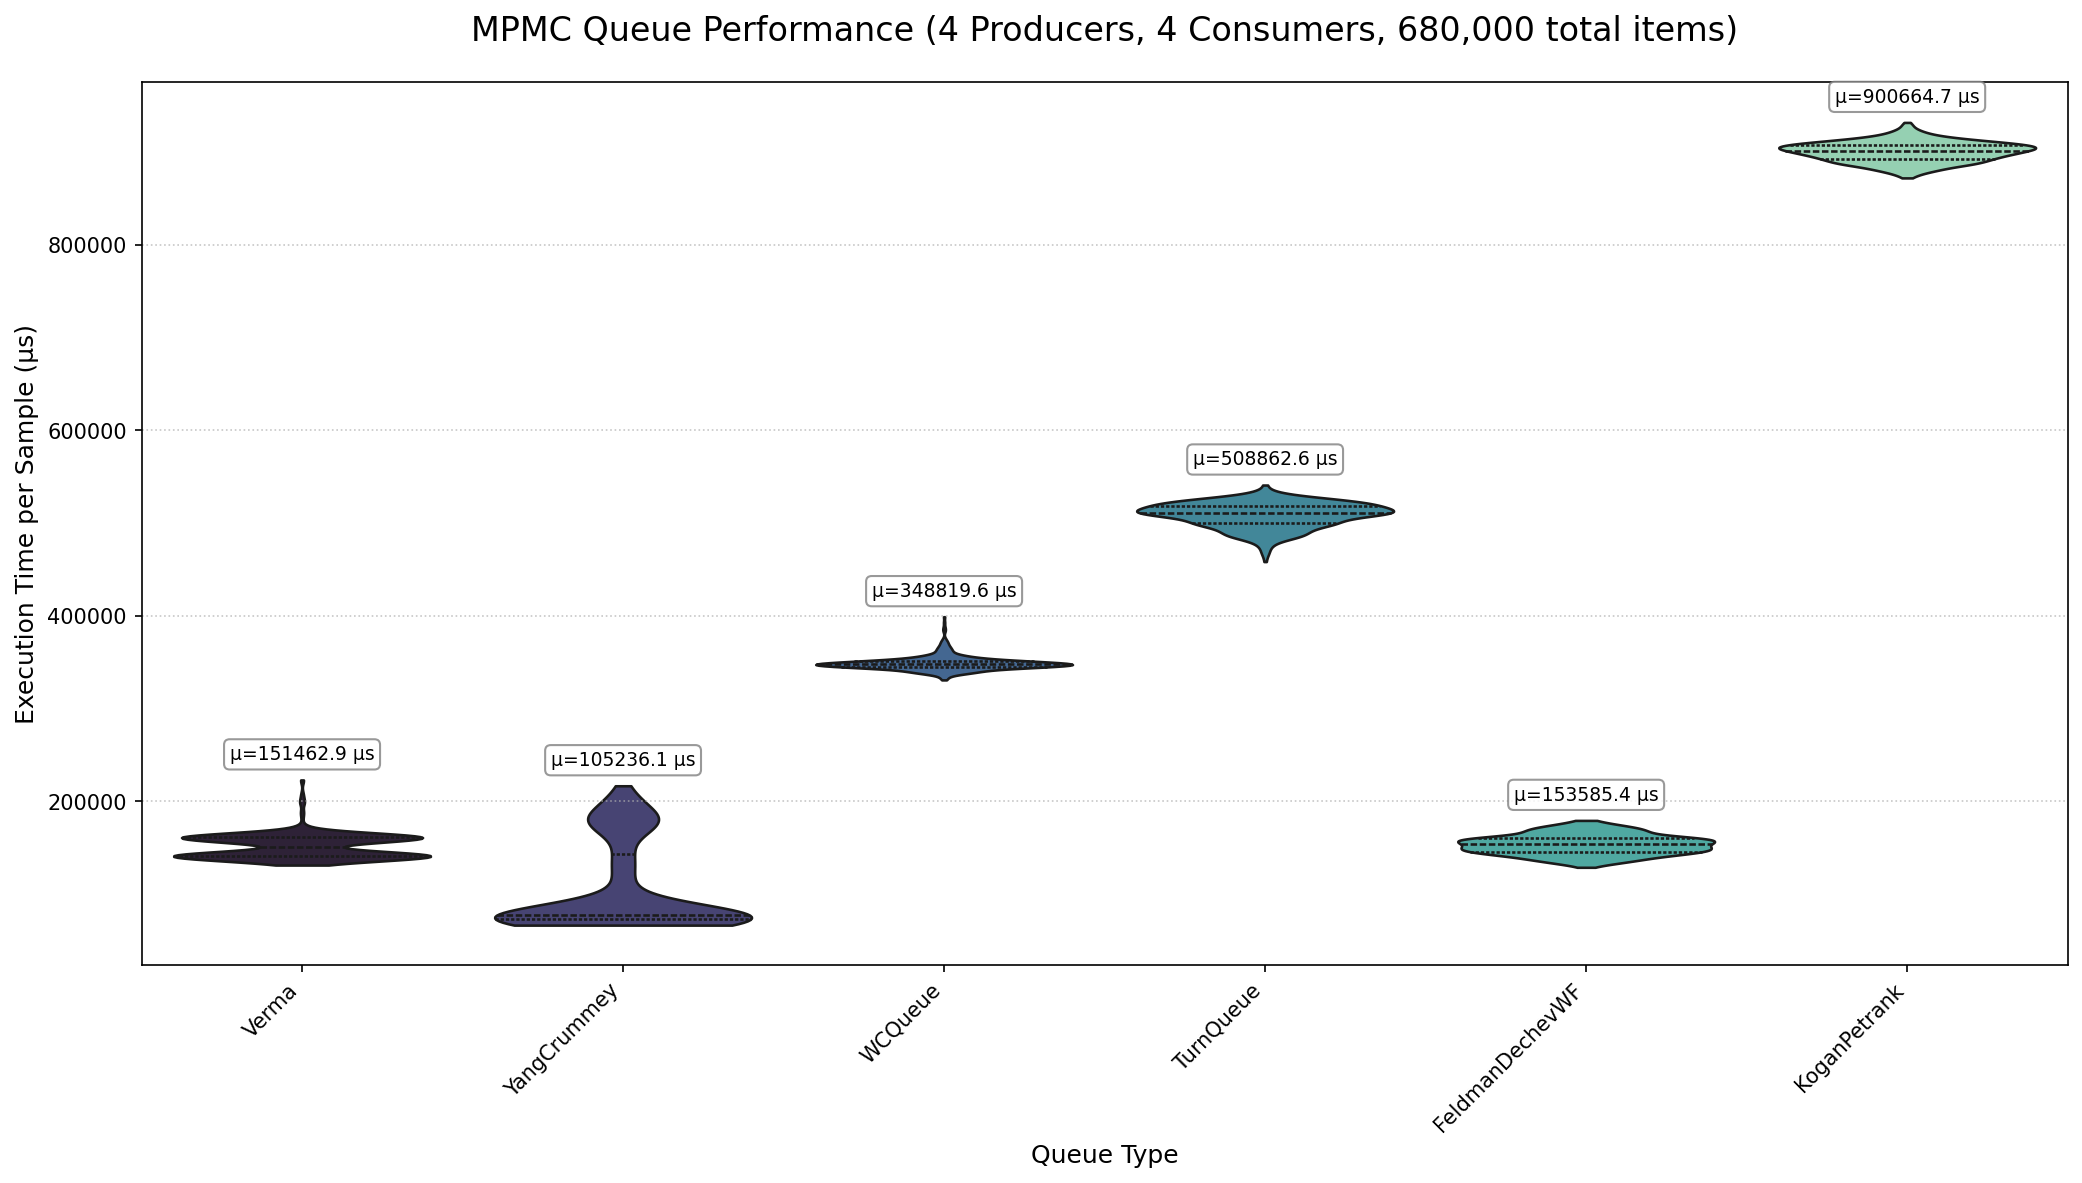
\includegraphics[width=\textwidth]{images/results/mpmc_performance_violin_4P_4C.png}
\end{figure}

\subsection{Cross-Category Performance Distributions}
The following figures show performance distributions when queues from different categories operate in various contention scenarios:

\subsubsection{Cross-Category MPSC Performance}
\begin{figure}[H]
\centering
\caption{Cross-category MPSC performance distribution with 1 producer and 1 consumer with 100,000 Total Items}
\label{fig:cross-mpsc-violin-1p}
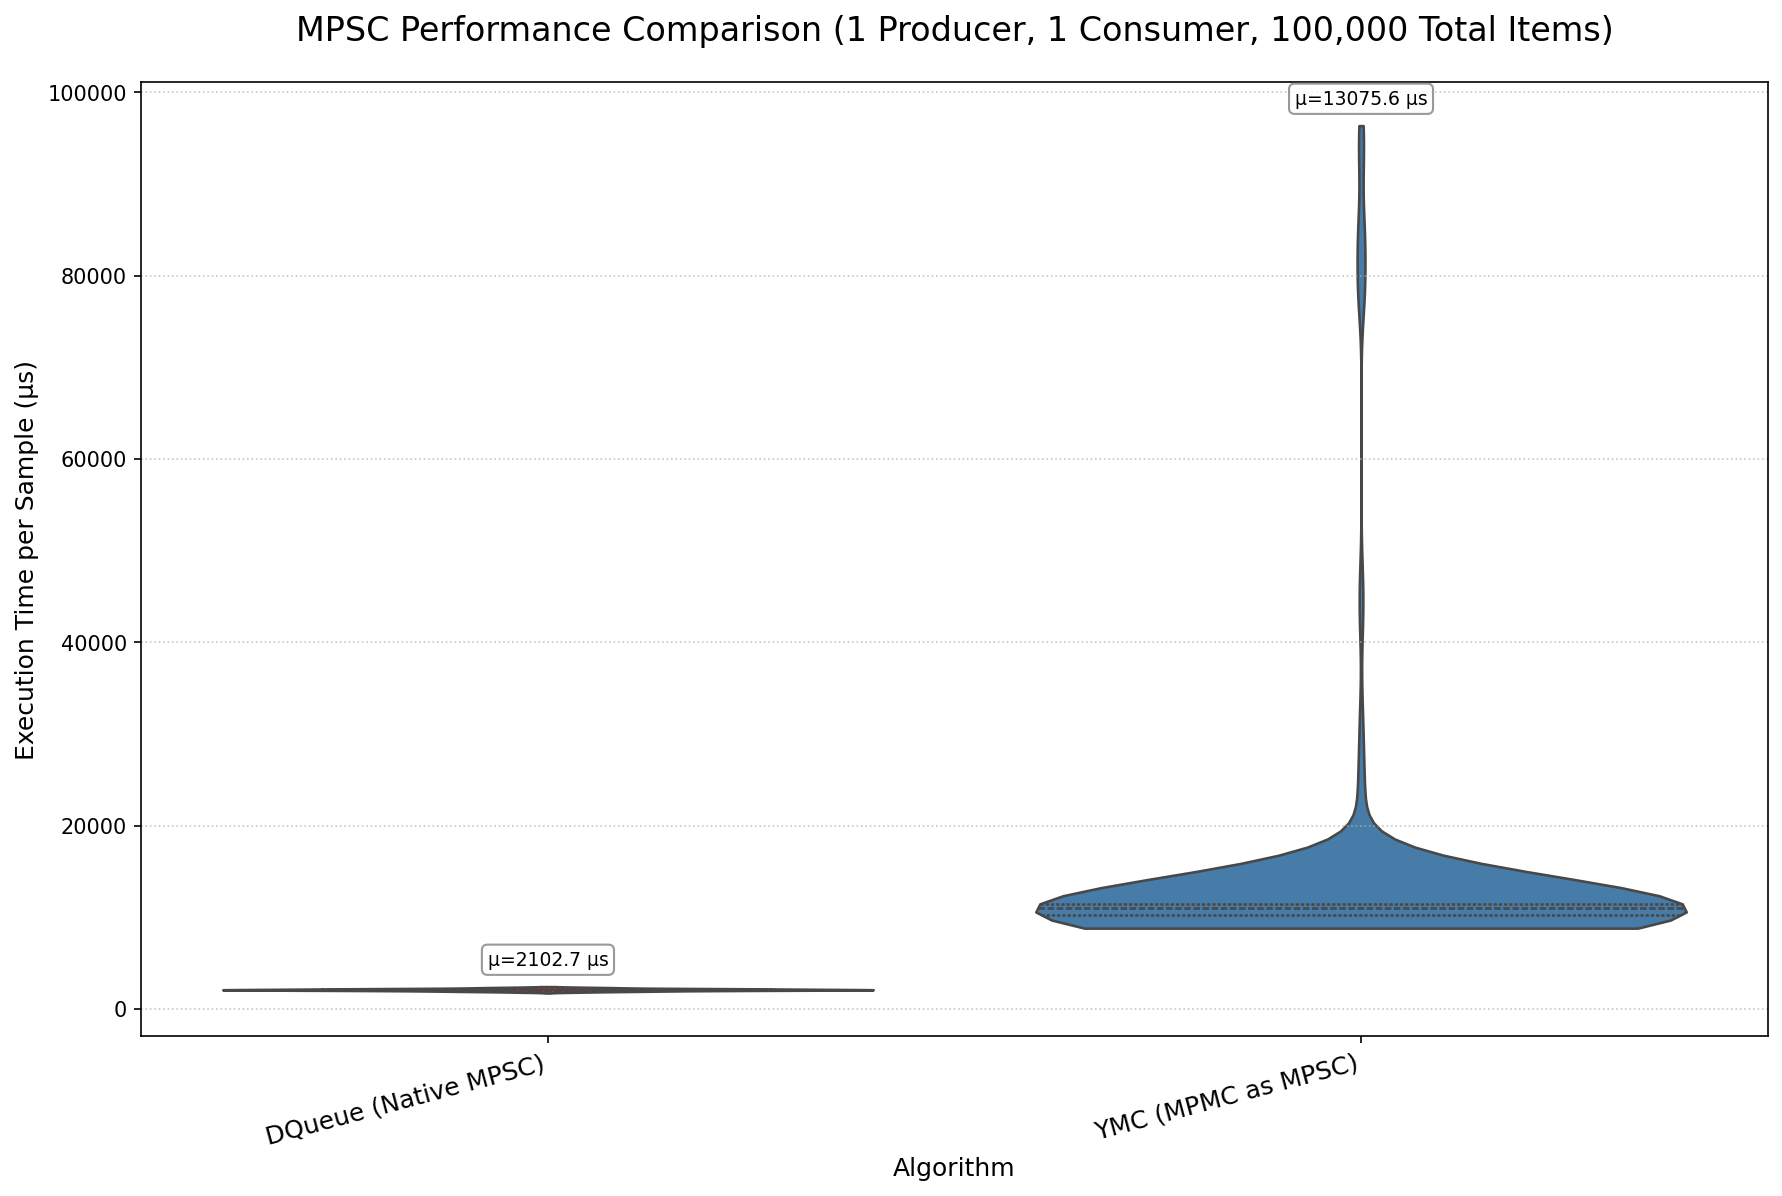
\includegraphics[width=\textwidth]{images/results/best_in_mpsc_performance_violin_1P1C.png}
\end{figure}

\begin{figure}[H]
\centering
\caption{Cross-category MPSC performance distribution with 2 producers and 1 consumer with 200,000 Total Items}
\label{fig:cross-mpsc-violin-2p}
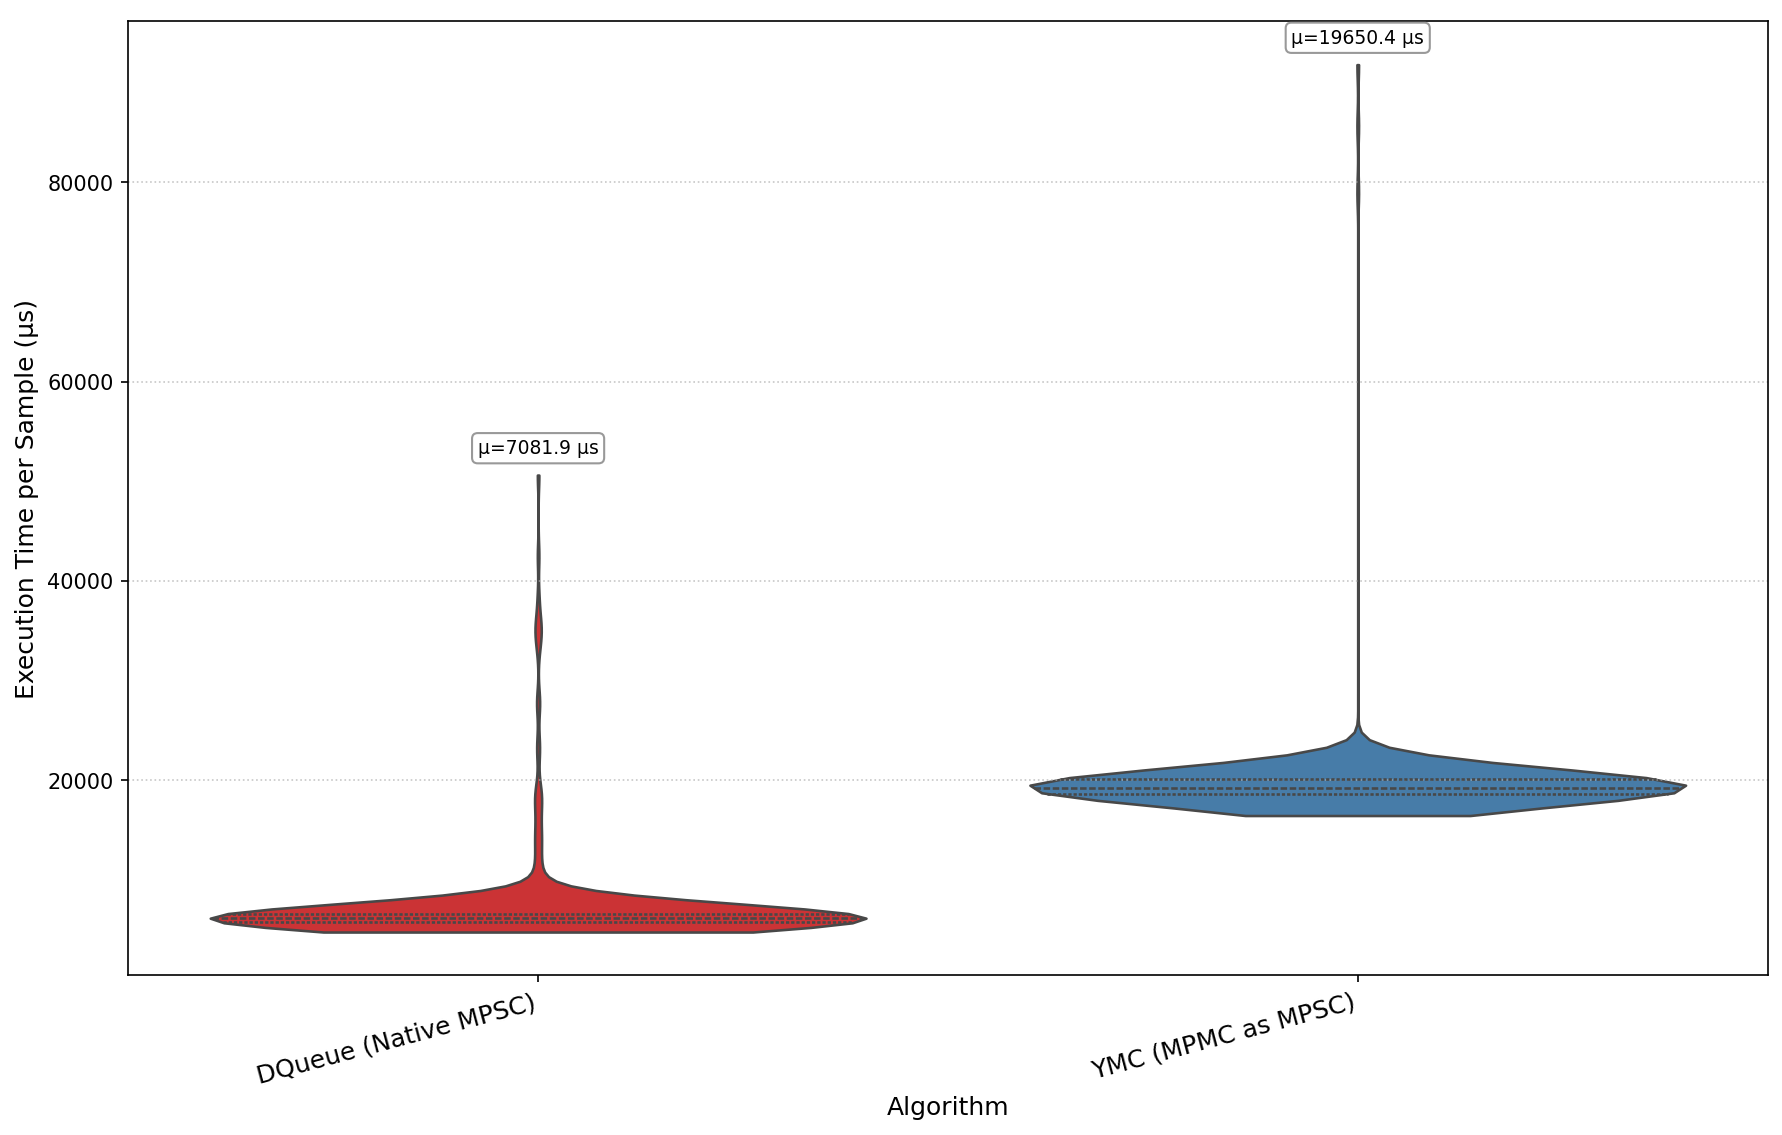
\includegraphics[width=\textwidth]{images/results/best_in_mpsc_performance_violin_2P1C.png}
\end{figure}

\begin{figure}[H]
\centering
\caption{Cross-category MPSC performance distribution with 4 producers and 1 consumer with 400,000 Total Items}
\label{fig:cross-mpsc-violin-4p}
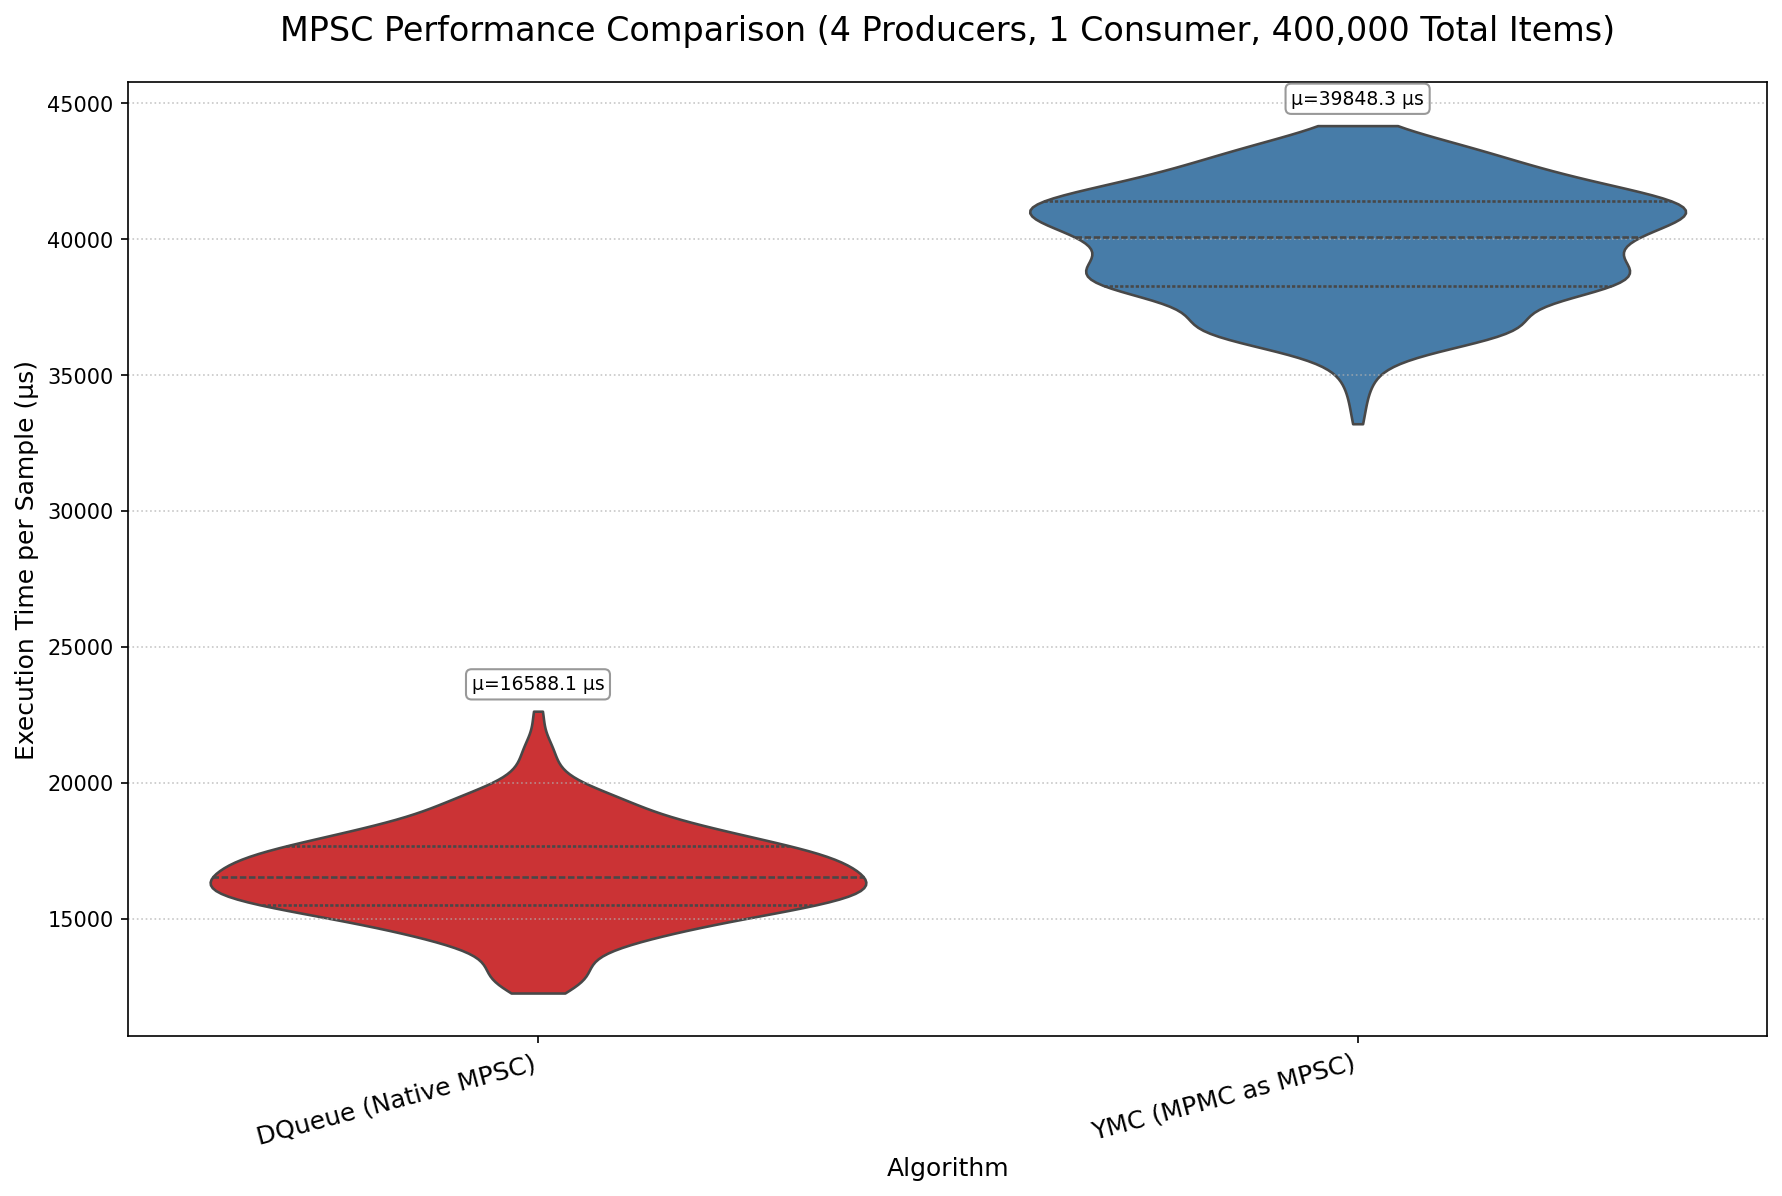
\includegraphics[width=\textwidth]{images/results/best_in_mpsc_performance_violin_4P1C.png}
\end{figure}

\begin{figure}[H]
\centering
\caption{Cross-category MPSC performance distribution with 8 producers and 1 consumer with 800,000 Total Items}
\label{fig:cross-mpsc-violin-8p}
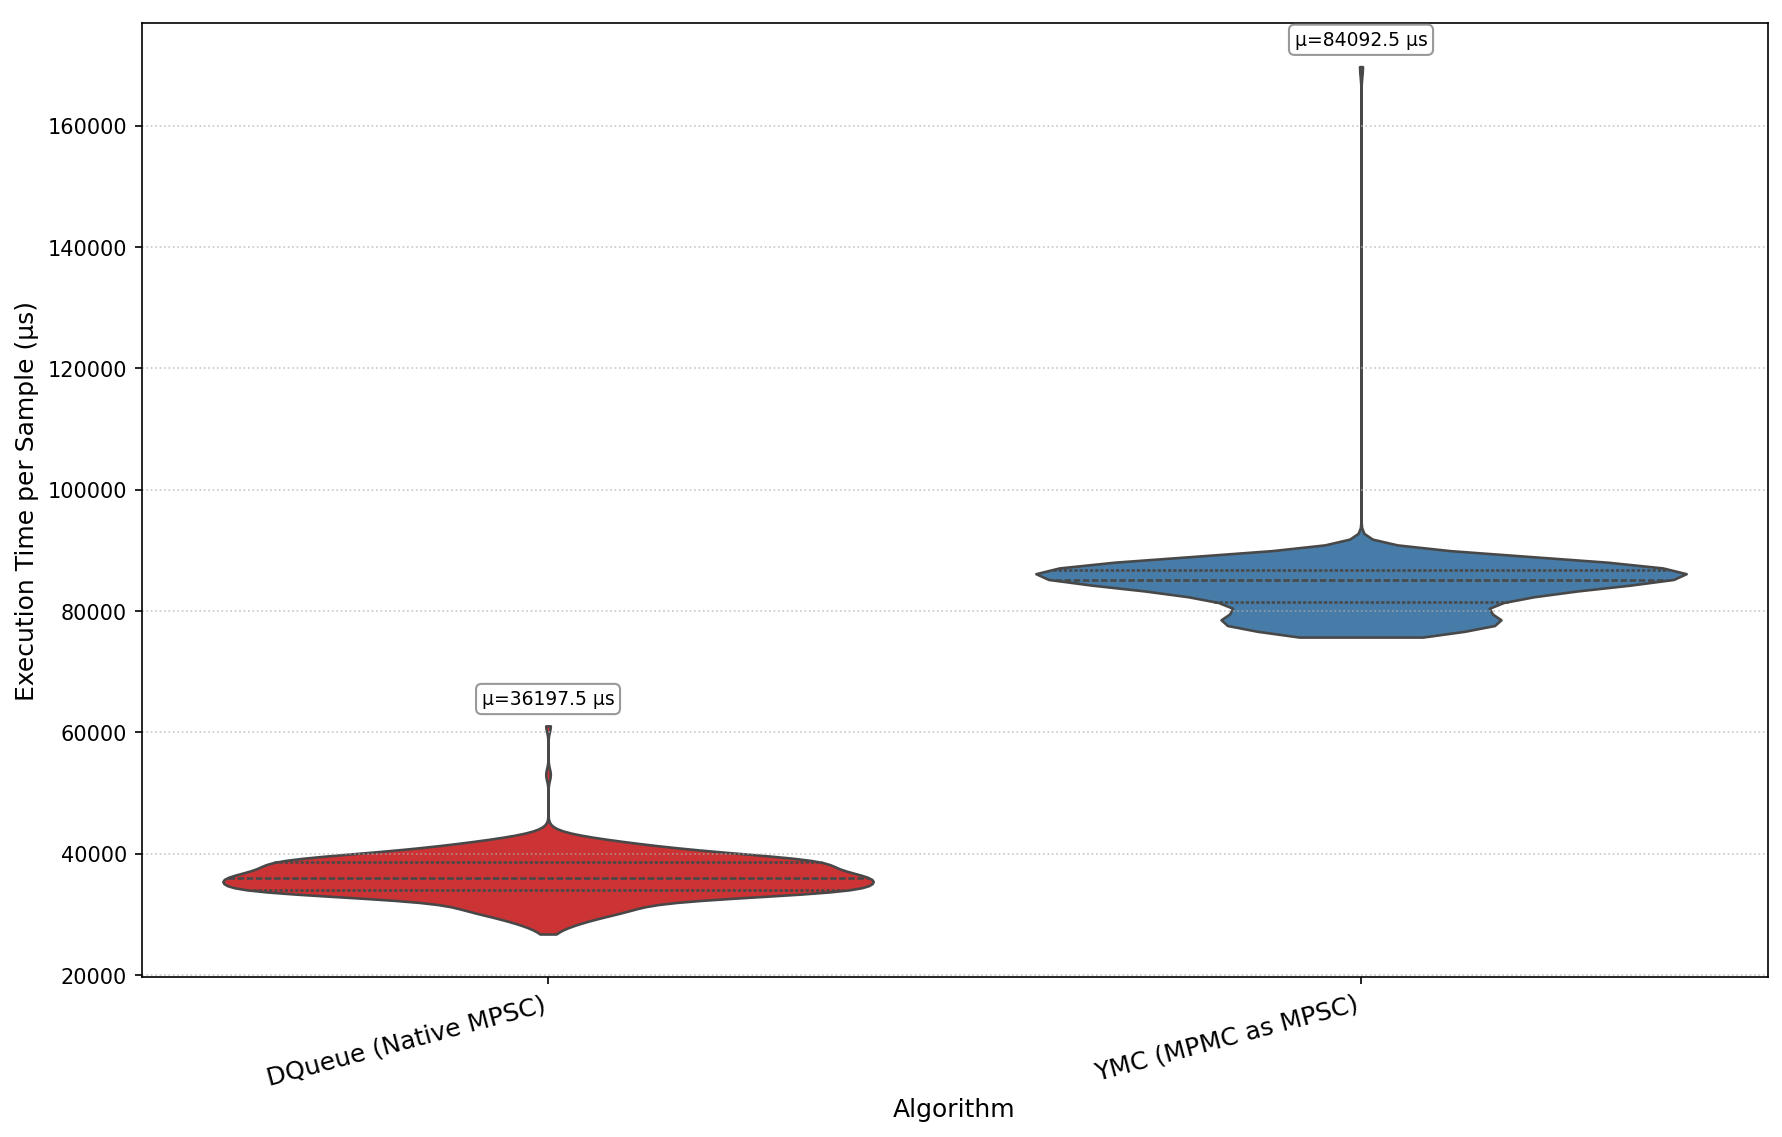
\includegraphics[width=\textwidth]{images/results/best_in_mpsc_performance_violin_8P1C.png}
\end{figure}

\subsubsection{Cross-Category SPMC Performance}
\begin{figure}[H]
\centering
\caption{Cross-category SPMC performance distribution with 1 producer and 1 consumer with 100,000 Total Items}
\label{fig:cross-spmc-violin-1c}
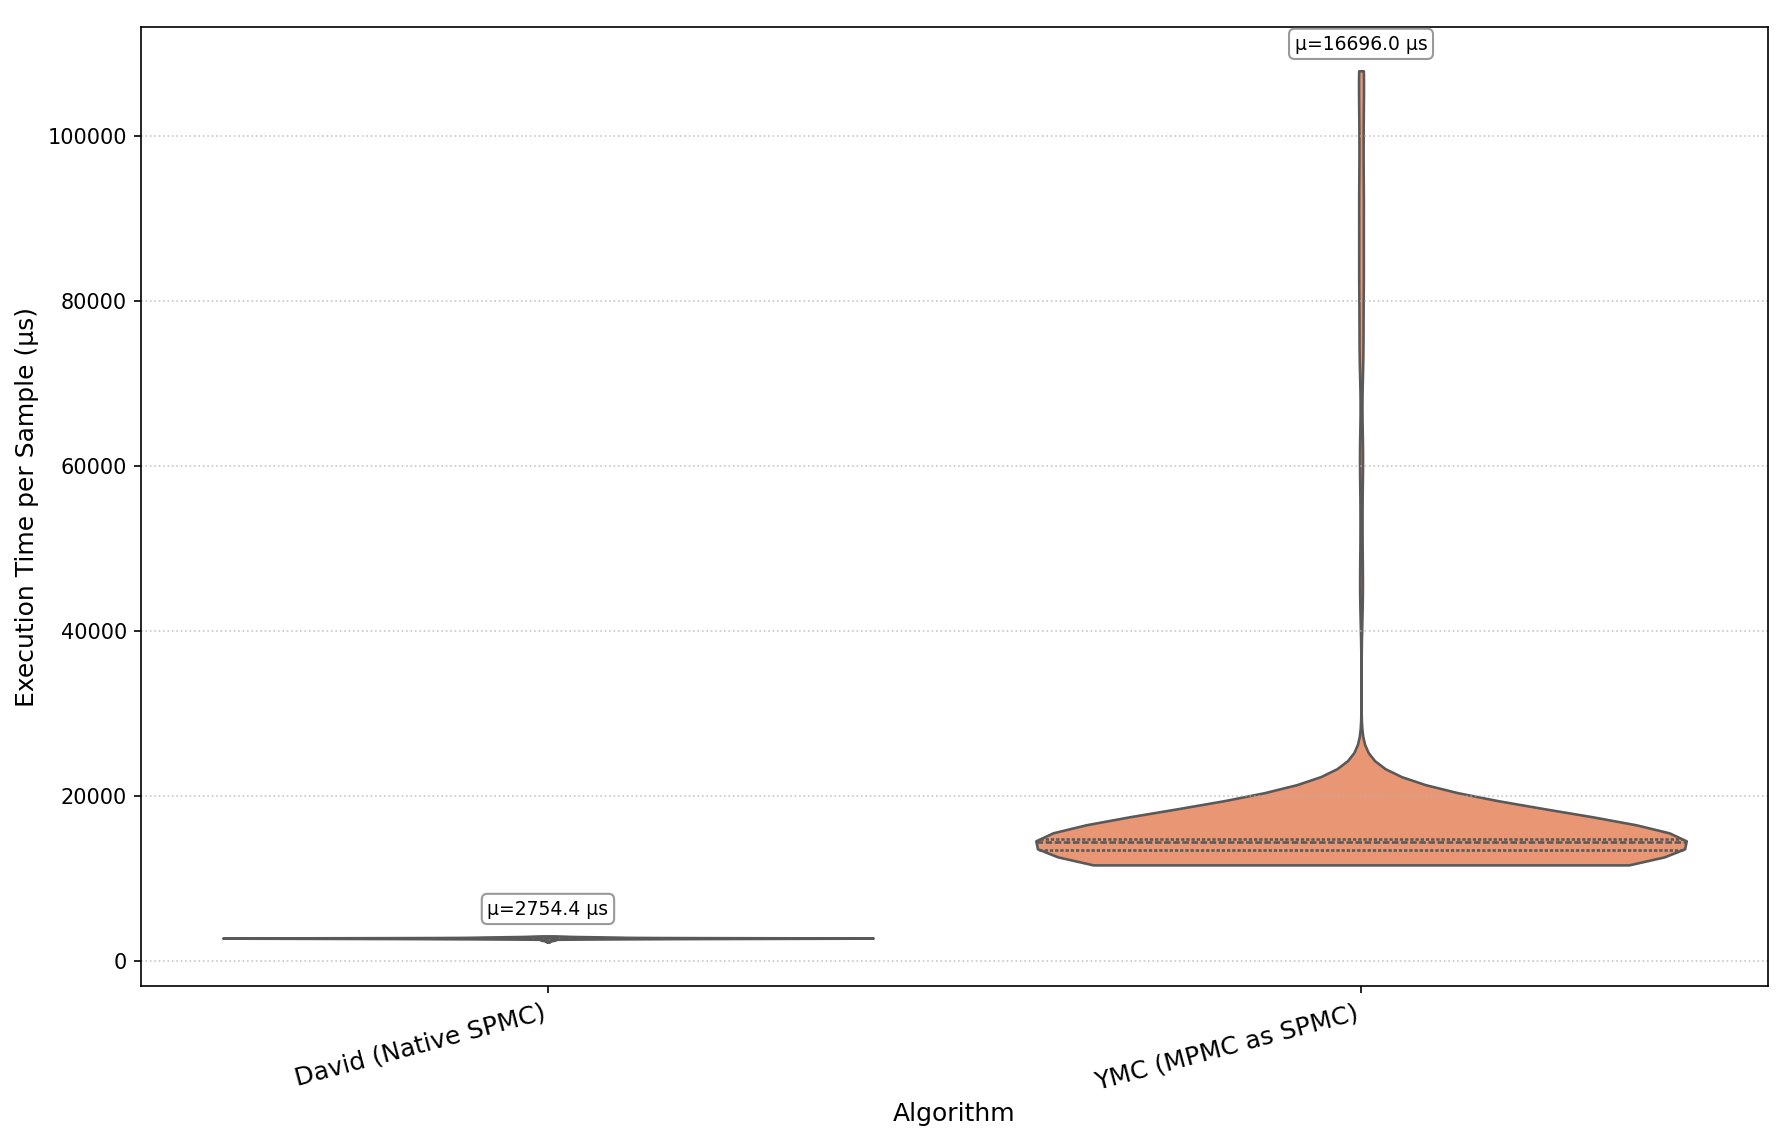
\includegraphics[width=\textwidth]{images/results/best_in_spmc_performance_violin_1P1C.png}
\end{figure}

\begin{figure}[H]
\centering
\caption{Cross-category SPMC performance distribution with 1 producer and 2 consumers with 200,000 Total Items}
\label{fig:cross-spmc-violin-2c}
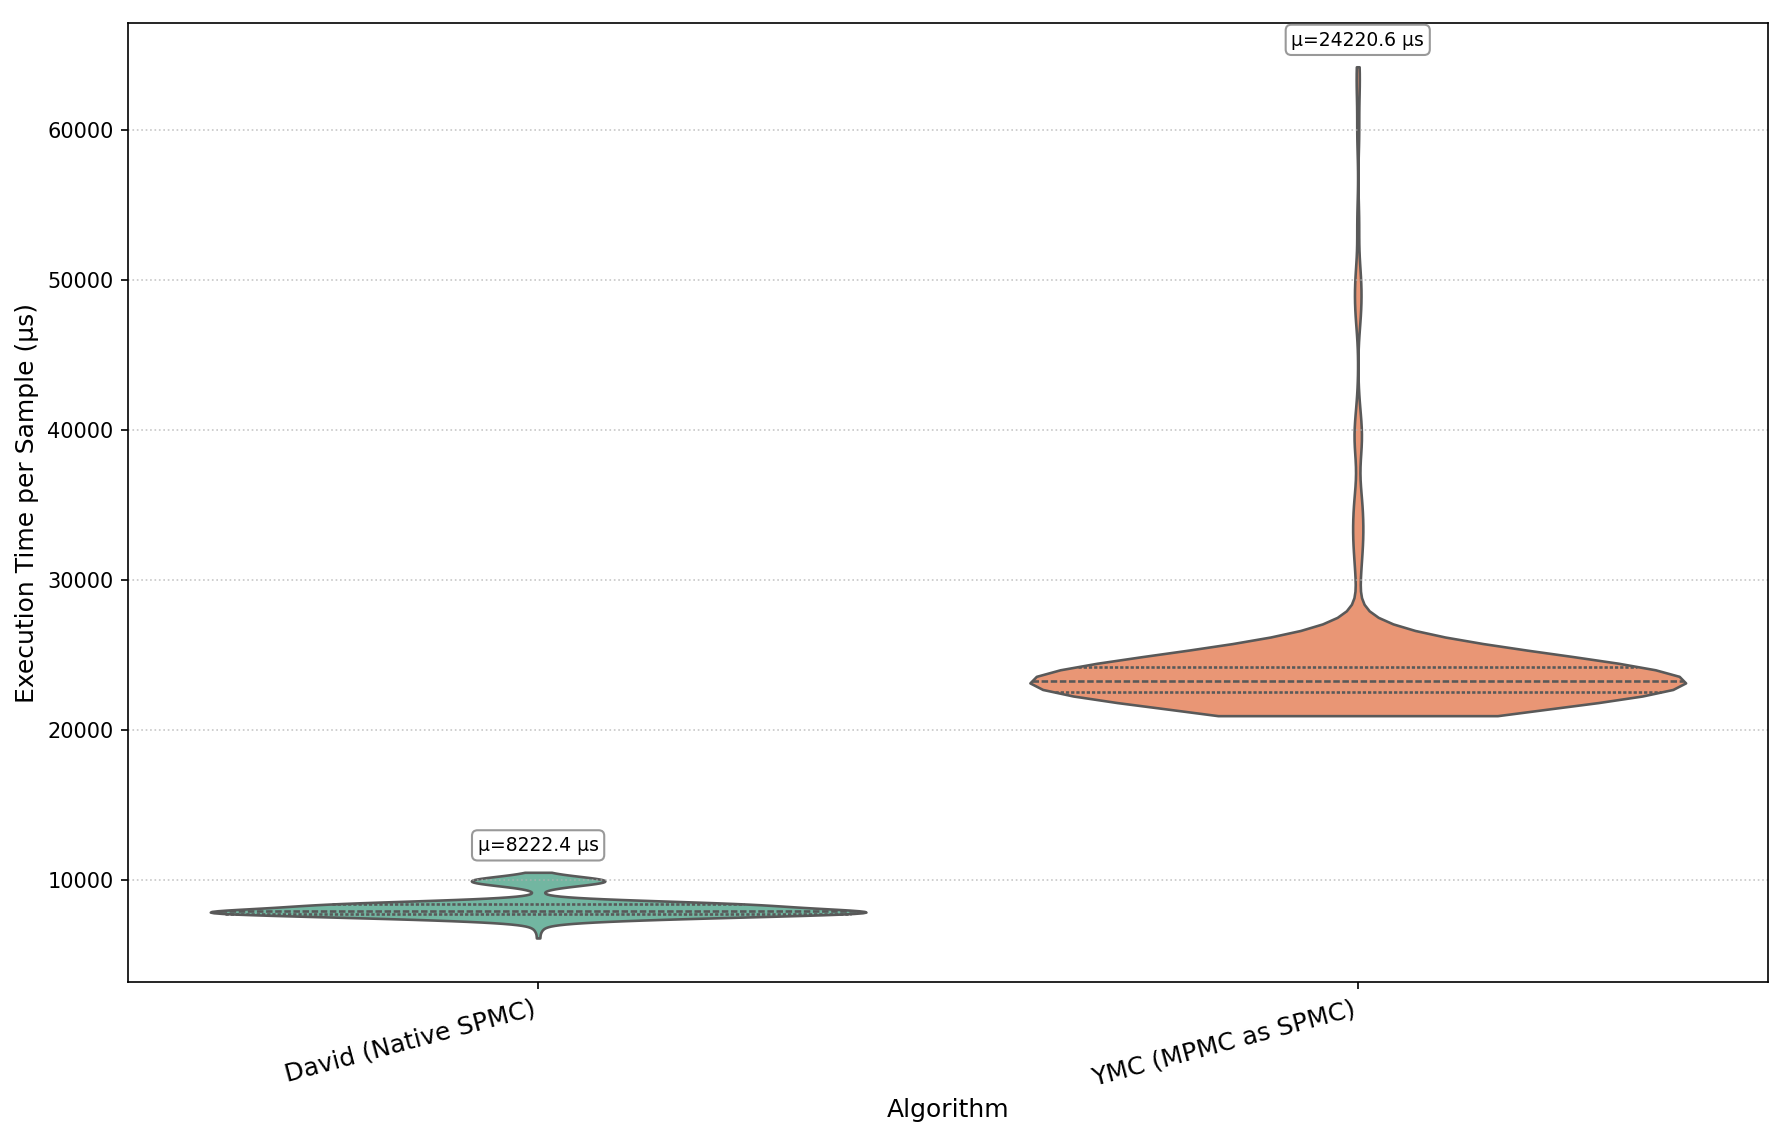
\includegraphics[width=\textwidth]{images/results/best_in_spmc_performance_violin_1P2C.png}
\end{figure}

\begin{figure}[H]
\centering
\caption{Cross-category SPMC performance distribution with 1 producer and 4 consumers with 400,000 Total Items}
\label{fig:cross-spmc-violin-4c}
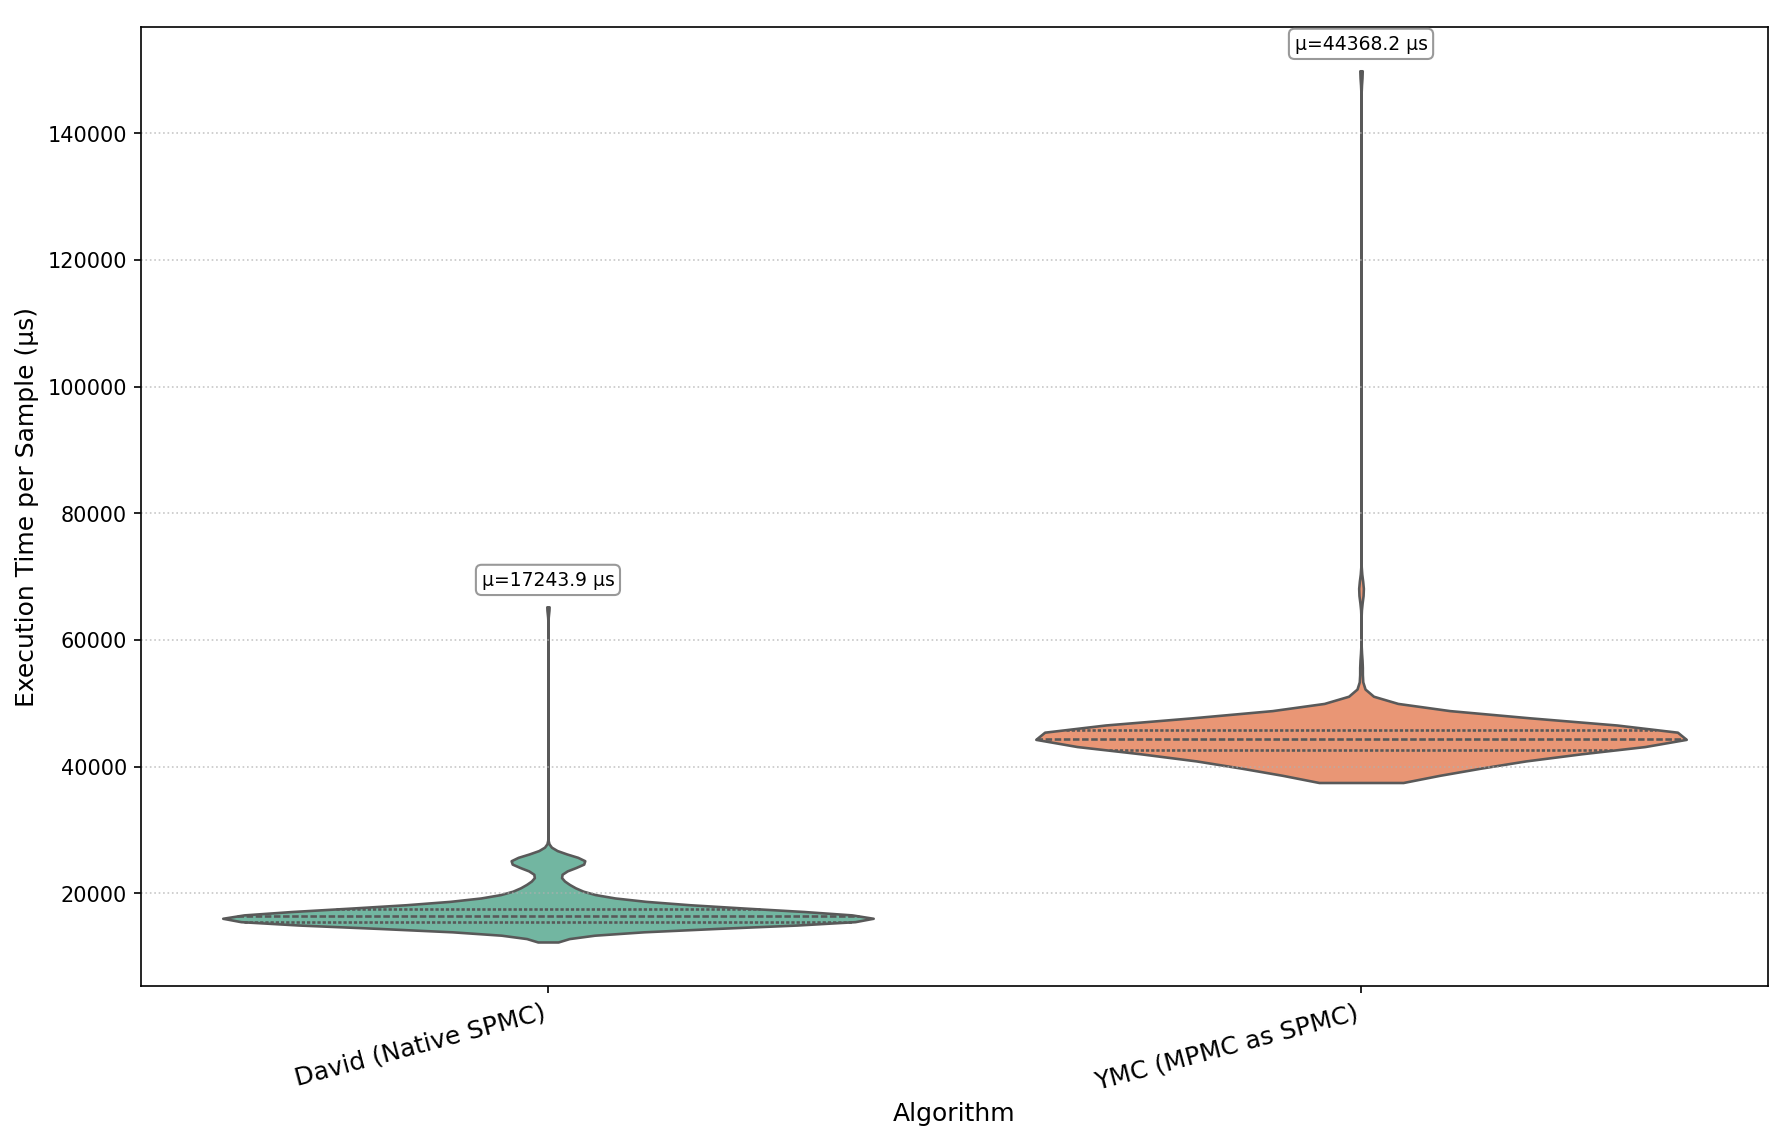
\includegraphics[width=\textwidth]{images/results/best_in_spmc_performance_violin_1P4C.png}
\end{figure}

\begin{figure}[H]
\centering
\caption{Cross-category SPMC performance distribution with 1 producer and 8 consumers with 800,000 Total Items}
\label{fig:cross-spmc-violin-8c}
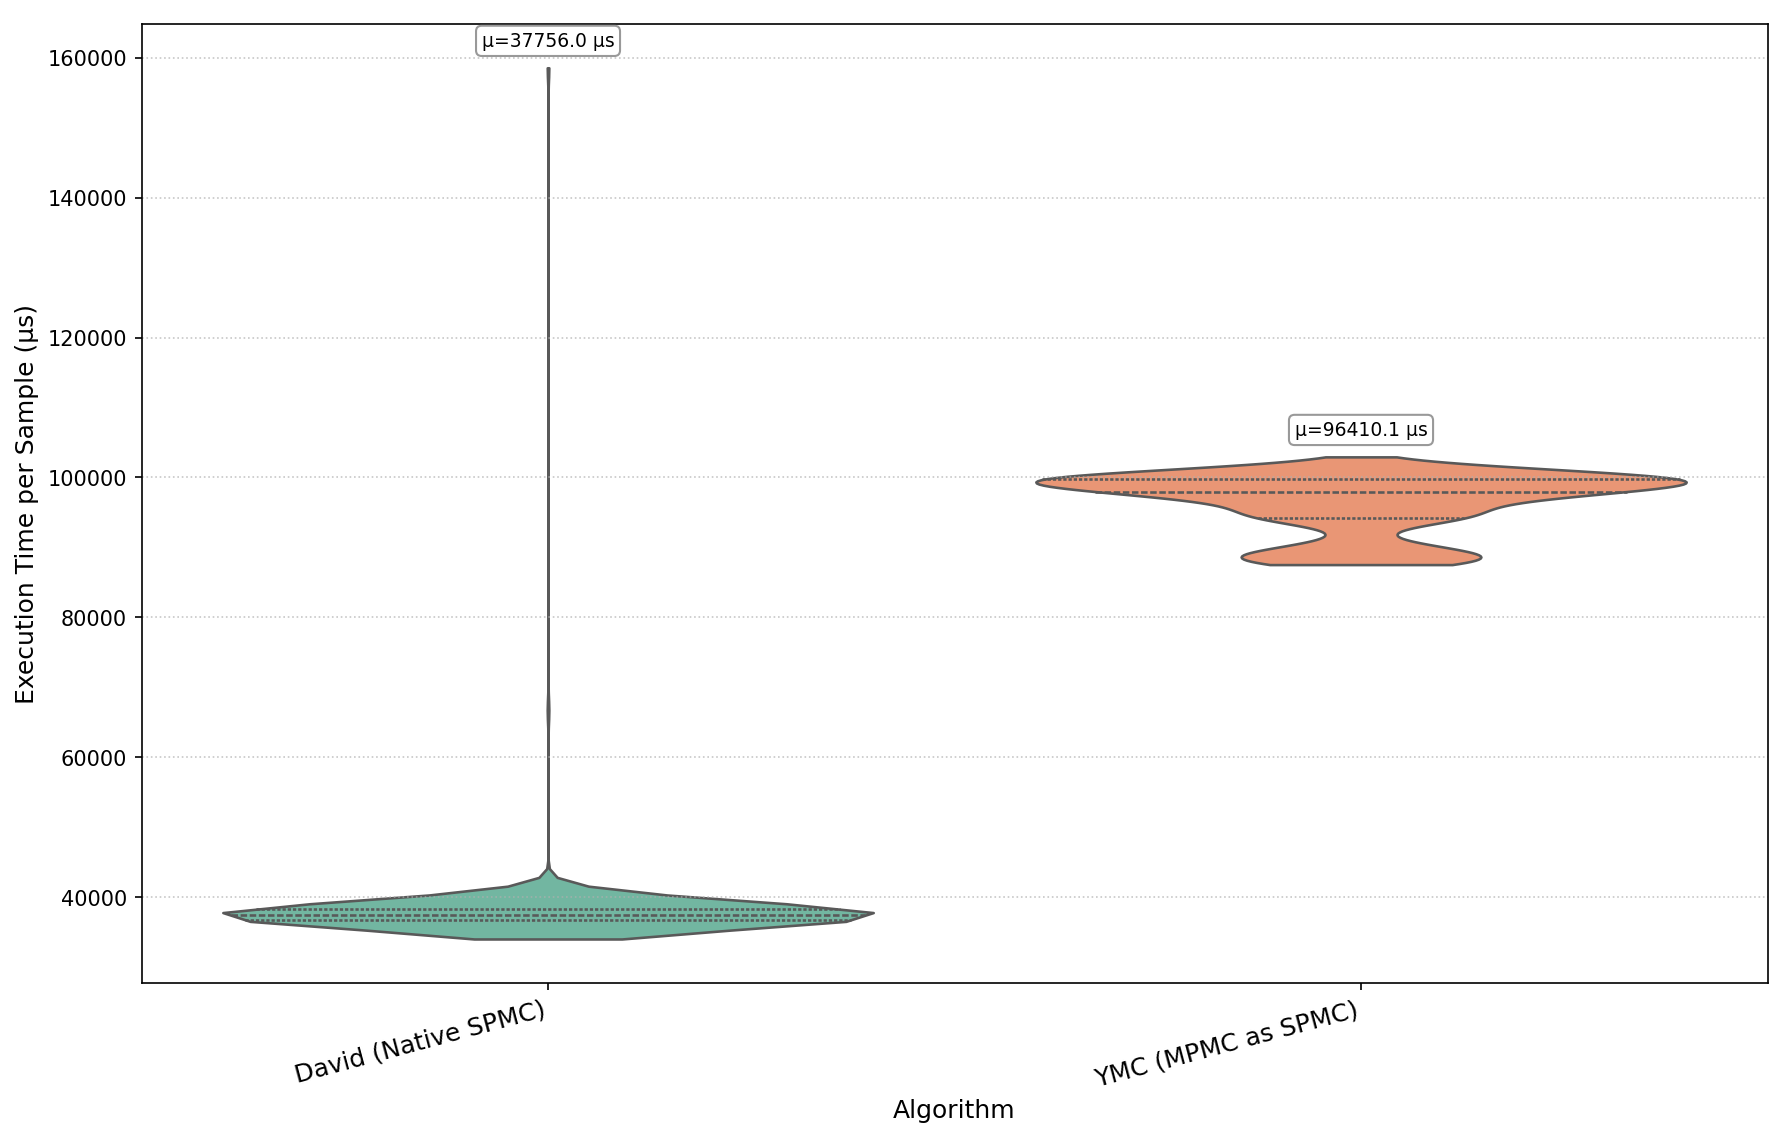
\includegraphics[width=\textwidth]{images/results/best_in_spmc_performance_violin_1P8C.png}
\end{figure}



\end{document}